\section{Data - Monte Carlo comparisons}
\label{sec:dataMCcomparisons}
% ---- ---- ---- ---- ---- ---- ---- ---- ---- ---- ---- ---- ---- ---- ---- ---- ---- ---- ---- ---- ---- ---- ----

To assess the quality of the modeling provided by the MC simulation we
make comparisons between the MC shape, normalized to the number of
collected events in data, for the background compared to the overall
data yield after applying the event selection criteria.  We show the
distributions of various kinematic variables after applying all the
selection cuts in Figures ~\ref{fig:mu_jet_pt}-\ref{fig:mu_mjj} for
the muon+jets sample and in Figures
~\ref{fig:elec_jet_pt}-\ref{fig:elec_mjj} for the electron+jets
sample.  Eventually, Figure~\ref{fig:lep_mlvjj} shows the four-body
invariant mass, for electrons (on the left) and muons (on the right).
The MC has been been corrected for lepton reconstruction efficiency
and the trigger efficiency.  Besides the kinematics of the single
objects, we show here also the variables that are used in the MVA
discriminant that maximizes the signal-over-background ratio.  Seeing
reasonable agreement gives us confidence in the qualitative aspects of
the MC modeling.
%%%%%%%%%%%%%%%%%%%%%%%%%%%%
\begin{figure}[ht]
  {\centering
    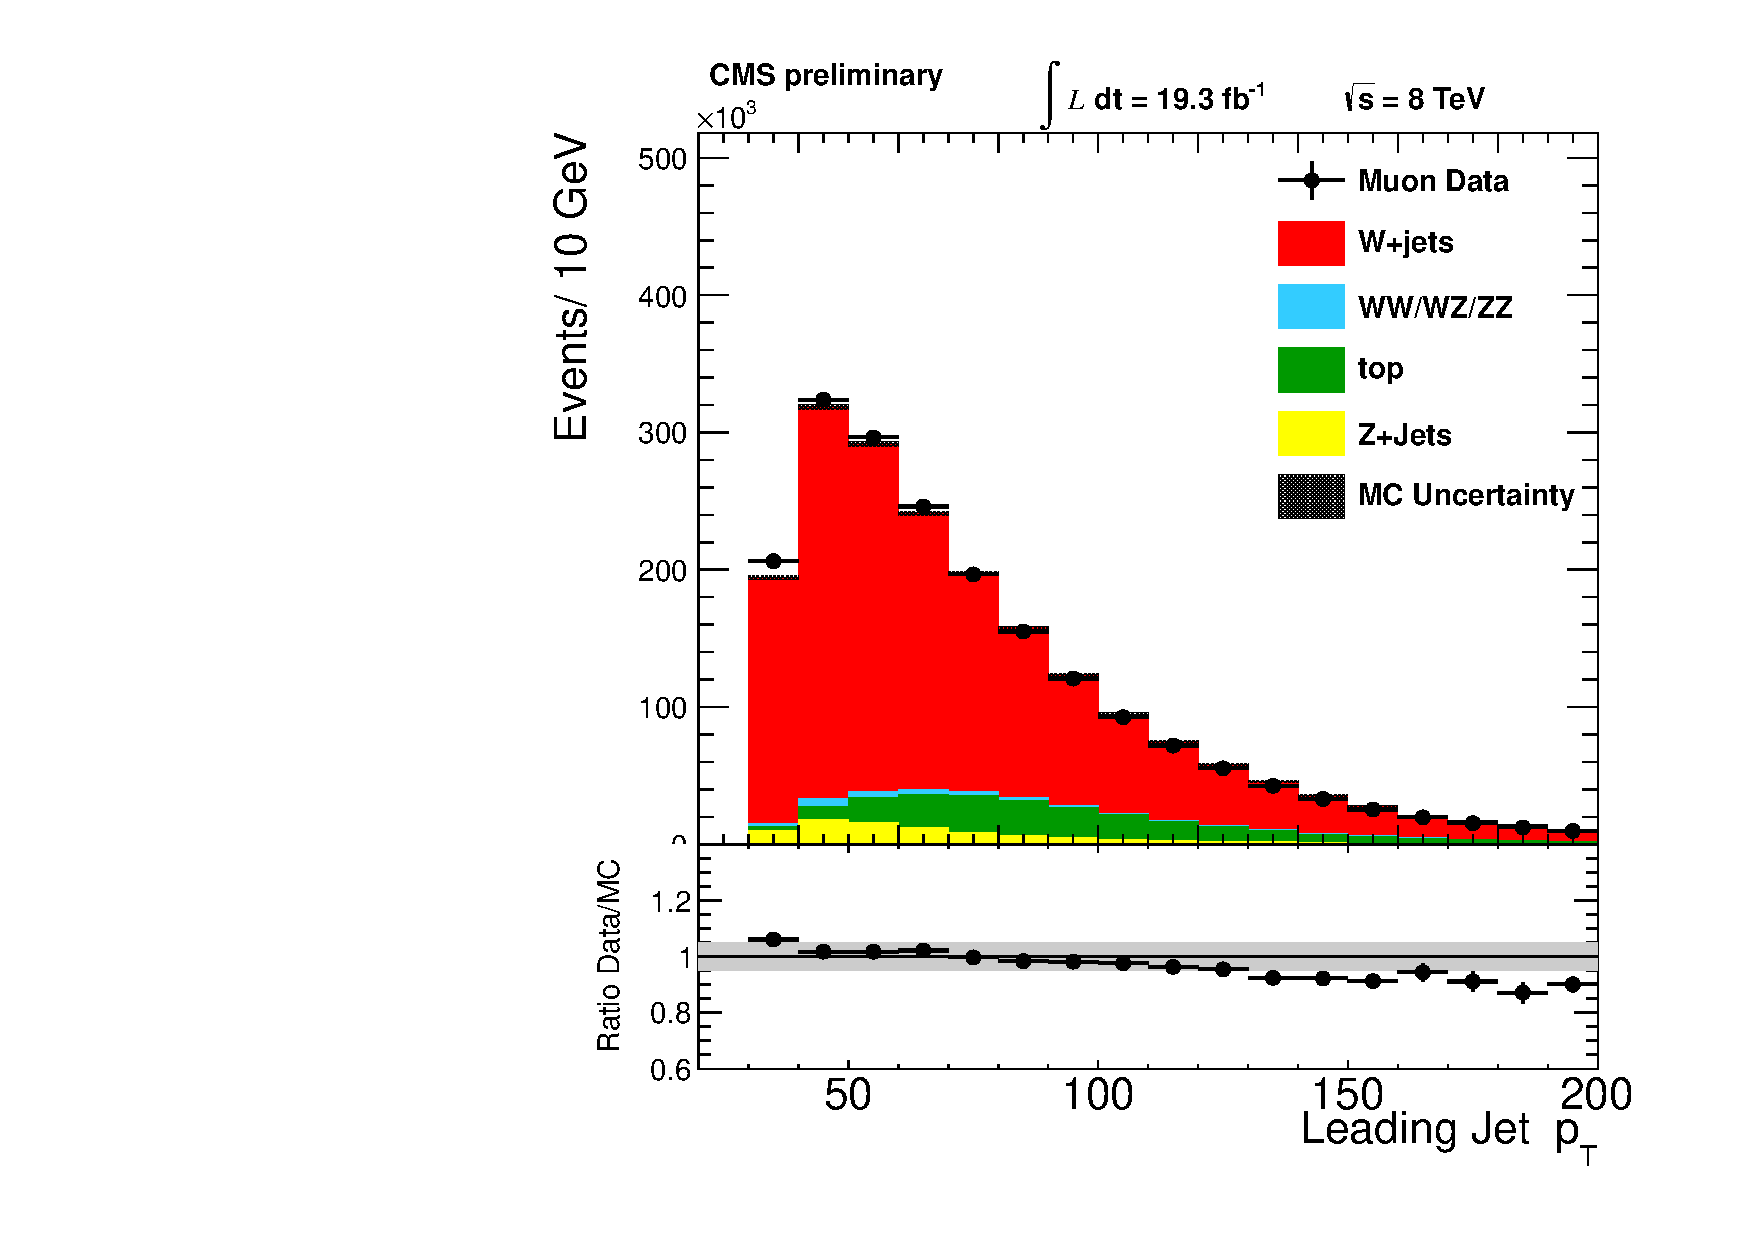
\includegraphics[width=0.49\textwidth]{plots/2012_DataMC/mu_jetld_pt.pdf}
    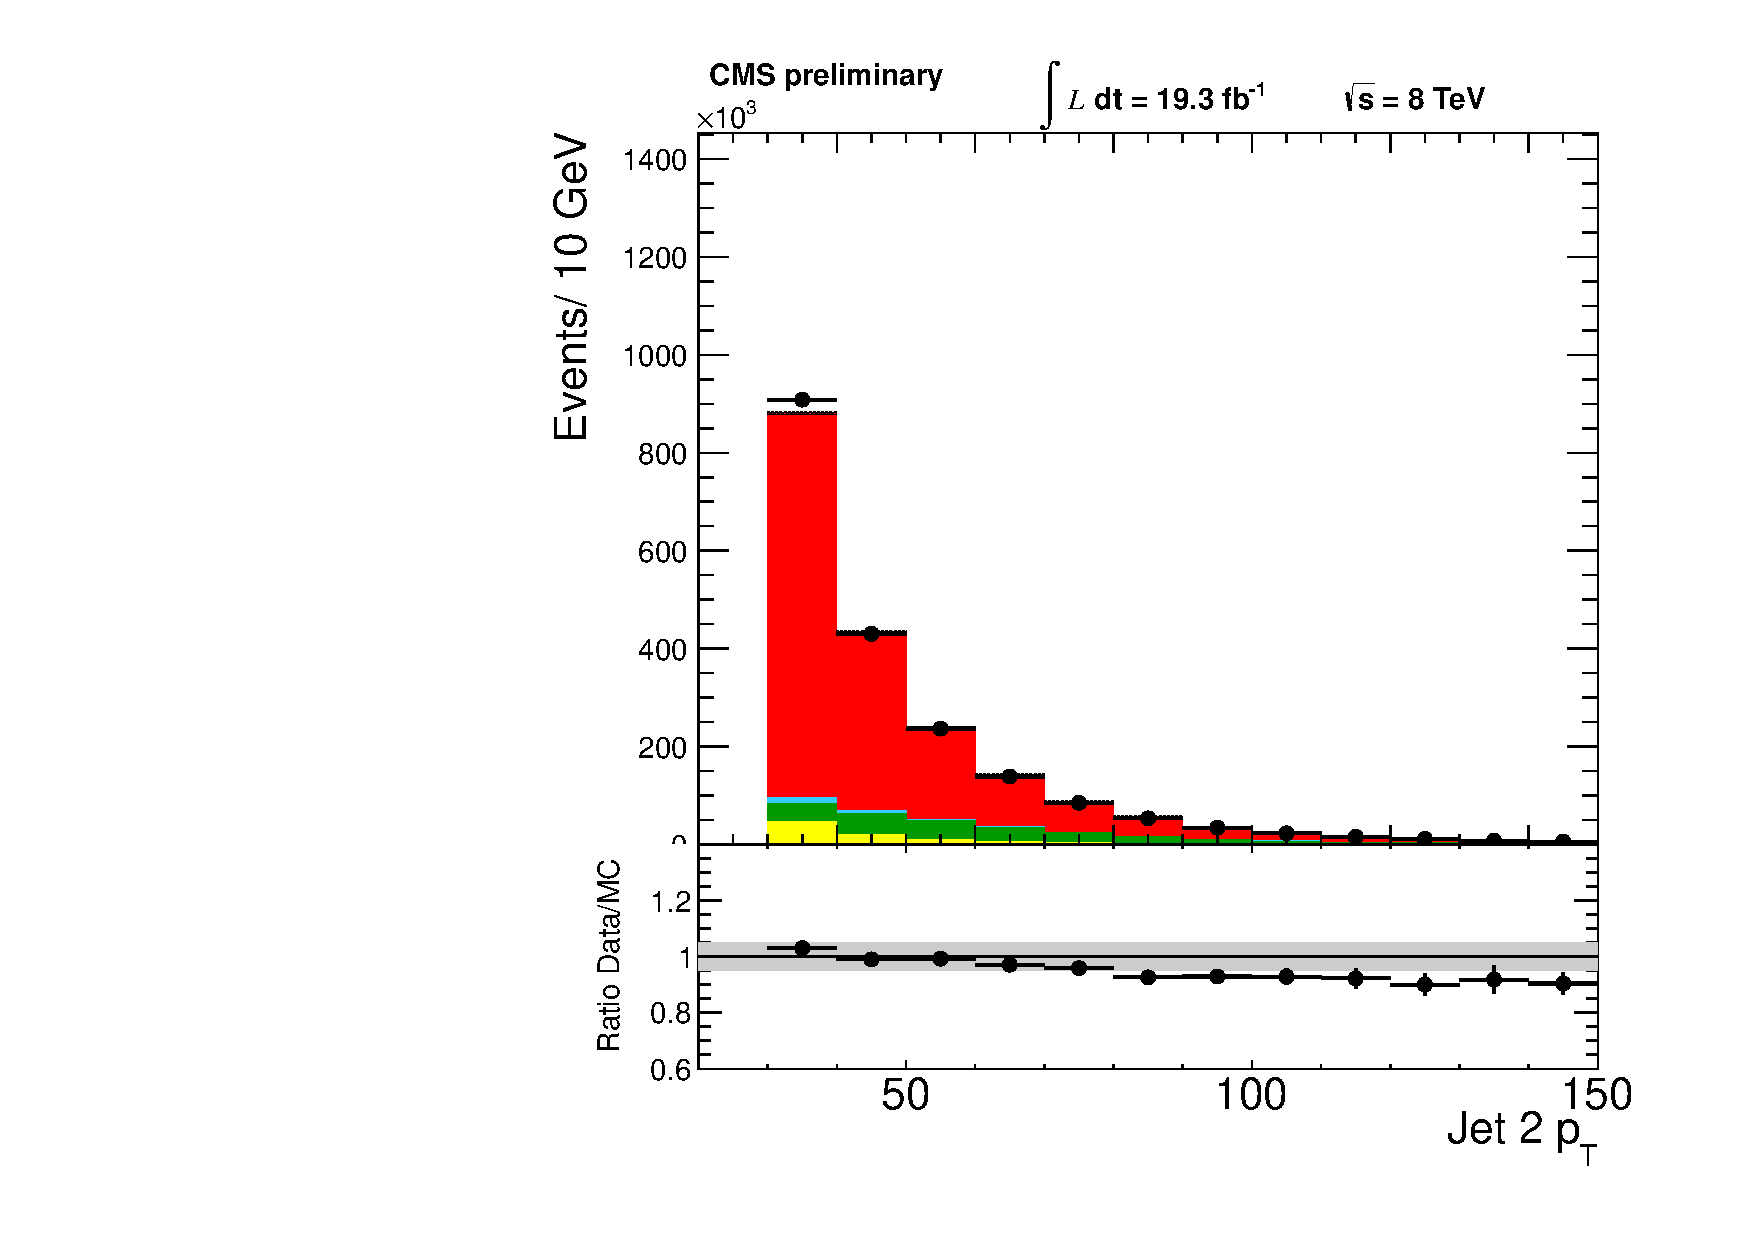
\includegraphics[width=0.49\textwidth]{plots/2012_DataMC/mu_jetnt_pt.pdf}
    \caption{Comparison of the leading jet (left) and 
      the second jet (right) $p_{T}$ distributions from data and MC for the muon+jets
      selection.}
    \label{fig:mu_jet_pt}}
\end{figure}
%%%%%%%%%%%%%%%%%%%%%%%%%%%%
\begin{figure}[h!t]
  {\centering
    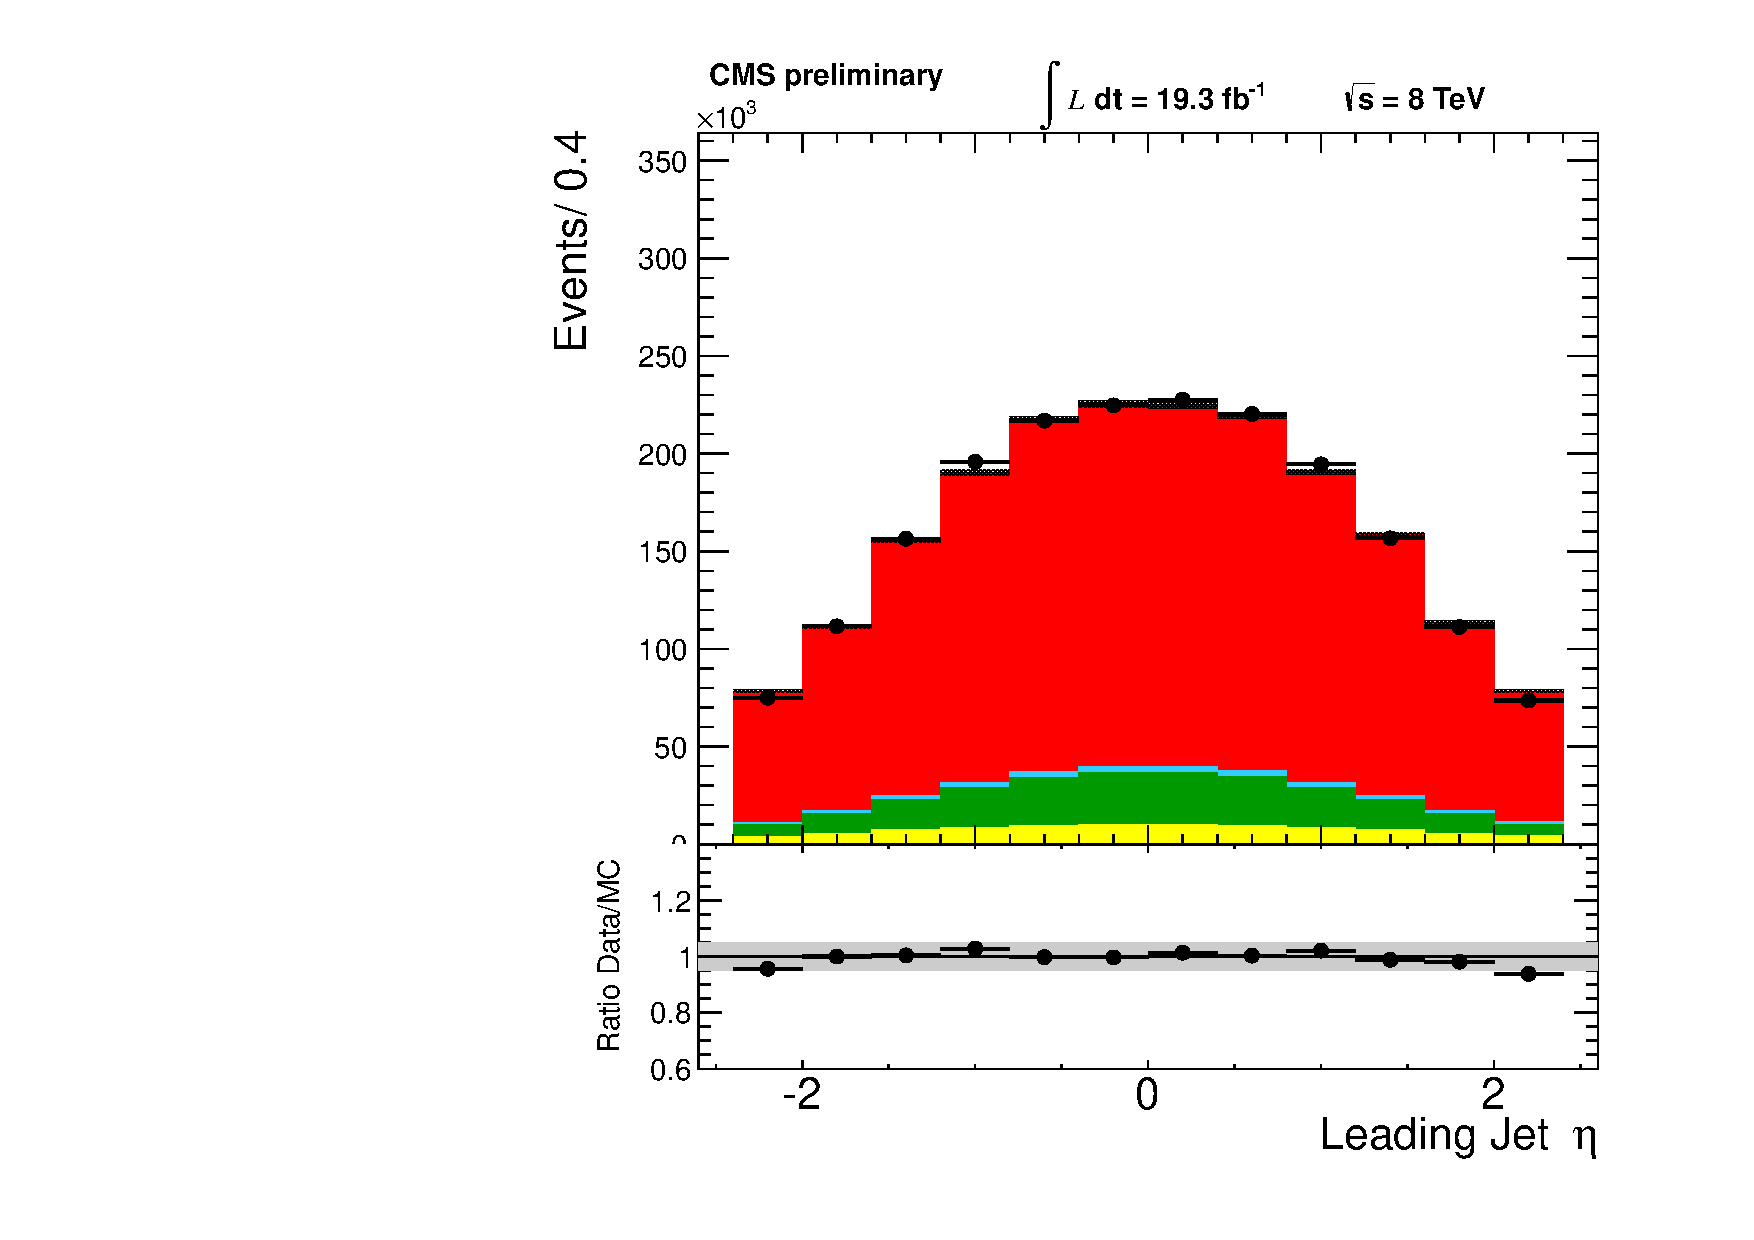
\includegraphics[width=0.49\textwidth]{plots/2012_DataMC/mu_jetld_eta.pdf}
    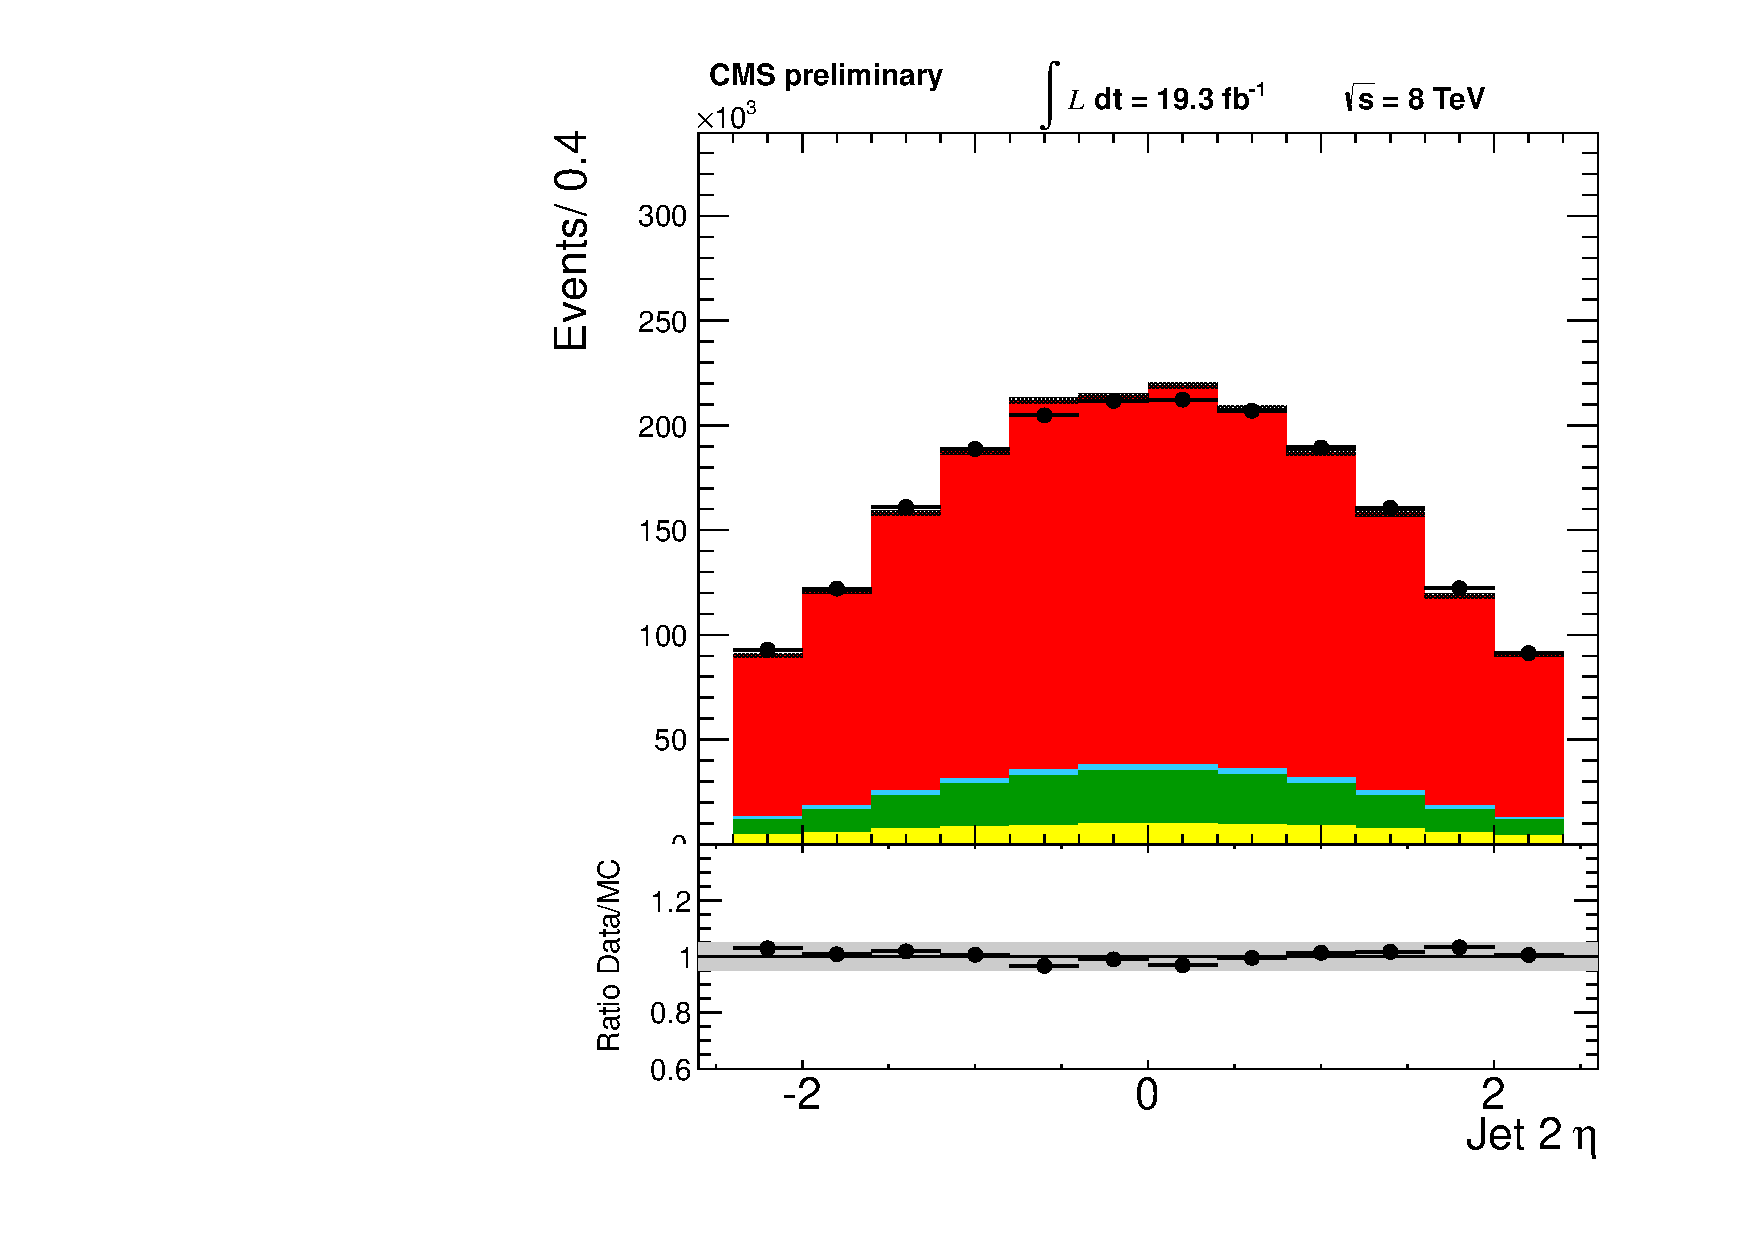
\includegraphics[width=0.49\textwidth]{plots/2012_DataMC/mu_jetnt_eta.pdf}
    \caption{Comparison of the leading jet $\eta $ (left) and the
    second leading jet $\eta $ (right) distributions from data and MC
    for the muon+jets selection.  }
\label{fig:mu_jet_eta}}
\end{figure}
%%%%%%%%%%%%%%%%%%%%%%%%%%%%
\begin{figure}[h!t]
  {\centering
    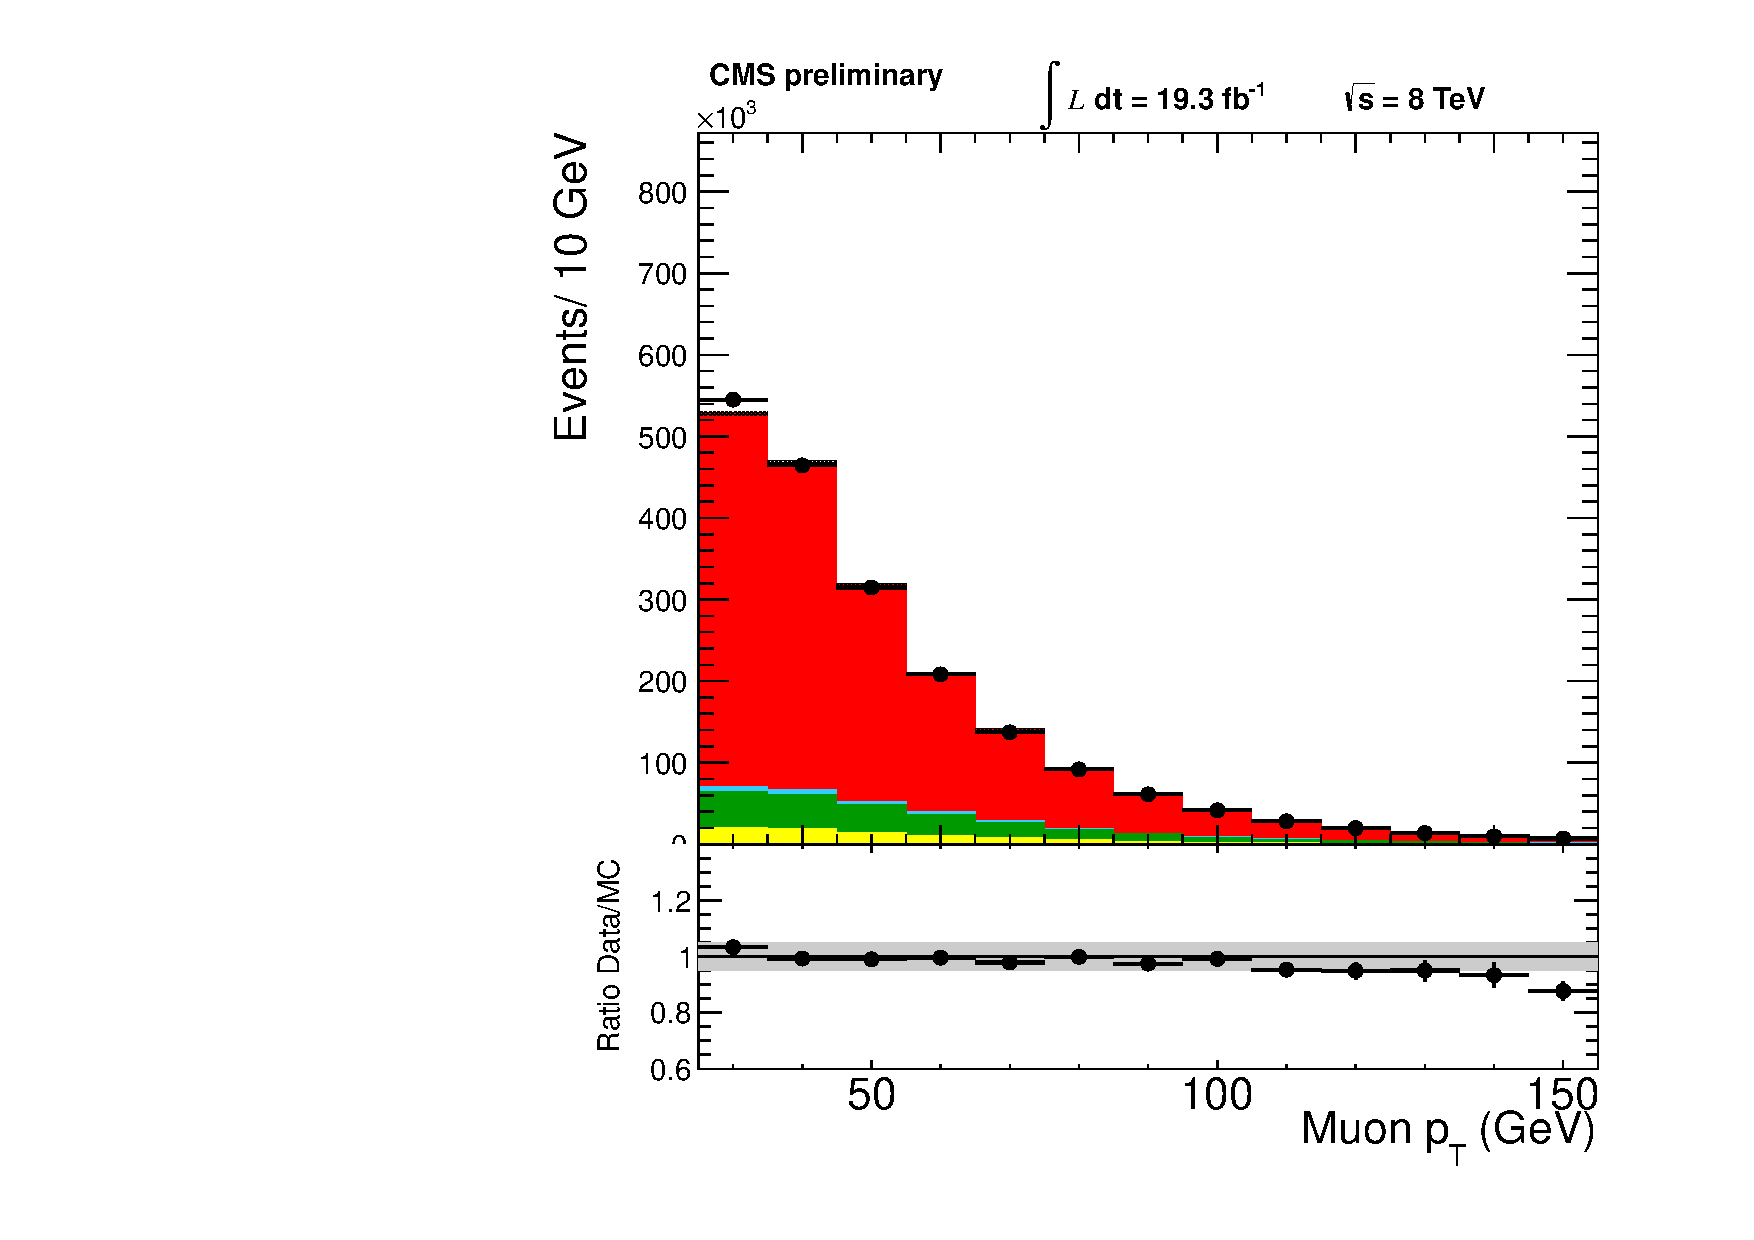
\includegraphics[width=0.49\textwidth]{plots/2012_DataMC/mu_W_muon_pt.pdf}
    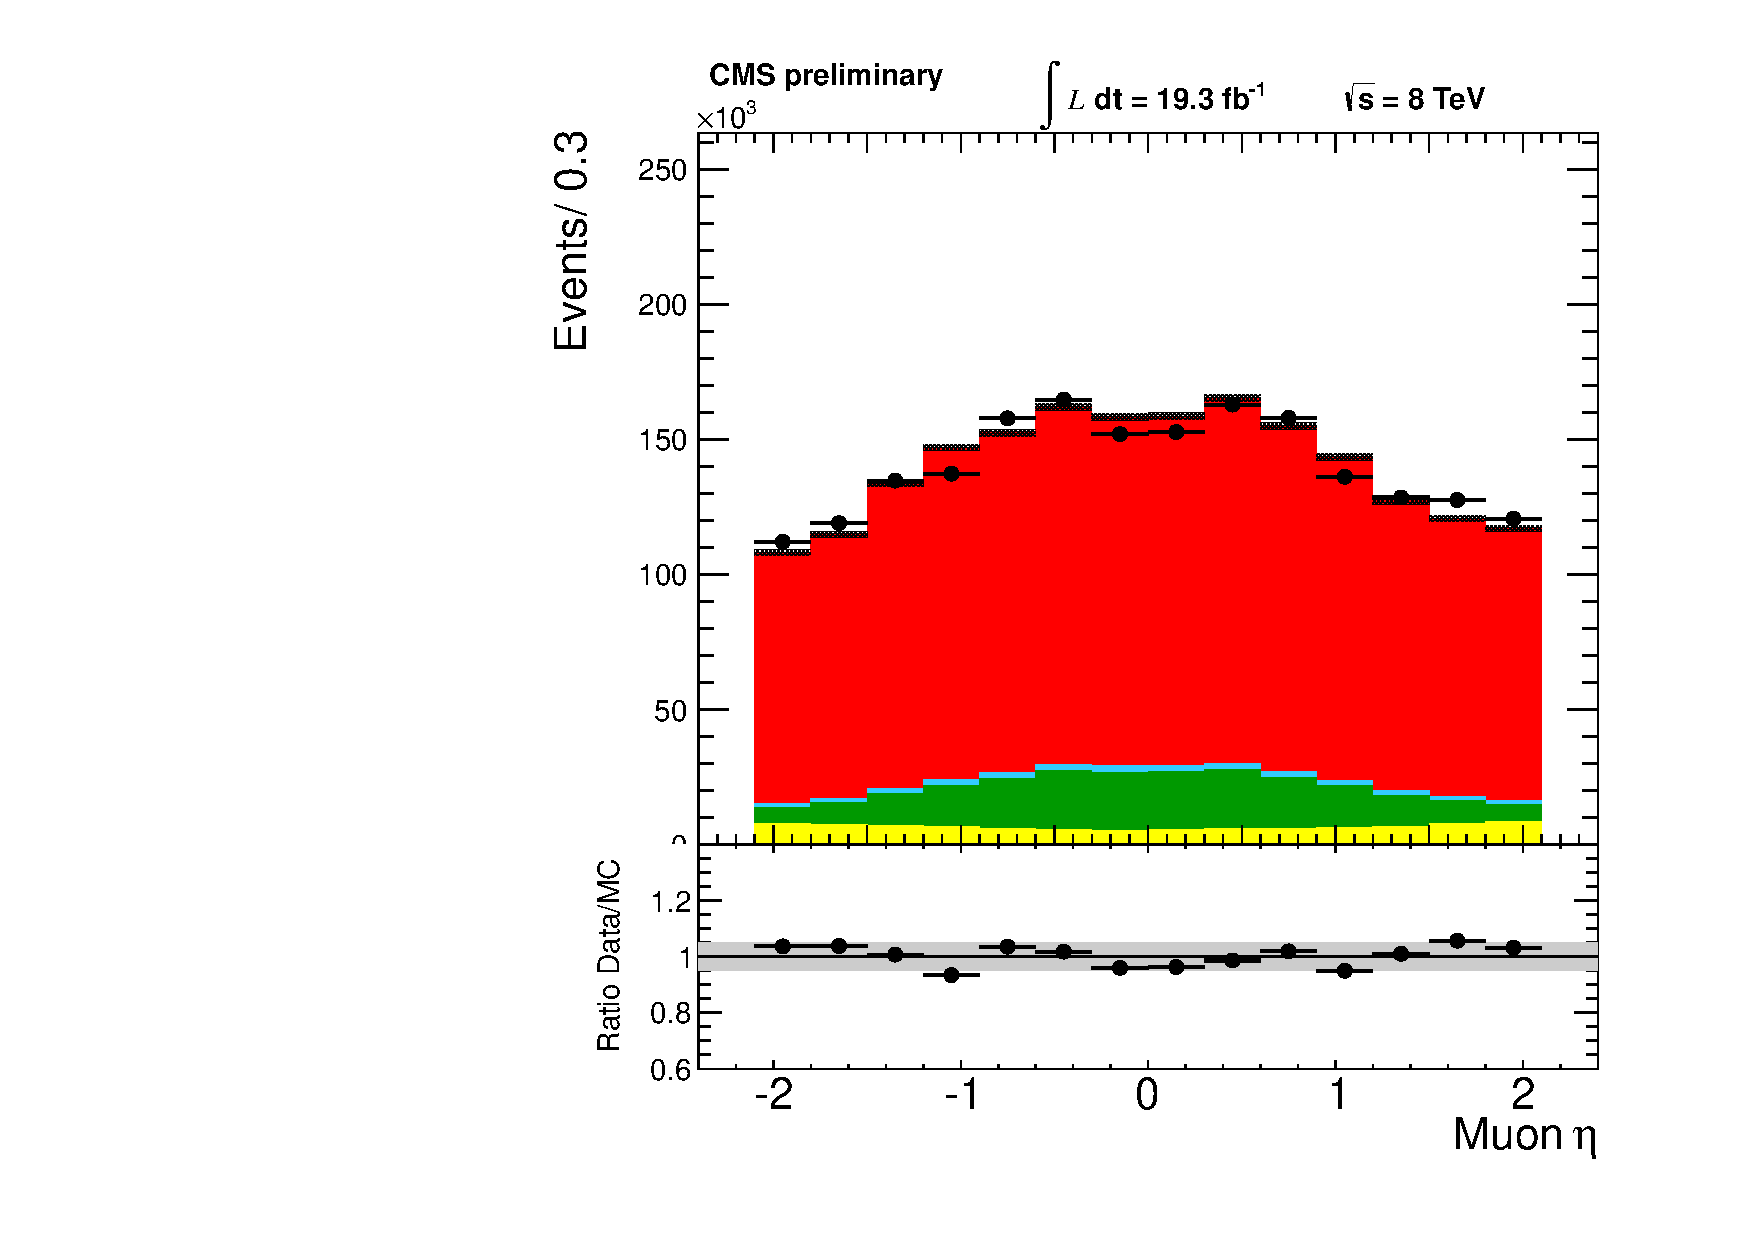
\includegraphics[width=0.49\textwidth]{plots/2012_DataMC/mu_W_muon_eta.pdf}
    \caption{Comparison of the muon $p_{T} $ (left) and the
    muon $\eta $ (right) distributions from data and MC for the
    muon+jets selection. 
    }
   \label{fig:mu_muon}}
\end{figure}

%%%%%%%%%%%%%%%%%%%%%%%%%%%%
\begin{figure}[h!t]
  {\centering
    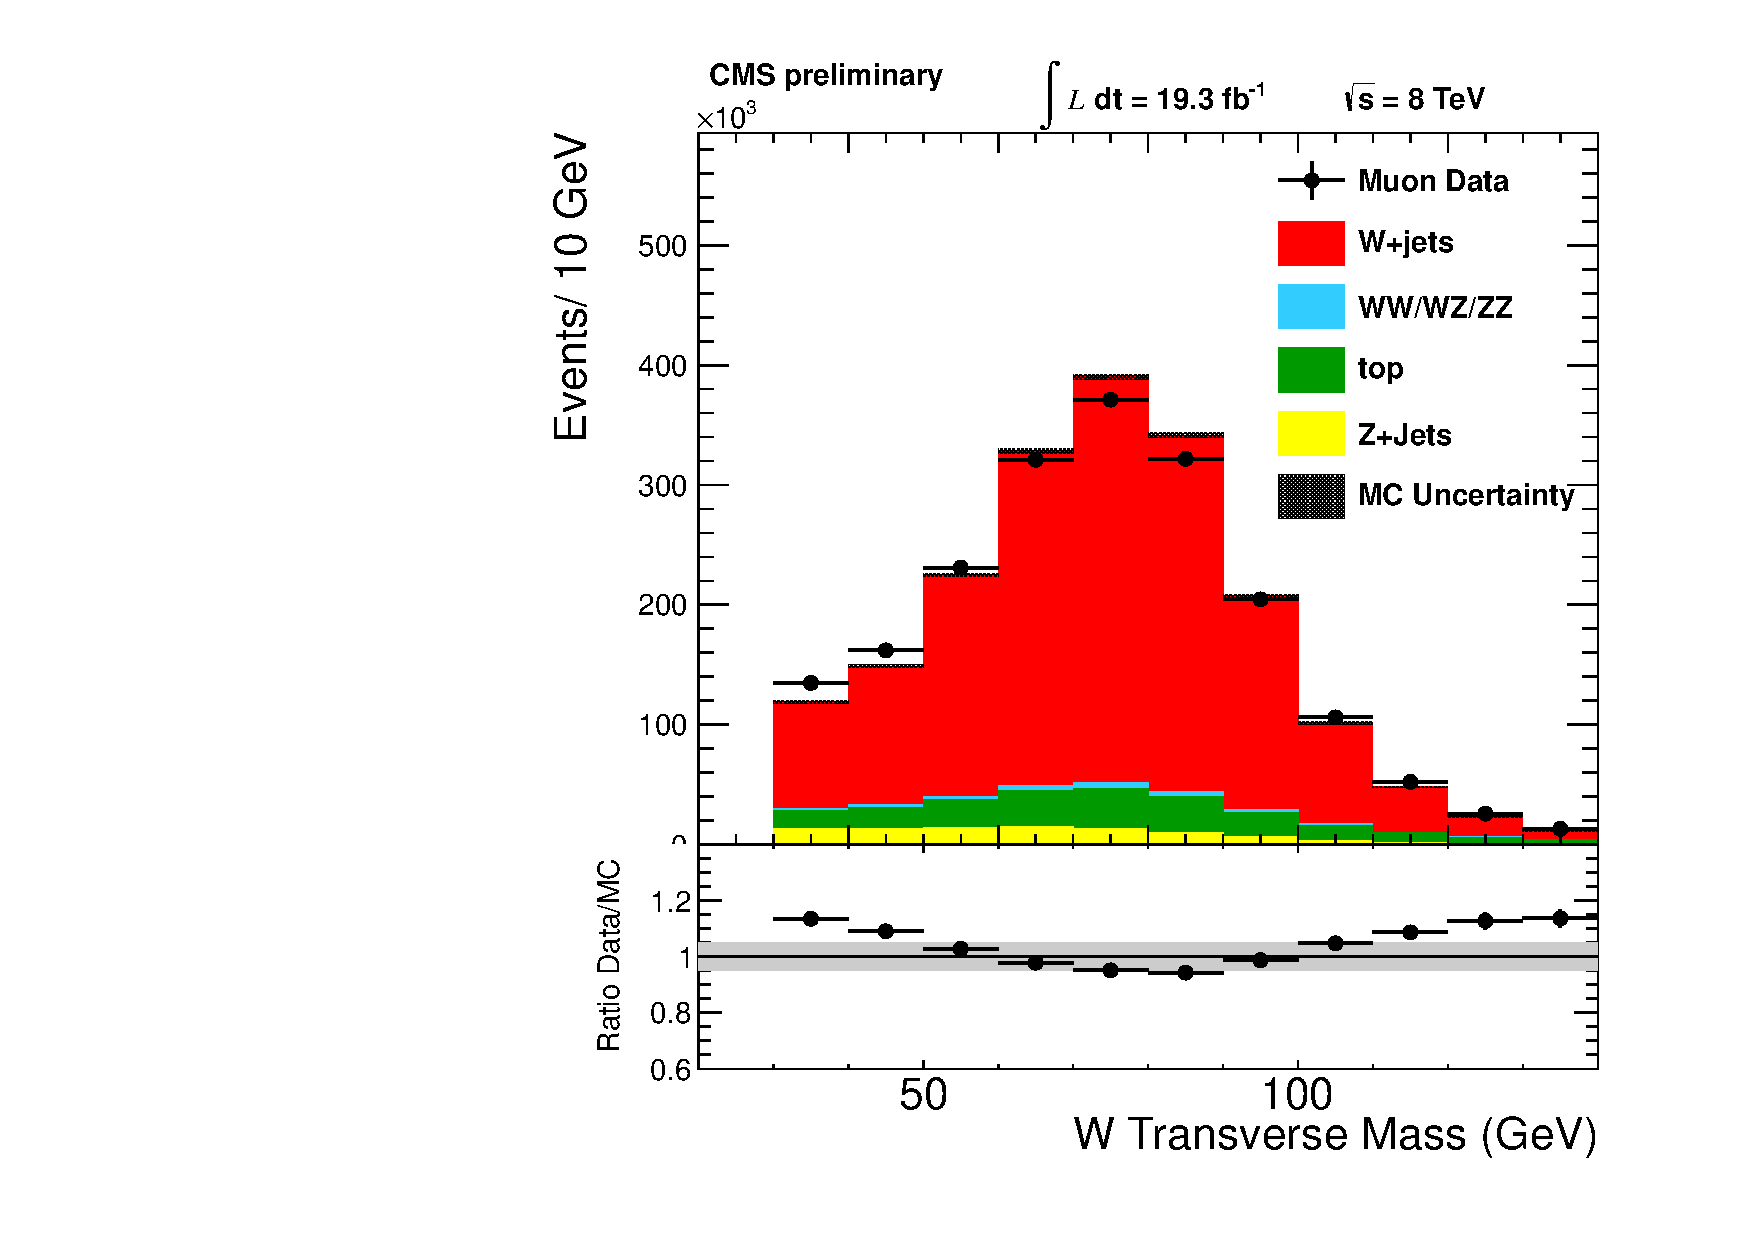
\includegraphics[width=0.49\textwidth]{plots/2012_DataMC/mu_W_mt.pdf}
    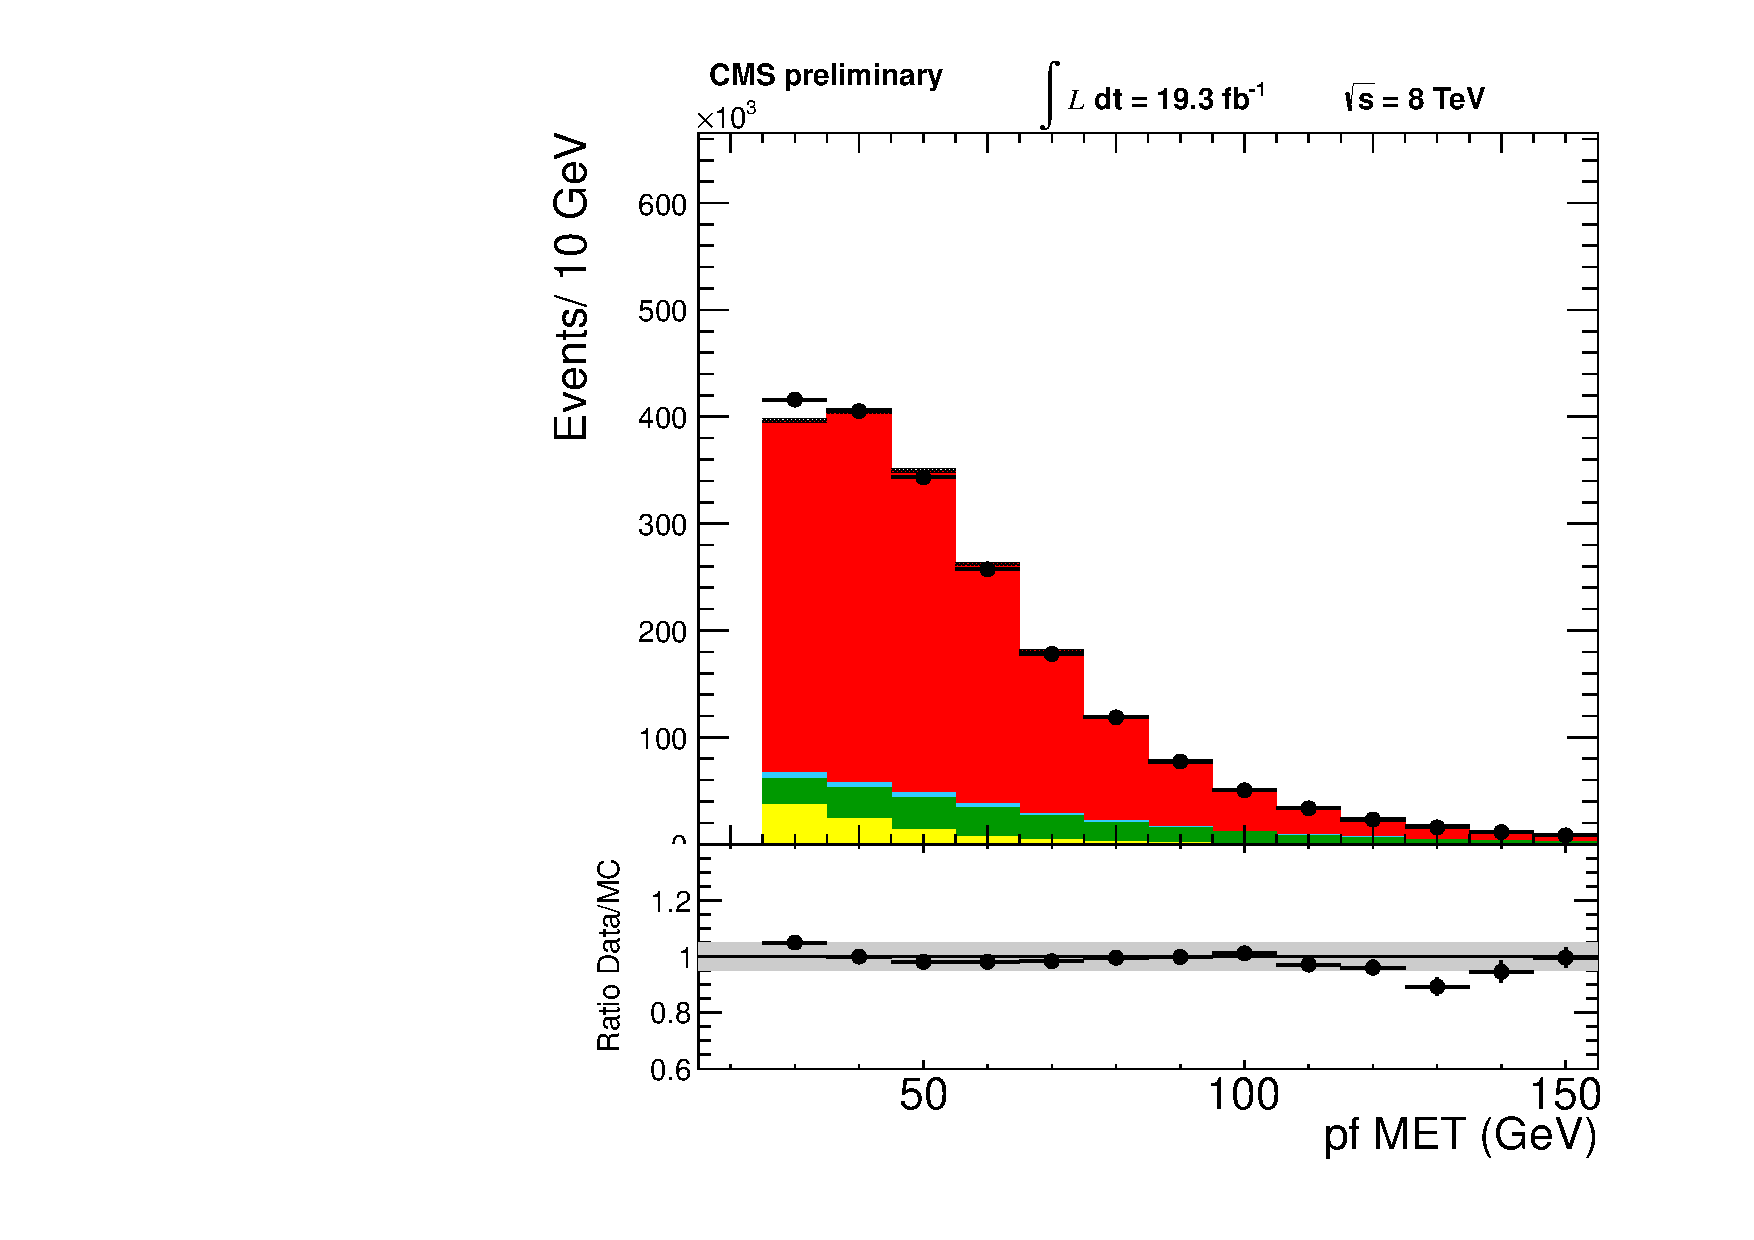
\includegraphics[width=0.49\textwidth]{plots/2012_DataMC/mu_event_met_pfmet.pdf}
    \caption{Comparison of the distributions from data and MC of the
     transverse mass of the muon / MET system (left) and the MET (right)
    for the muon+jets selection.
    }
    \label{fig:mu_W_Mt}}
\end{figure}
%%%%%%%%%%%%%%%%%%%%%%%%%%%%
\begin{figure}[h!t]
  {\centering
    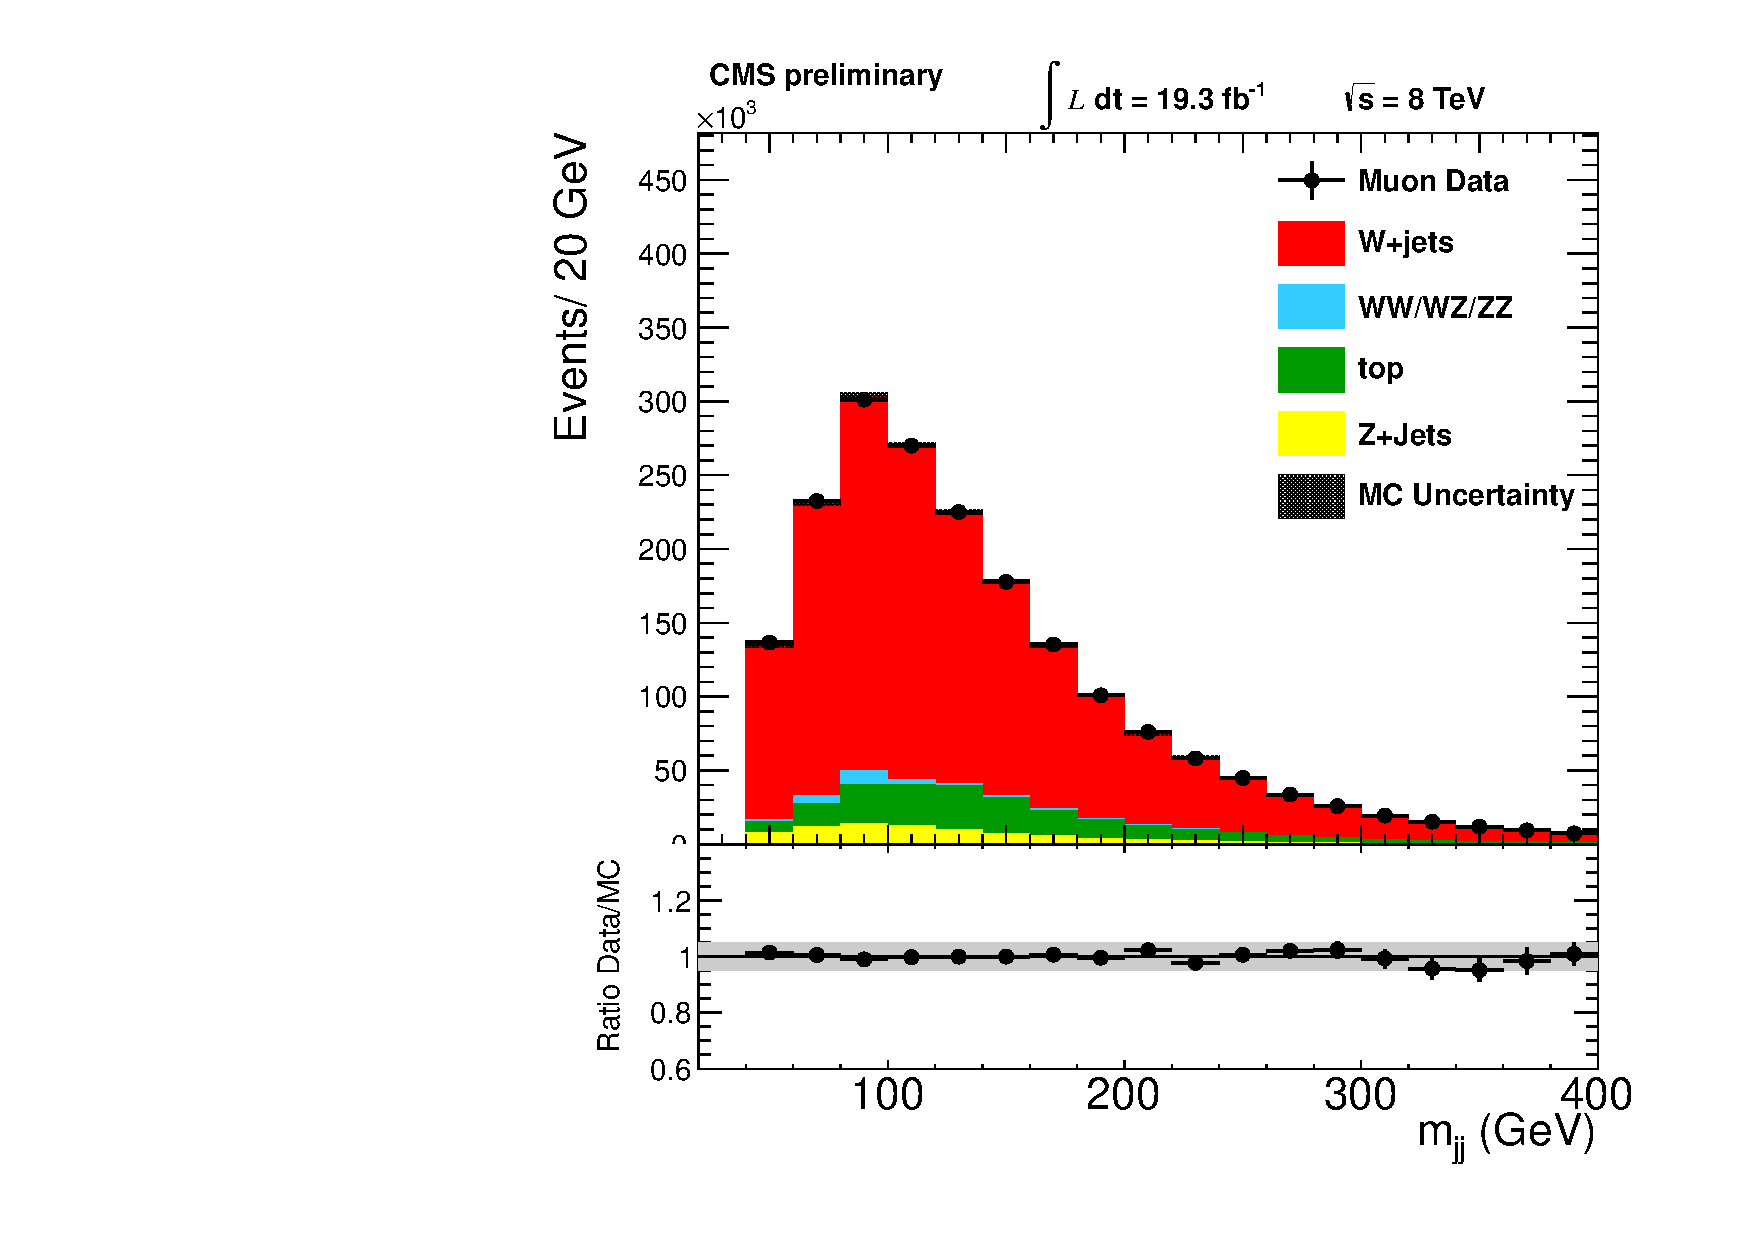
\includegraphics[width=0.49\textwidth]{plots/2012_DataMC/mu_mjj.pdf}
    \caption{Comparison of the dijet mass ($m_{JJ}$) distributions from data and MC for 
      the muon+jets selection. }
    \label{fig:mu_mjj}}
\end{figure}

%%%%%%%%%%%%%%%%%%%%%%%%%%%%
%%%%%%%%%%%%%%%%%%%%%%%%%%%%
\begin{figure}[h!t]
  {\centering
    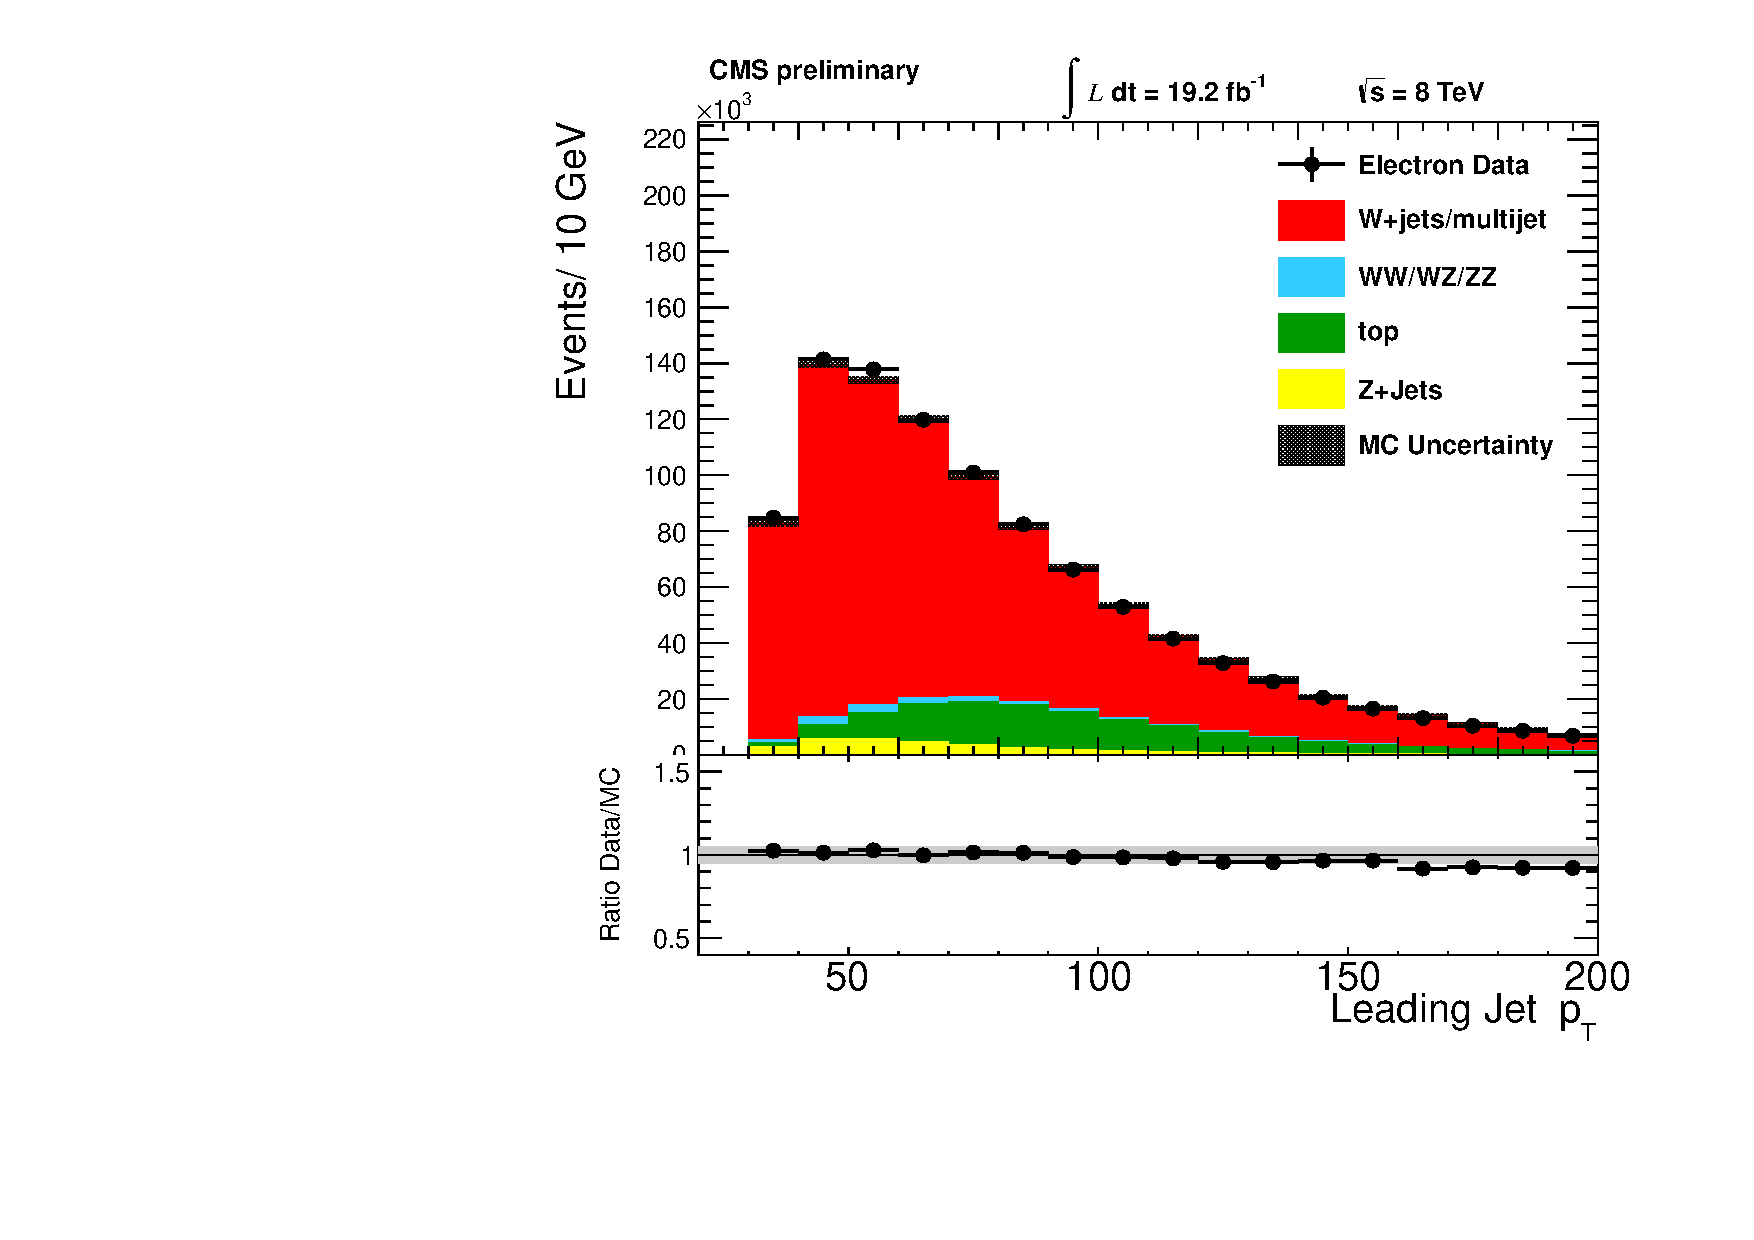
\includegraphics[width=0.49\textwidth]{plots/2012_DataMC/el_jetld_pt.pdf}
    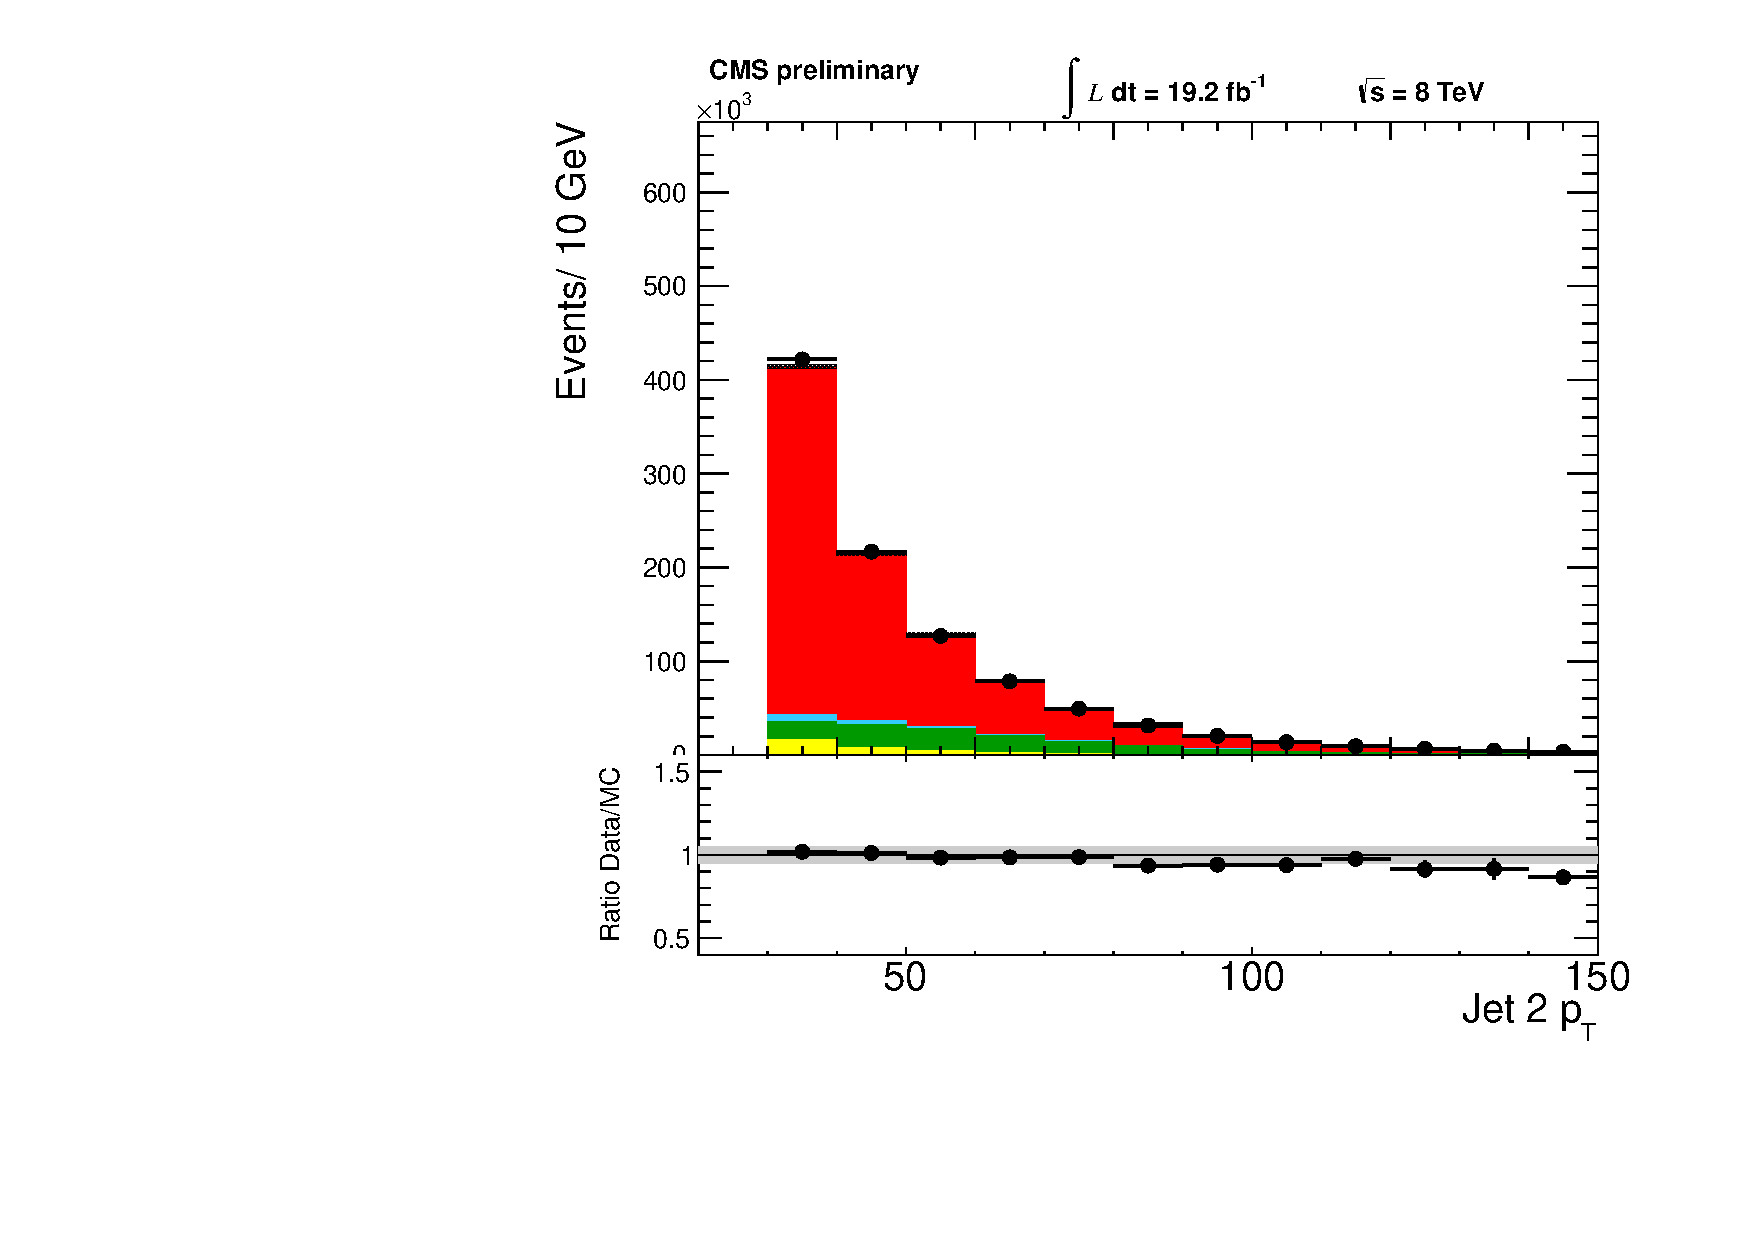
\includegraphics[width=0.49\textwidth]{plots/2012_DataMC/el_jetnt_pt.pdf}
    \caption{Comparison of the leading jet $p_{T} $ (left) and the
      second leading jet $p_{T} $ (right) distributions from data and MC
      for the electron+jets selection.}
    \label{fig:elec_jet_pt}}
\end{figure}
%%%%%%%%%%%%%%%%%%%%%%%%%%%%
\begin{figure}[h!t]
  {\centering
    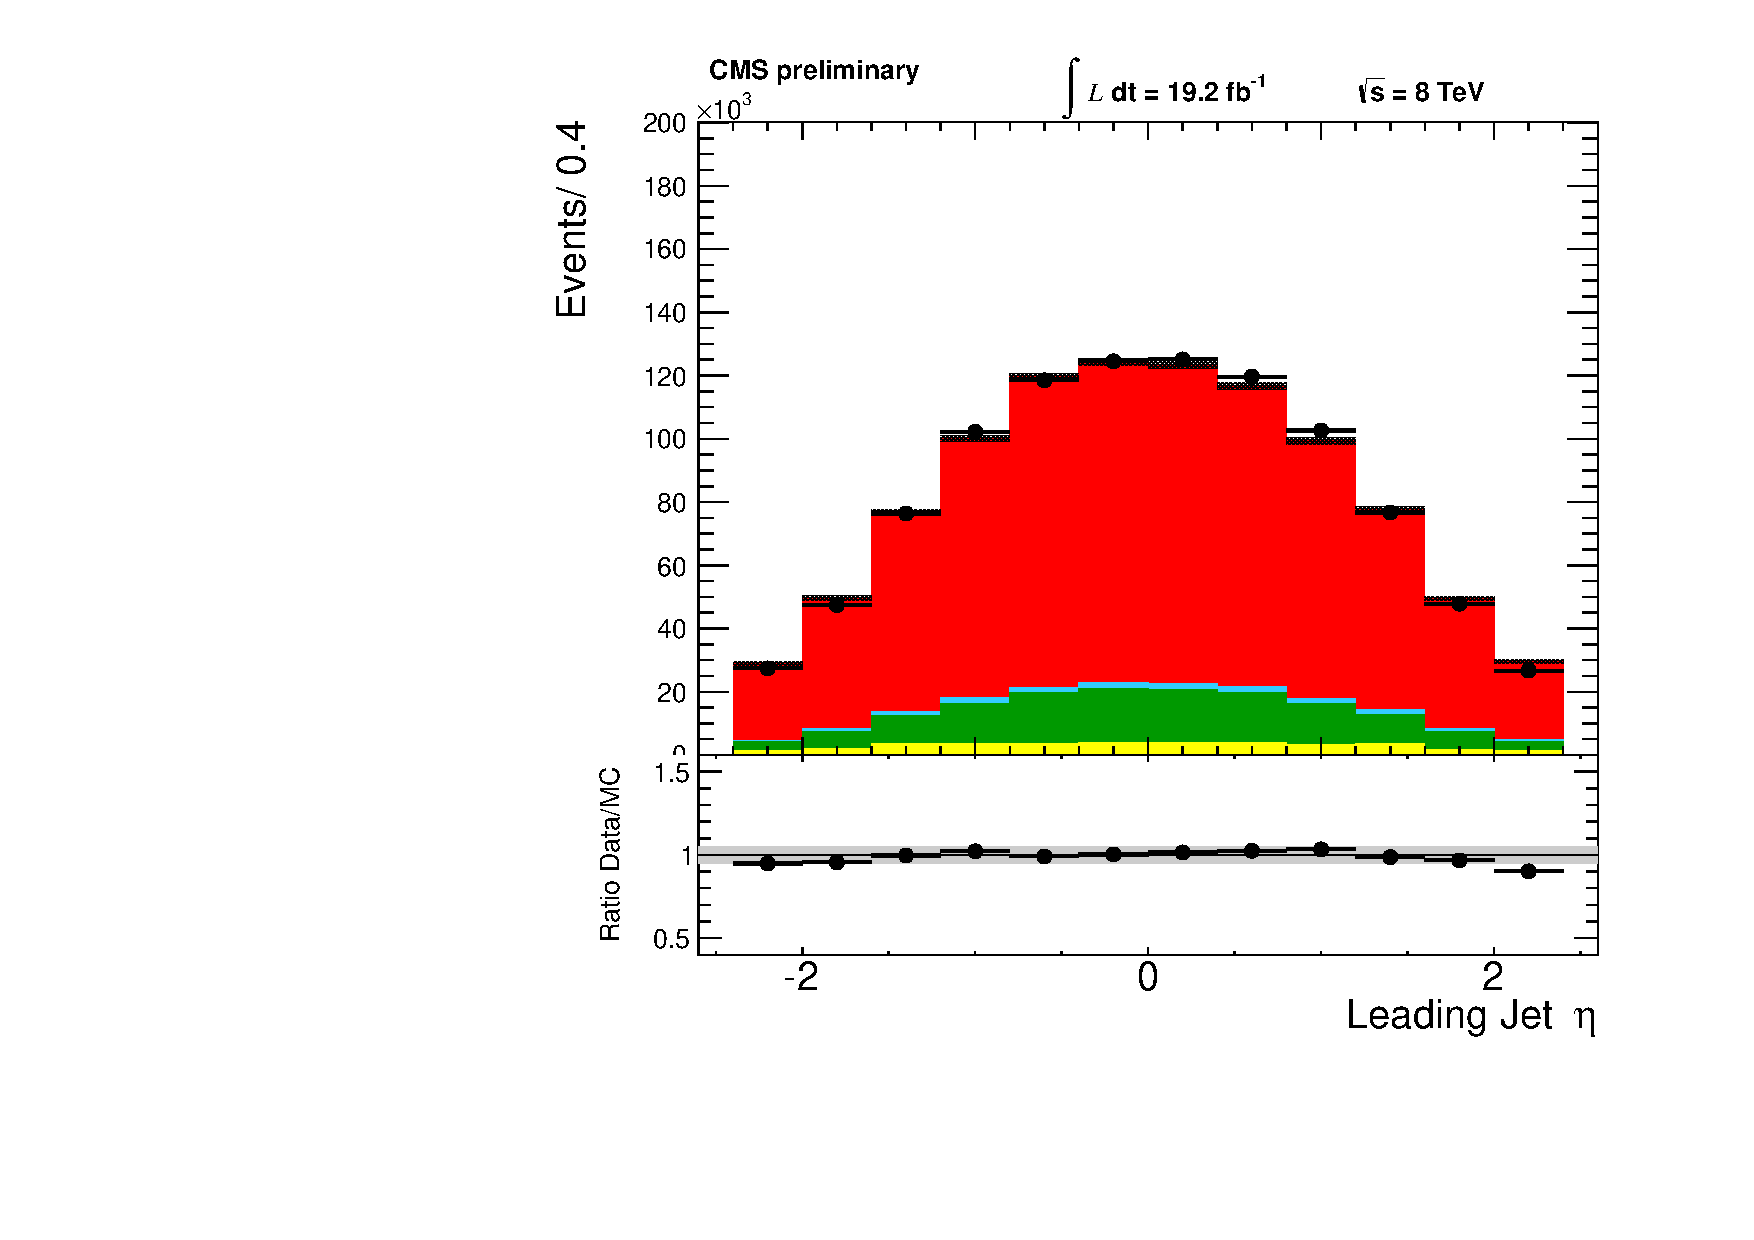
\includegraphics[width=0.49\textwidth]{plots/2012_DataMC/el_jetld_eta.pdf}
    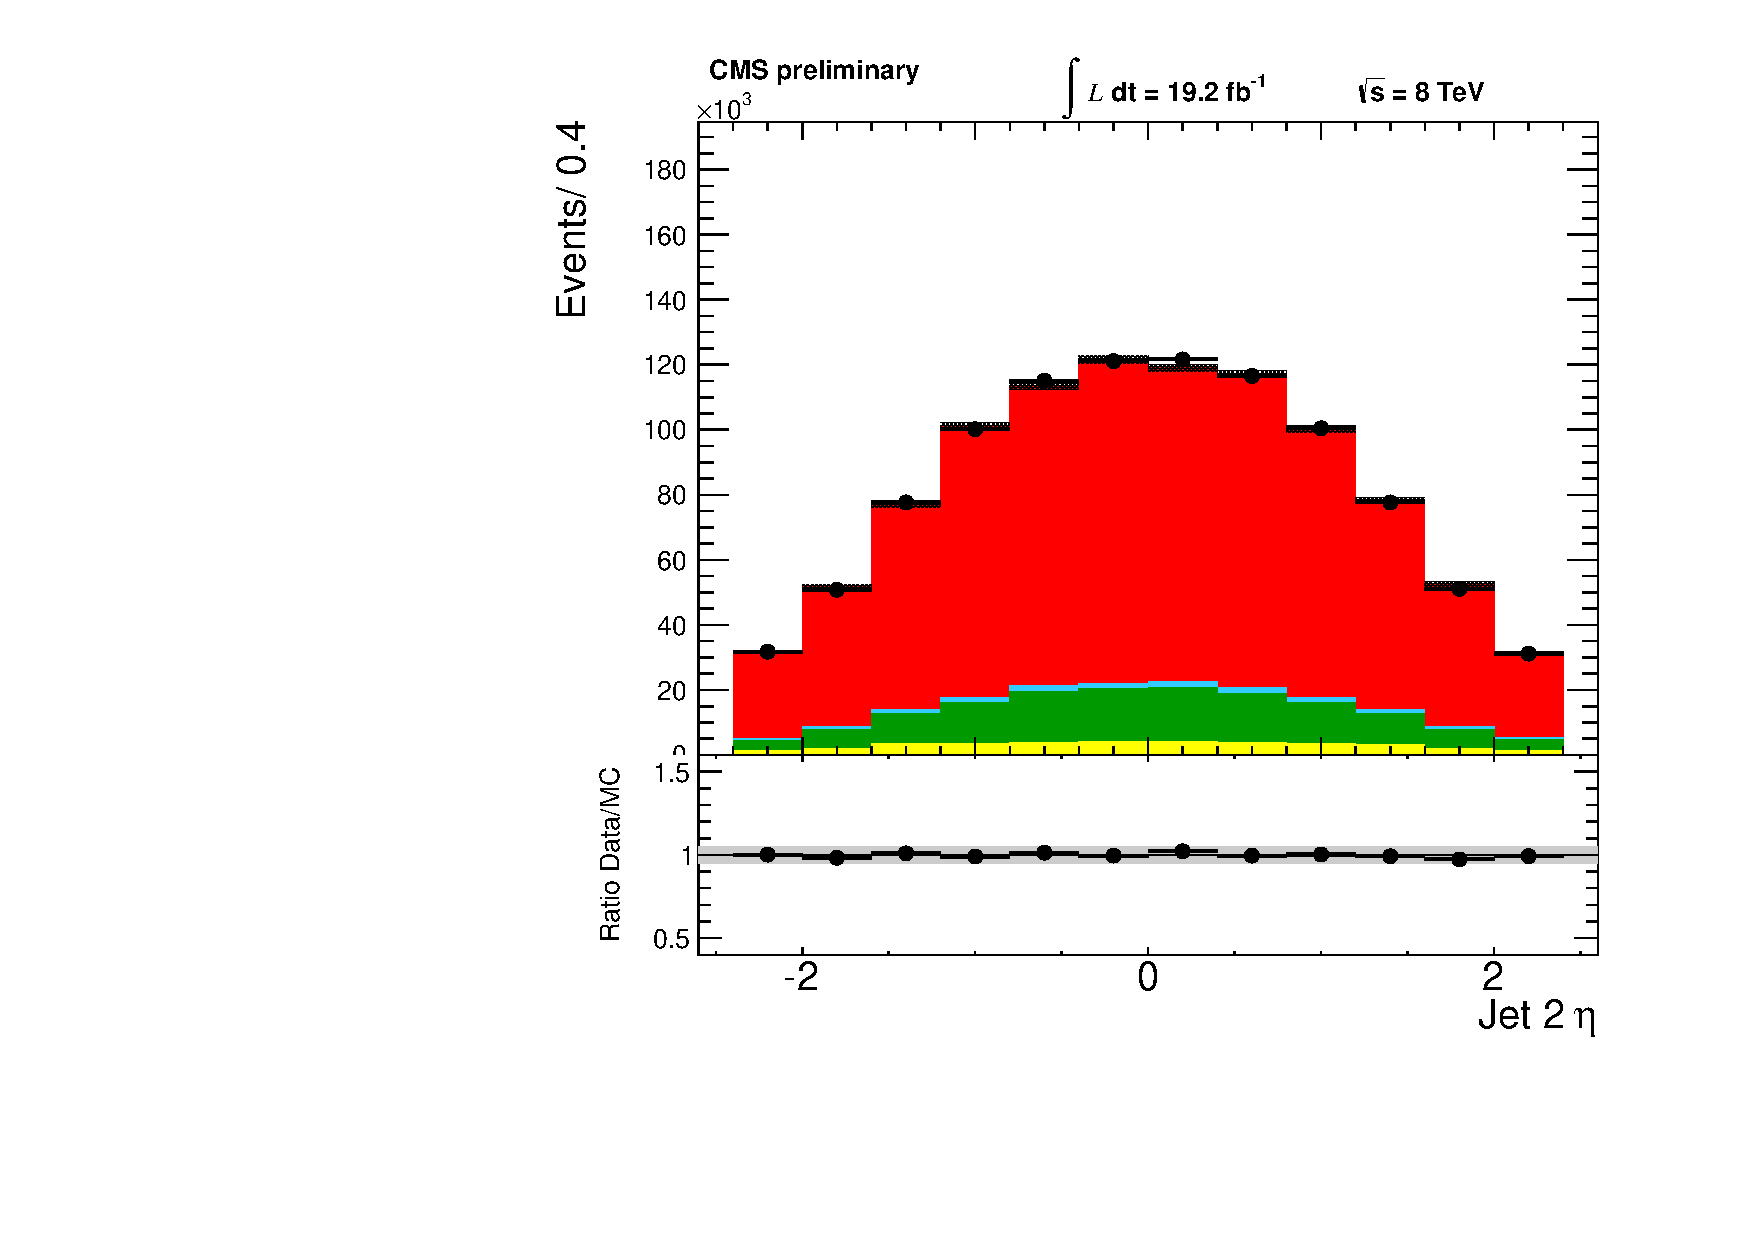
\includegraphics[width=0.49\textwidth]{plots/2012_DataMC/el_jetnt_eta.pdf}
    \caption{Comparison of the leading jet $\eta $ (left) and the
      second leading jet $\eta $ (right) distributions from data and MC for the electron+jets selection.}
    \label{fig:elec_jet_eta}}
\end{figure}
%%%%%%%%%%%%%%%%%%%%%%%%%%%%
\begin{figure}[h!t]
  {\centering
    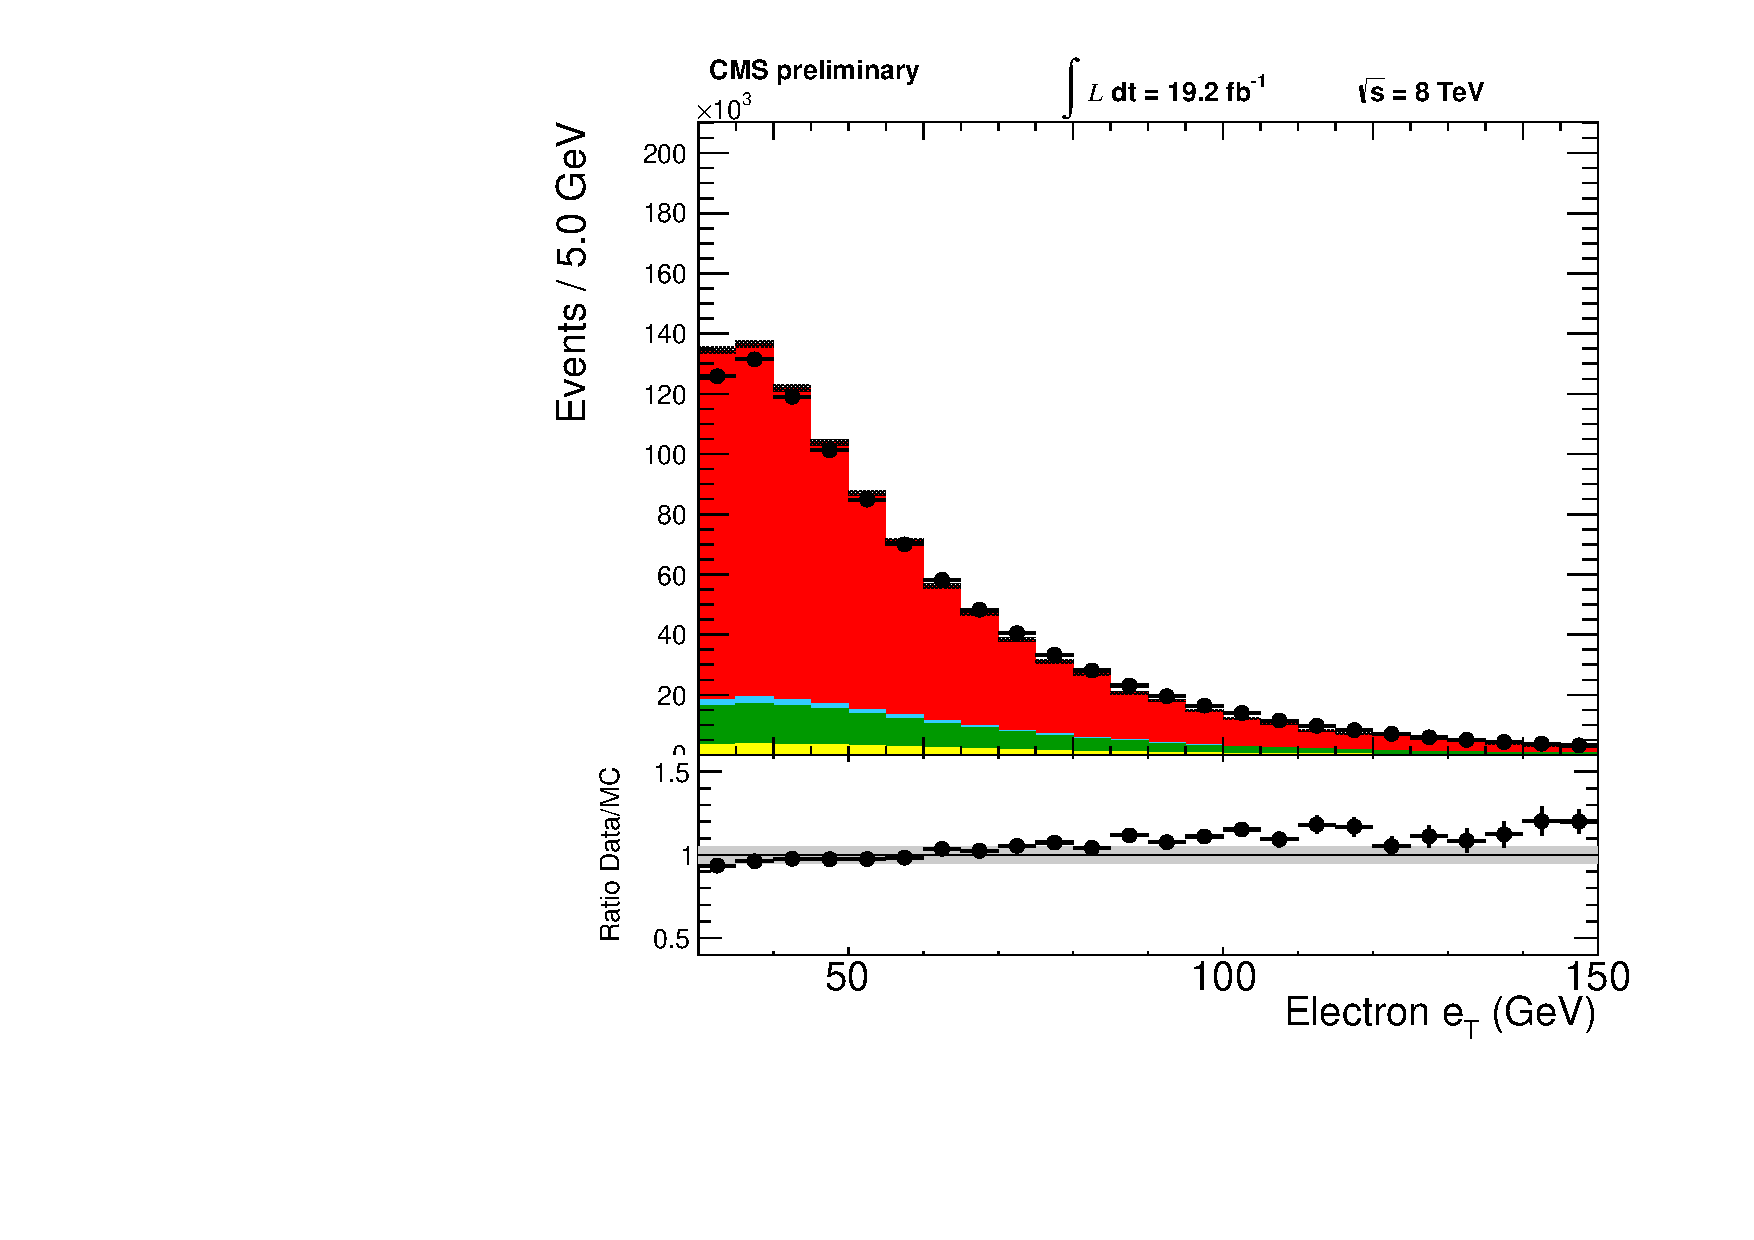
\includegraphics[width=0.49\textwidth]{plots/2012_DataMC/el_W_electron_et.pdf}
    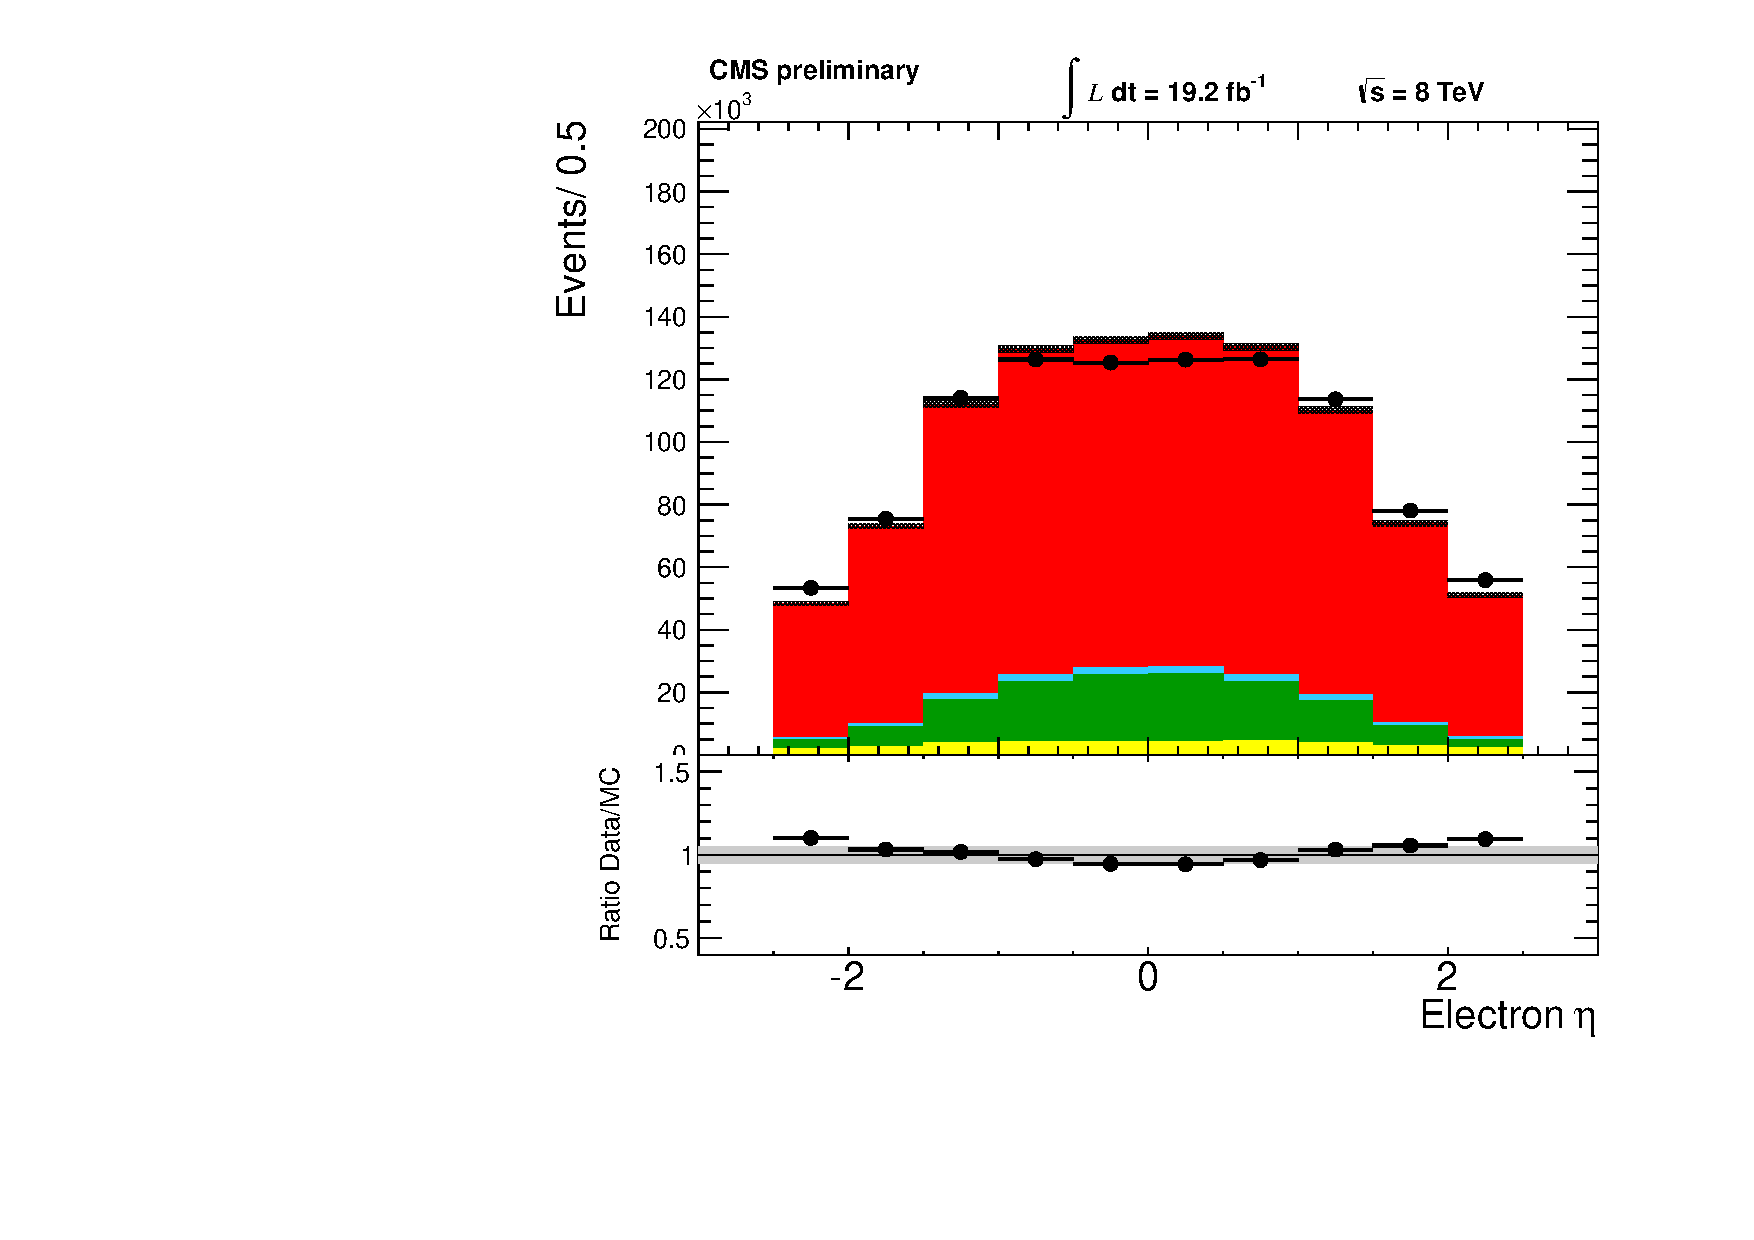
\includegraphics[width=0.49\textwidth]{plots/2012_DataMC/el_W_electron_eta.pdf}
    \caption{Comparison of the electron $E_{T} $ (left) and the
    electron $\eta $ (right) distributions from data and MC for the
    electron+jets selection. 
    }
   \label{fig:elec_electron}}
\end{figure}
%%%%%%%%%%%%%%%%%%%%%%%%%%%%
\begin{figure}[h!t]
  {\centering
    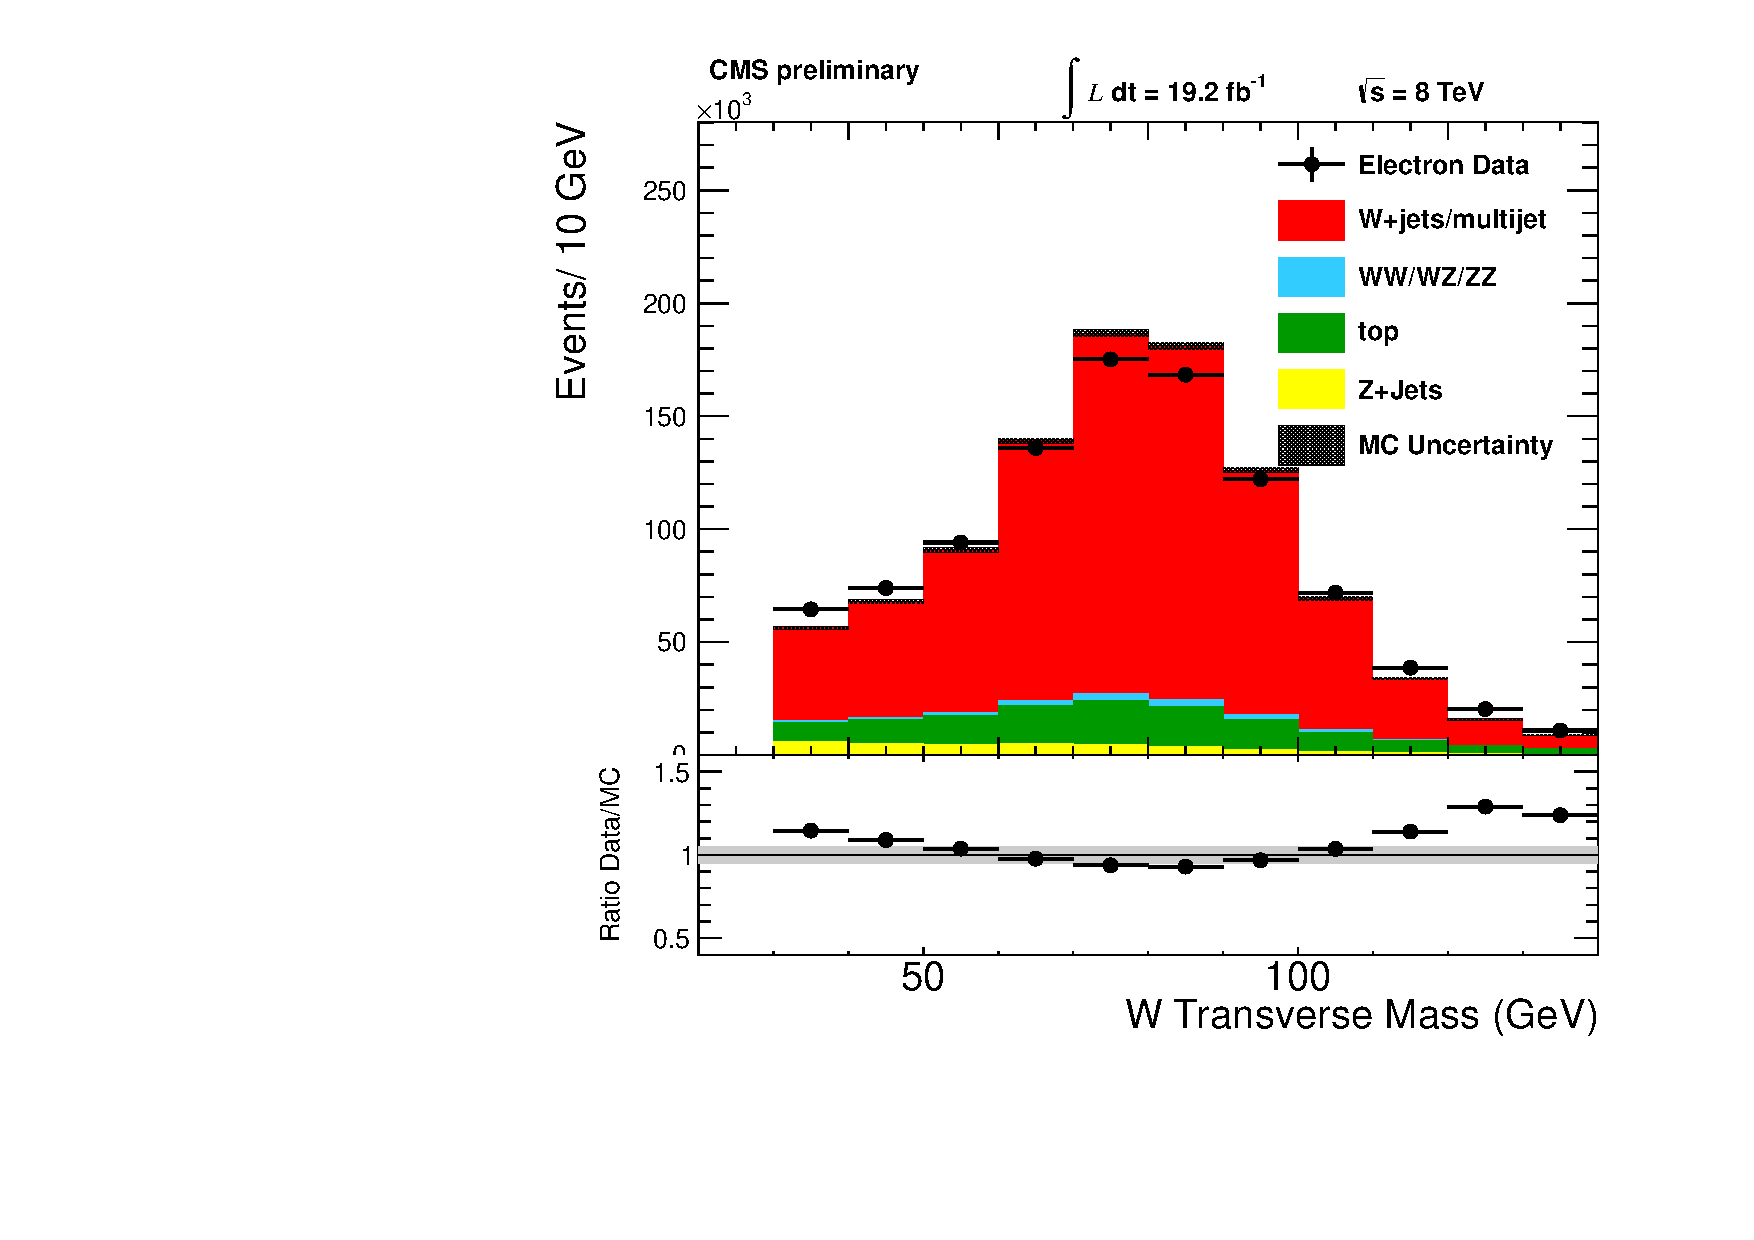
\includegraphics[width=0.49\textwidth]{plots/2012_DataMC/el_W_mt.pdf}
    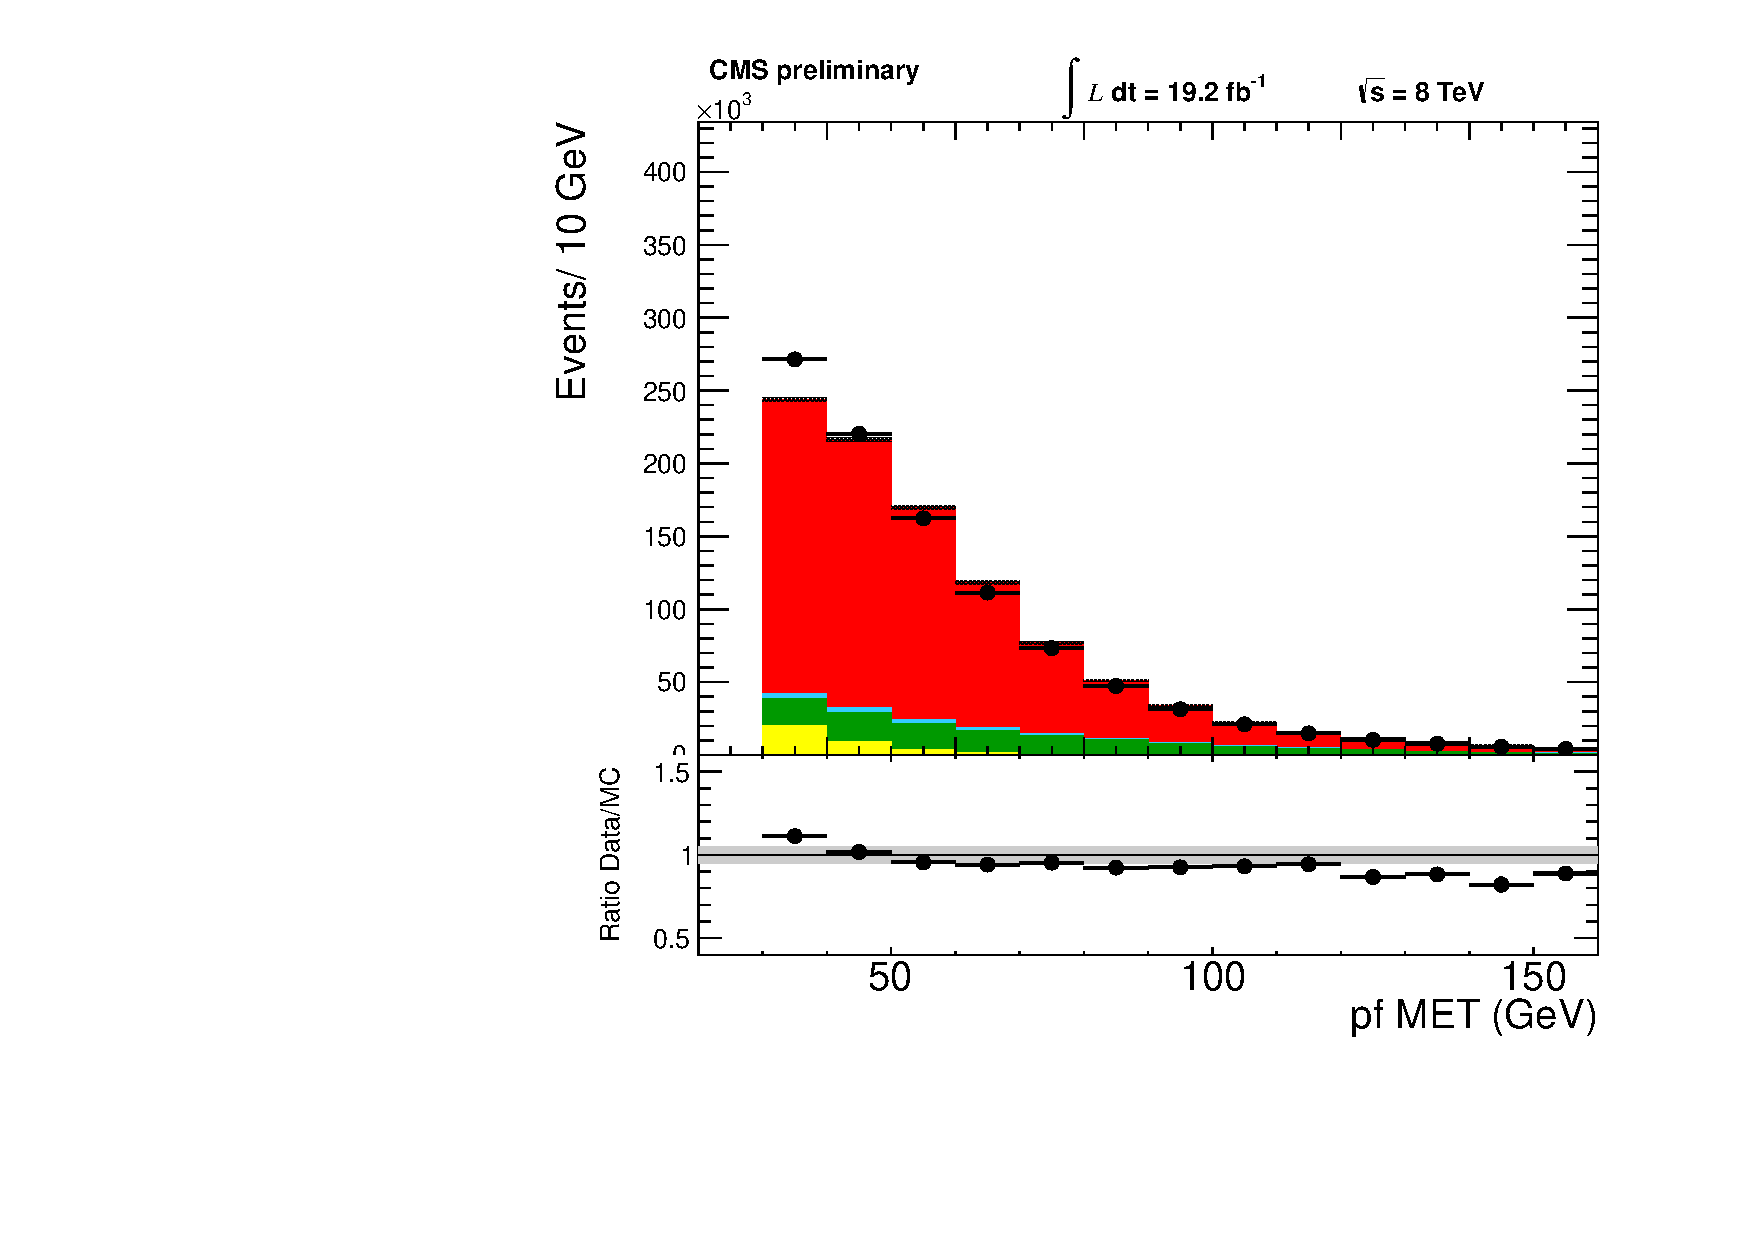
\includegraphics[width=0.49\textwidth]{plots/2012_DataMC/el_event_met_pfmet.pdf}
    \caption{Comparison of the distributions from data and MC of the transverse mass
     of electron / MET system (left) and the MET (right) for the
      electron+jets selection. 
      }
    \label{fig:elec_W_Mt}}
\end{figure}
%%%%%%%%%%%%%%%%%%%%%%%%%%%%
\begin{figure}[h!t]
  {\centering
    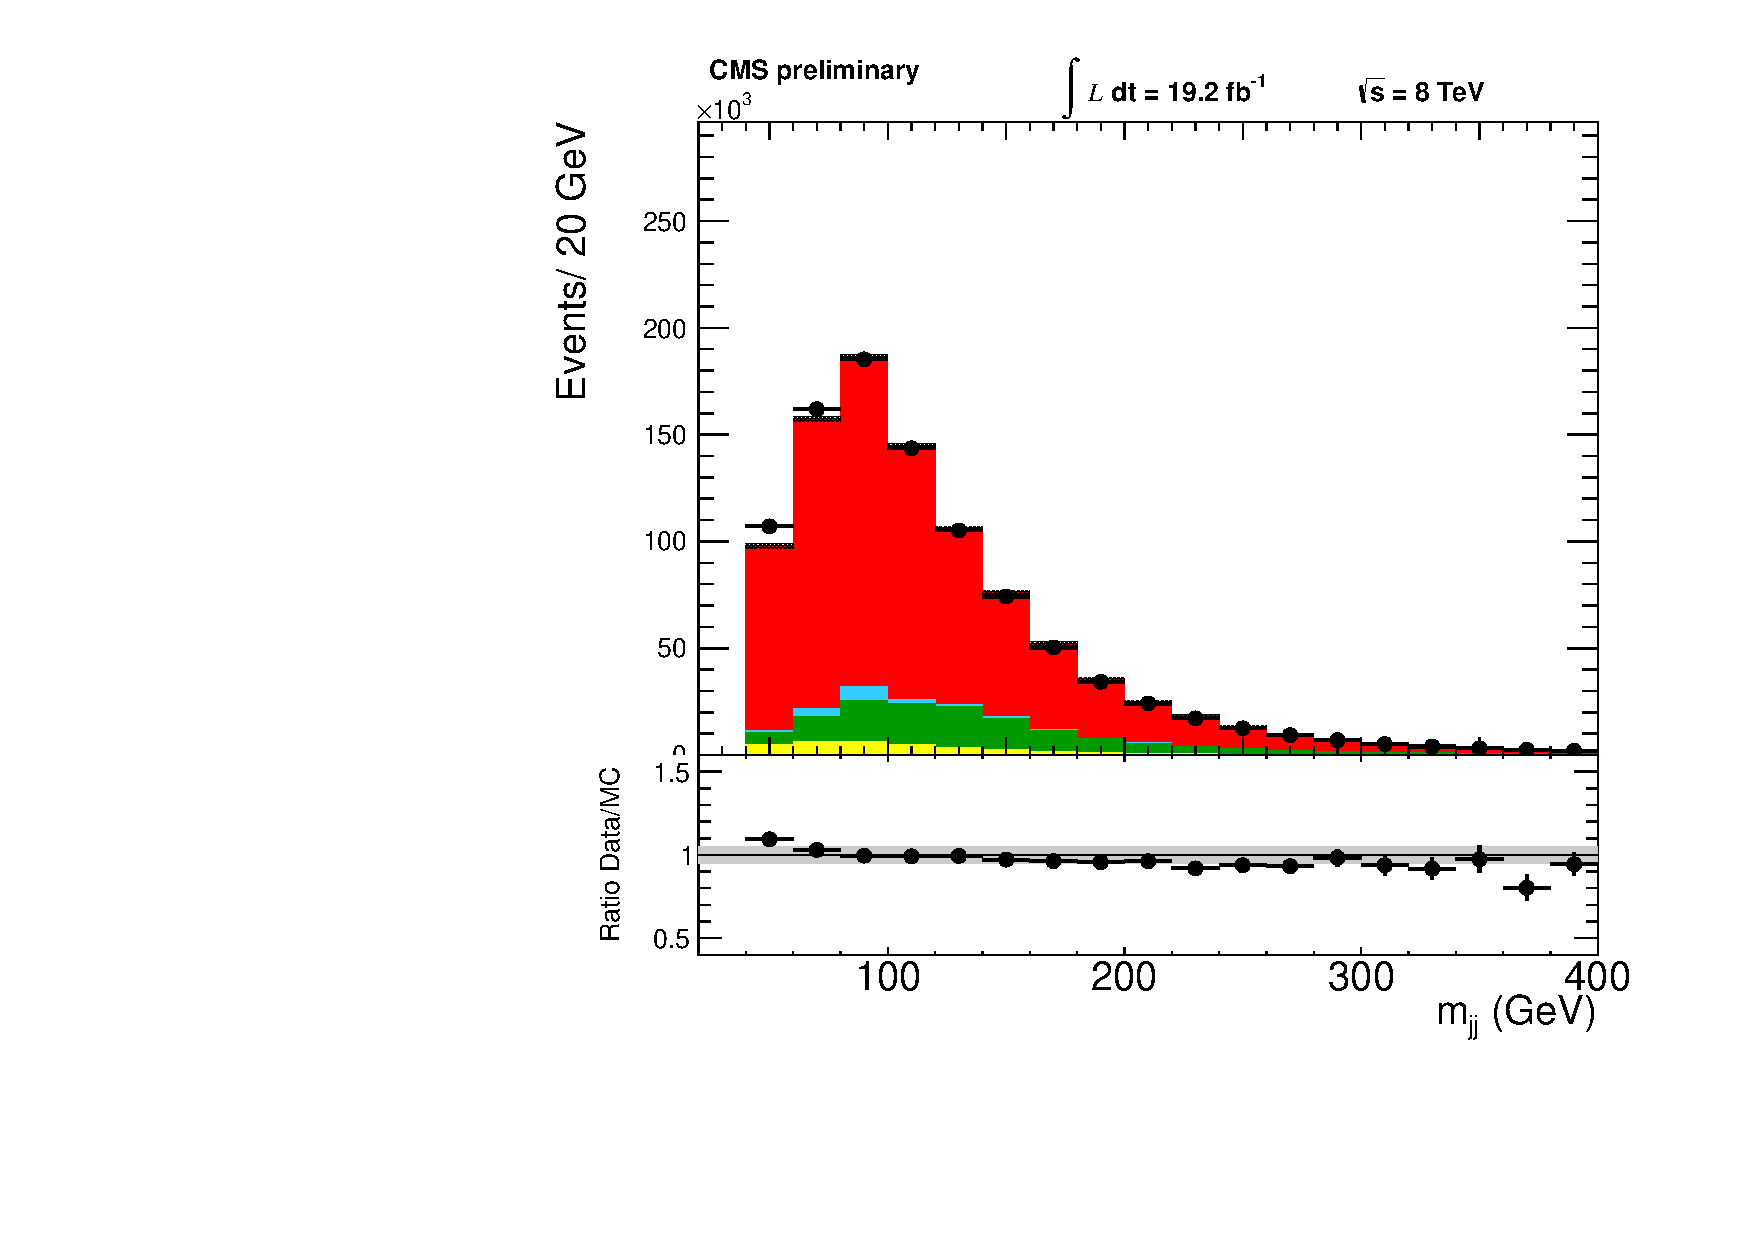
\includegraphics[width=0.49\textwidth]{plots/2012_DataMC/el_mjj.pdf}
    \caption{Comparison of the dijet mass ($m_{JJ}$) distributions from data and MC for 
      the electron+jets selection. }
    \label{fig:elec_mjj}}
\end{figure}
%%%%%%%%%%%%%%%%%%%%%%%%%%%%
%%%%%%%%%%%%%%%%%%%%%%%%%%%%
\clearpage
The data MC comparison for the various inputs to the MVA are shown in  
Figures ~\ref{fig:mu_theta}-\ref{fig:mu_ww}
for the muon+jets sample and in 
Figures ~\ref{fig:elec_theta}-\ref{fig:elec_ww} for
the electron+jets sample. 

% quark-gluon discriminants
%% %%%%%%%%%%%%%%%%%%%%%%%%%%%%
%% \begin{figure}[h!t]
%%   {\centering
%%     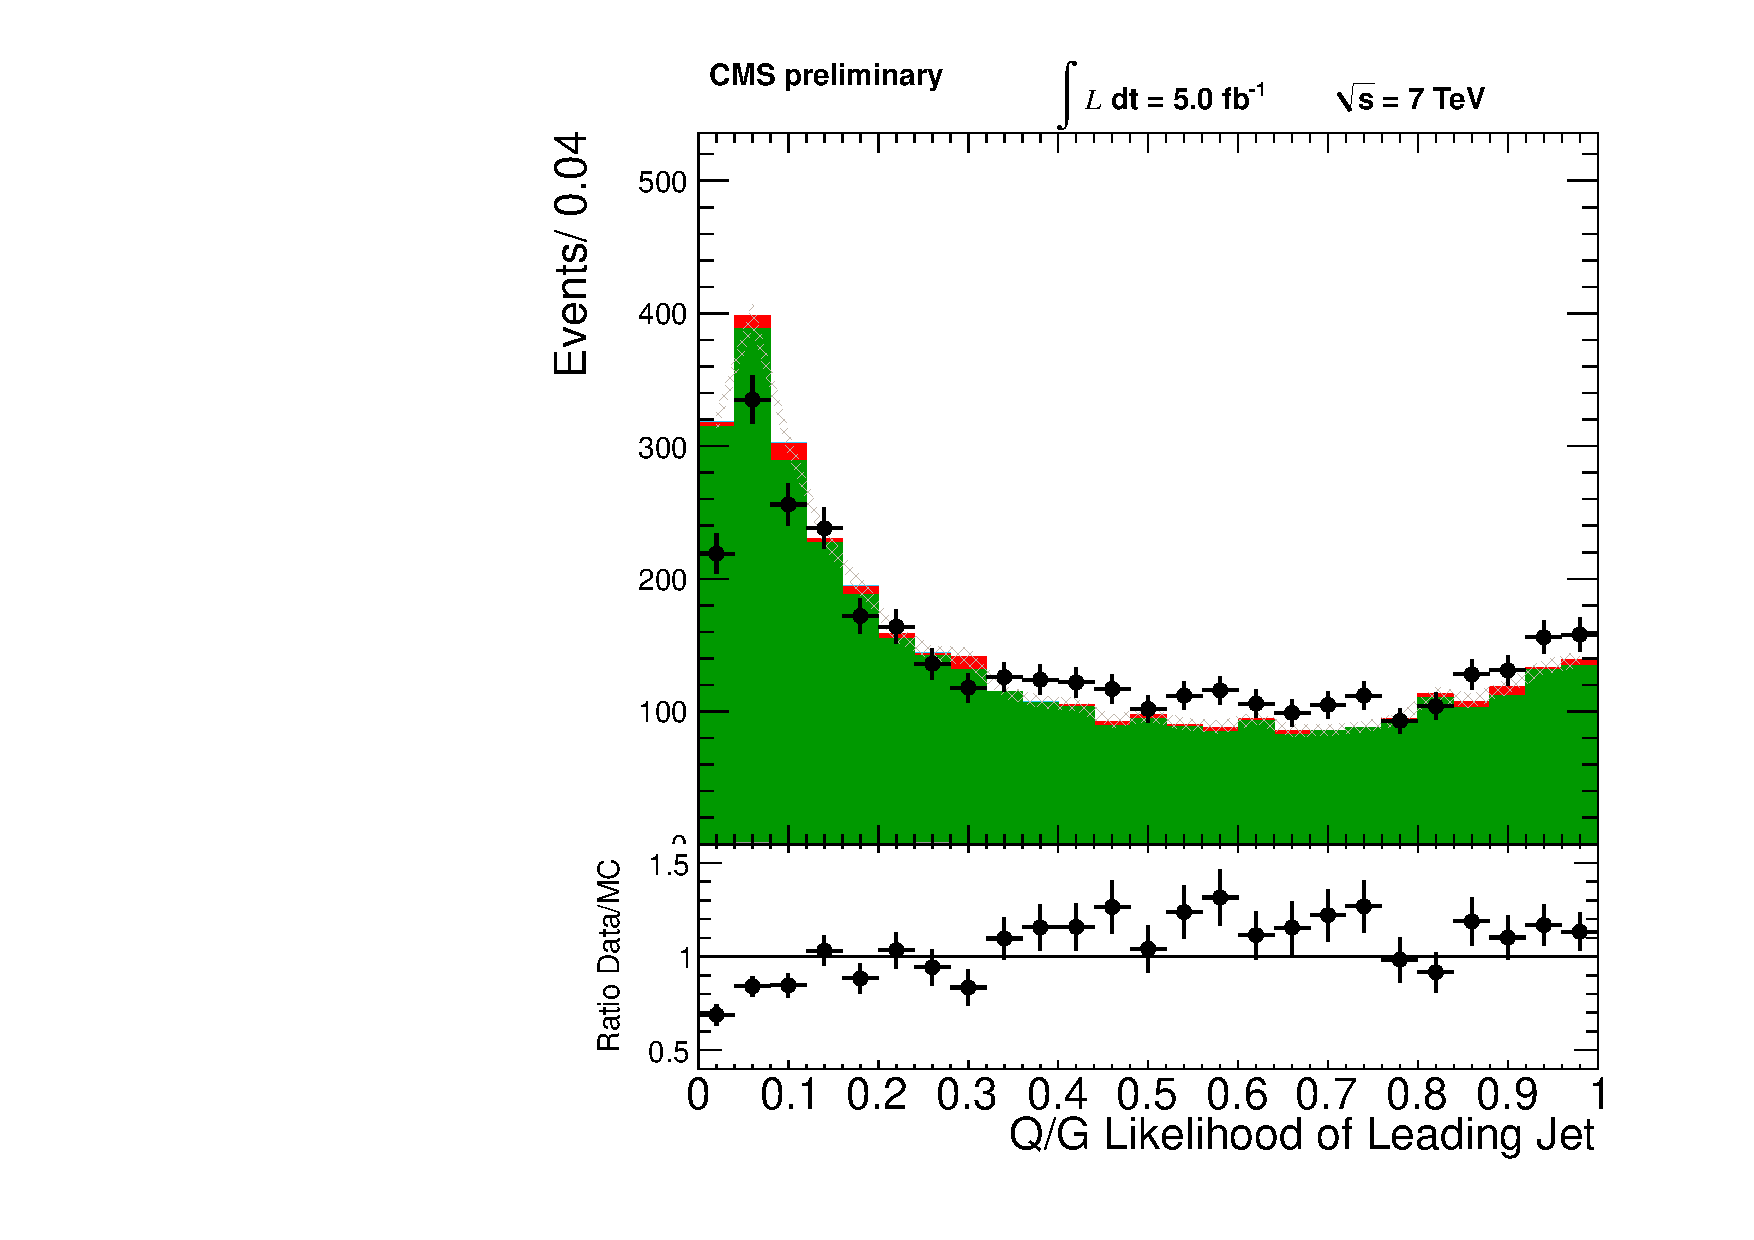
\includegraphics[width=0.49\textwidth]{plots/2012_DataMC/mu_jetld_qgl.pdf}
%%     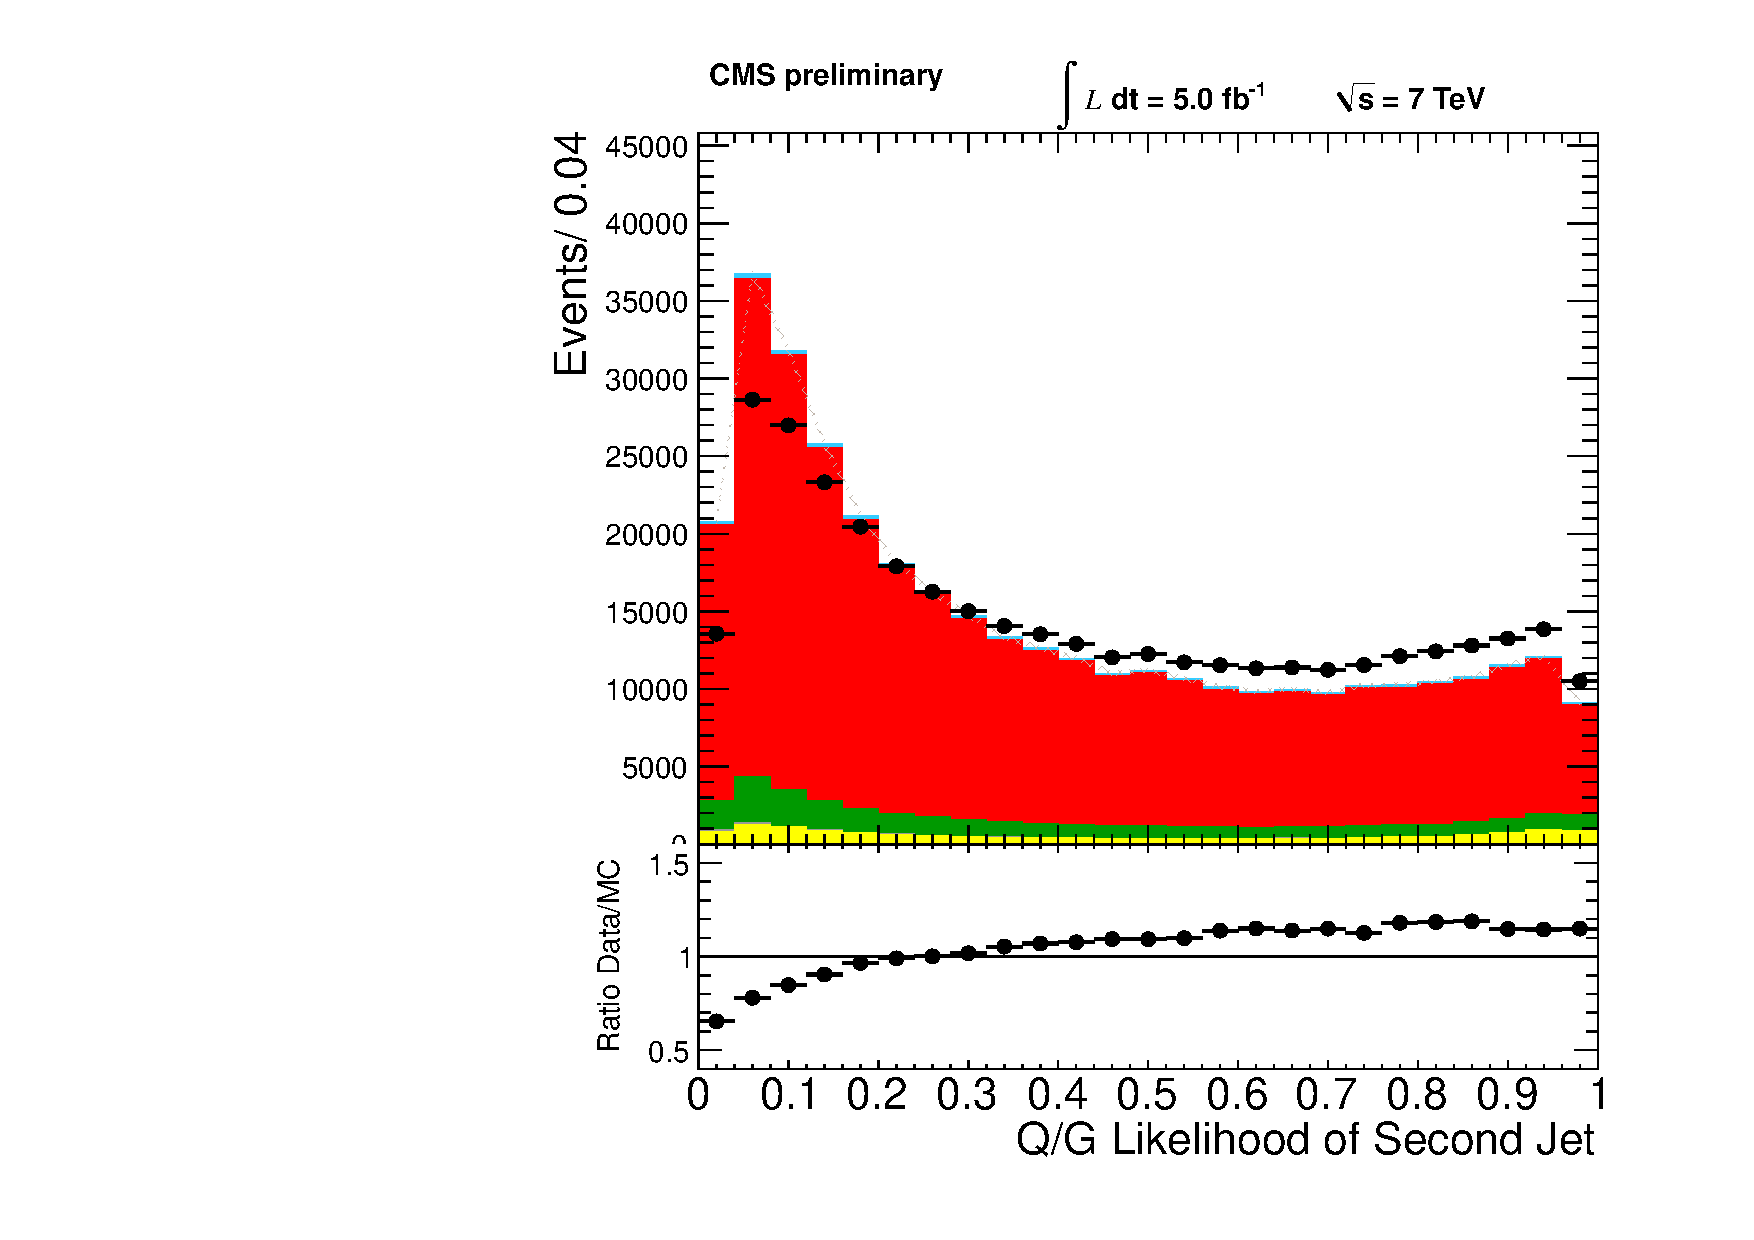
\includegraphics[width=0.49\textwidth]{plots/2012_DataMC/mu_jetnt_qgl.pdf}
%%     \caption{Comparison of the Quark-gluon likelihood distributions for leading jet (left)
%%     second leading (right) from data and MC for the muon+jets selection.}
%% \label{fig:mu_jet_qgl}}
%% \end{figure}
% angular variables
%%%%%%%%%%%%%%%%%%%%%%%%%%%%
\begin{figure}[h!t]
  {\centering
    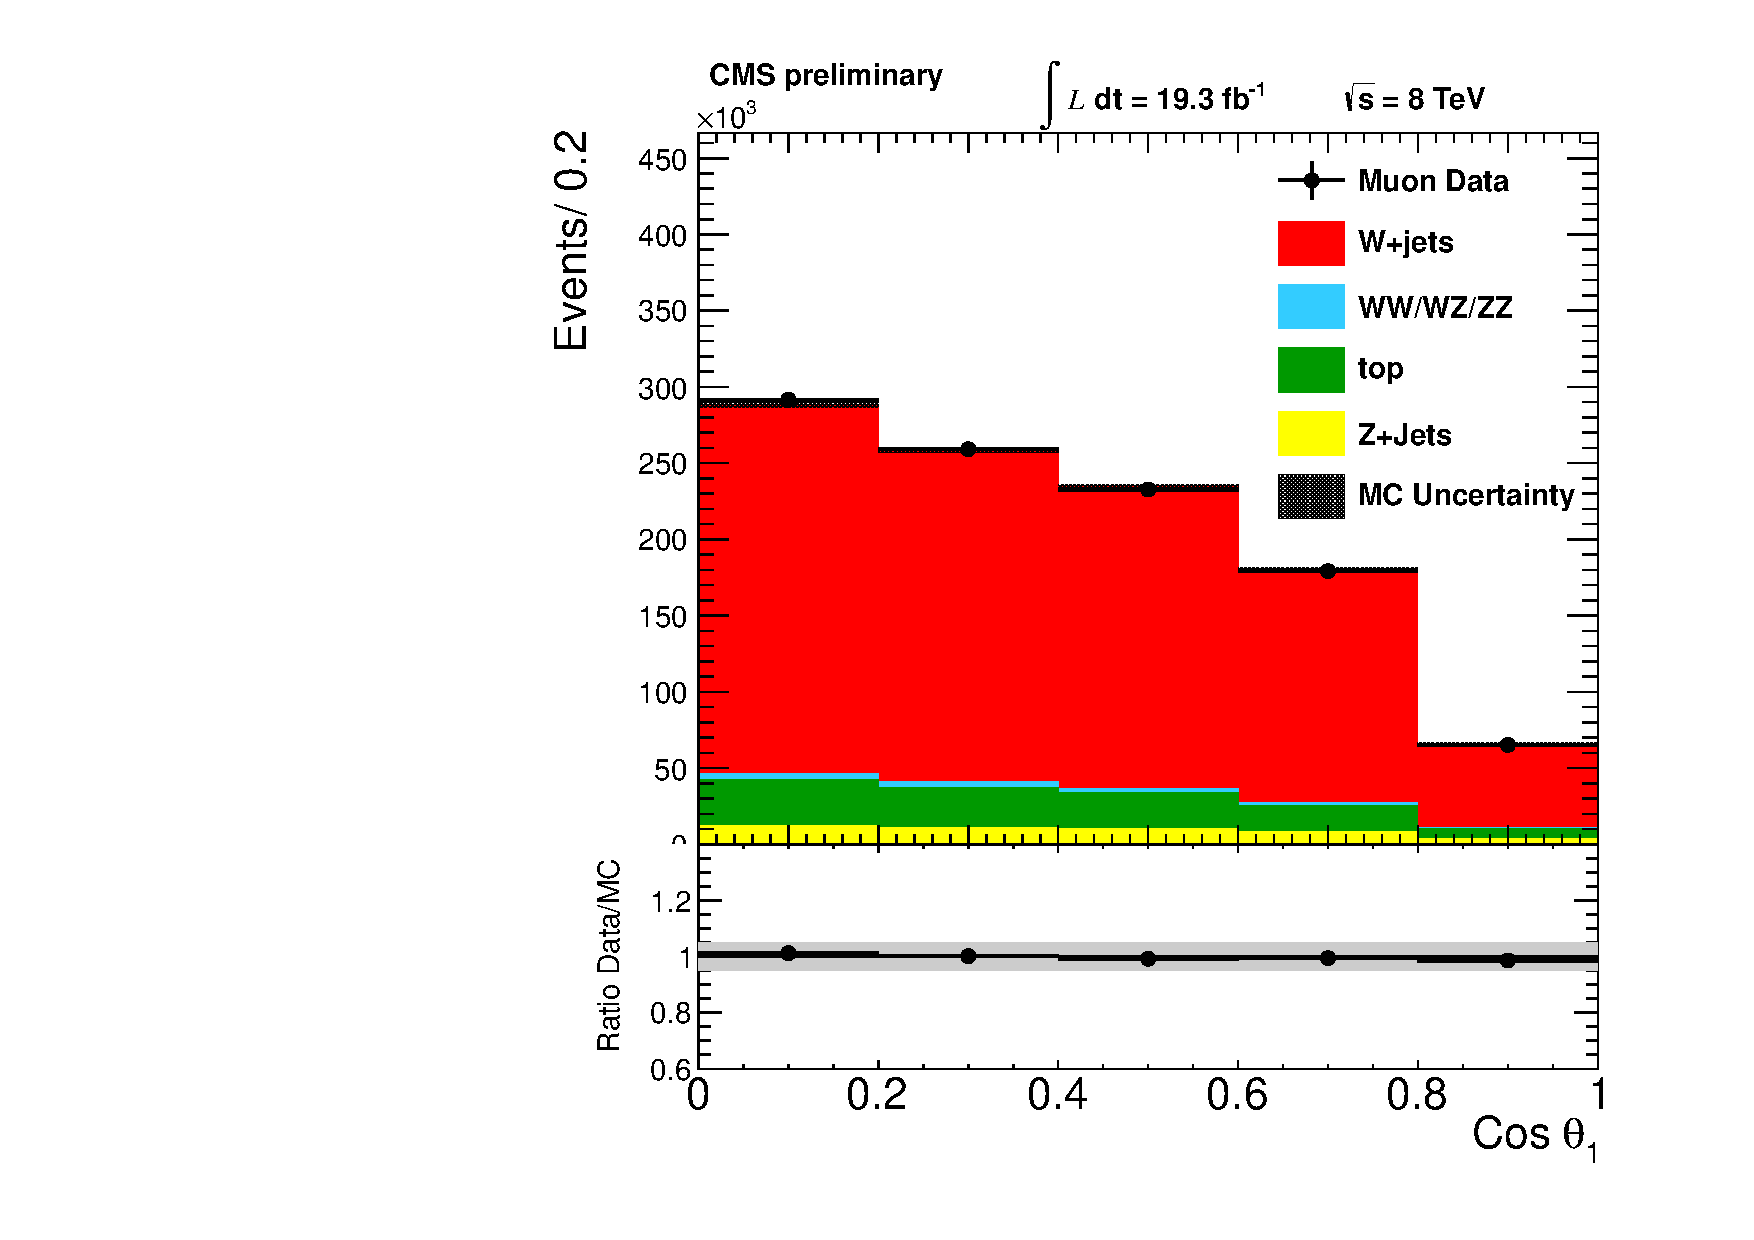
\includegraphics[width=0.49\textwidth]{plots/2012_DataMC/mu_ha.pdf}
    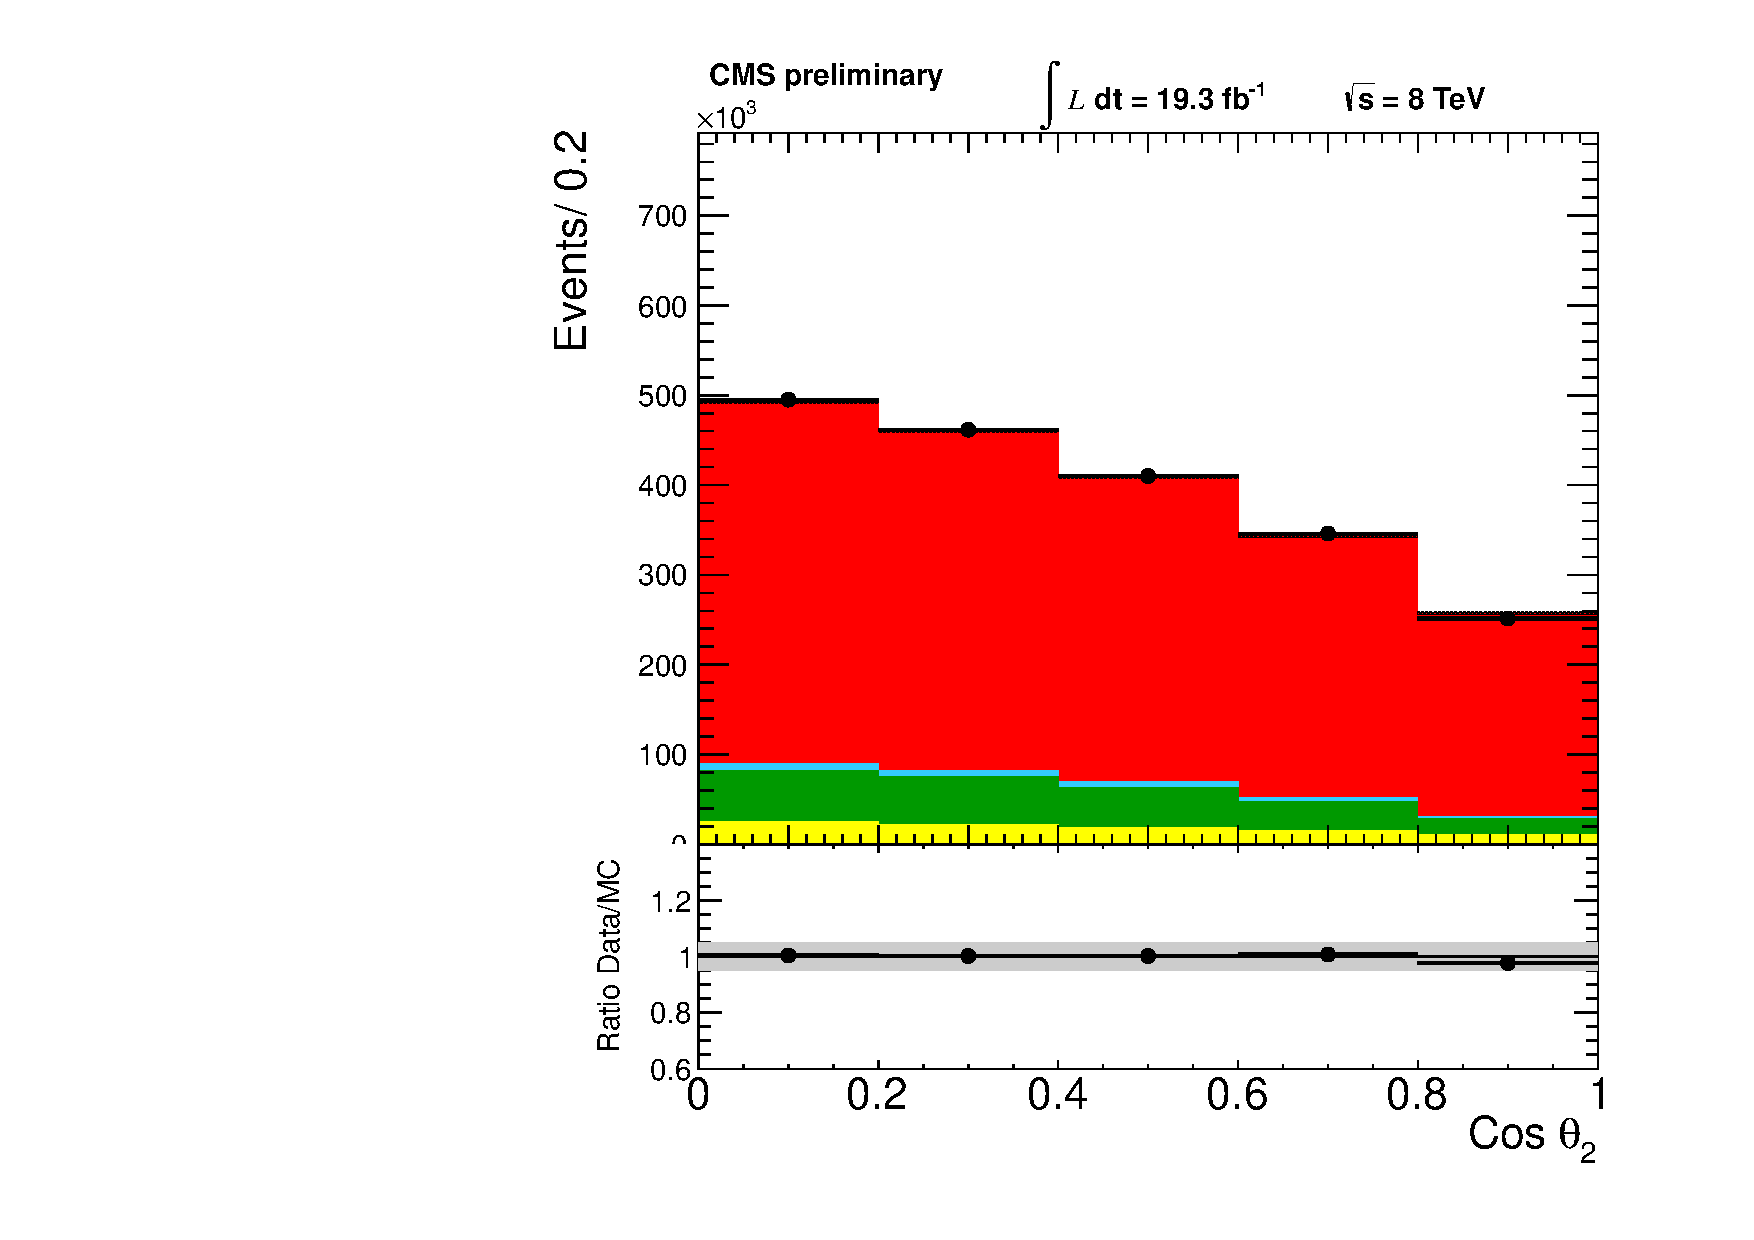
\includegraphics[width=0.49\textwidth]{plots/2012_DataMC/mu_hb.pdf}
    \caption{Comparison of the angular distributions for $\cos\theta_{1}$ (left) and
   $\cos\theta_{2}$ (right) from data and MC for the muon+jets selection.}
\label{fig:mu_theta}}
\end{figure}
%%%%%%%%%%%%%%%%%%%%%%%%%%%%
\begin{figure}[h!t]
  {\centering
     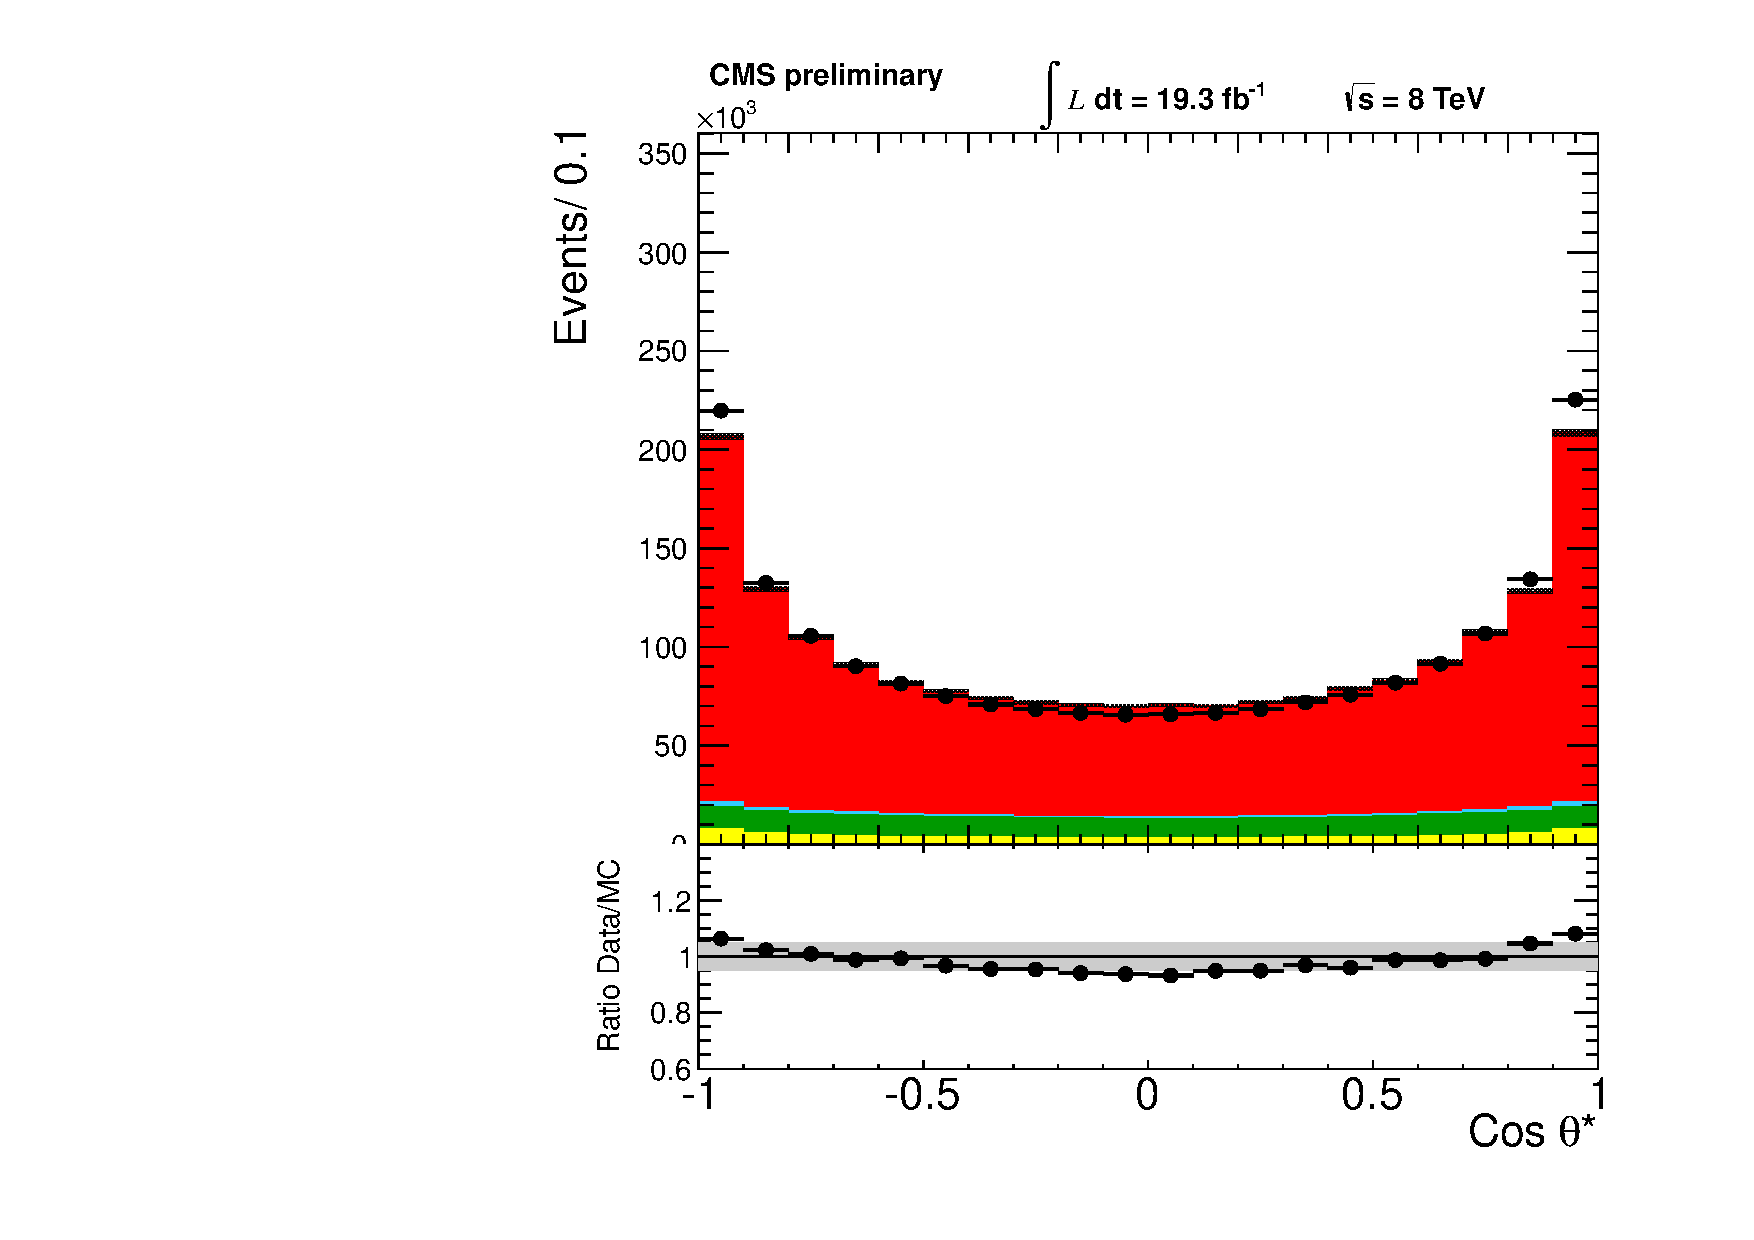
\includegraphics[width=0.49\textwidth]{plots/2012_DataMC/mu_hs.pdf}
    \caption{Comparison of the angular distributions for $\cos\theta^{\ast}$ from data and MC 
   for the muon+jets selection.}
\label{fig:mu_thetas}}
\end{figure}
%%%%%%%%%%%%%%%%%%%%%%%%%%%%
\begin{figure}[h!t]
  {\centering
    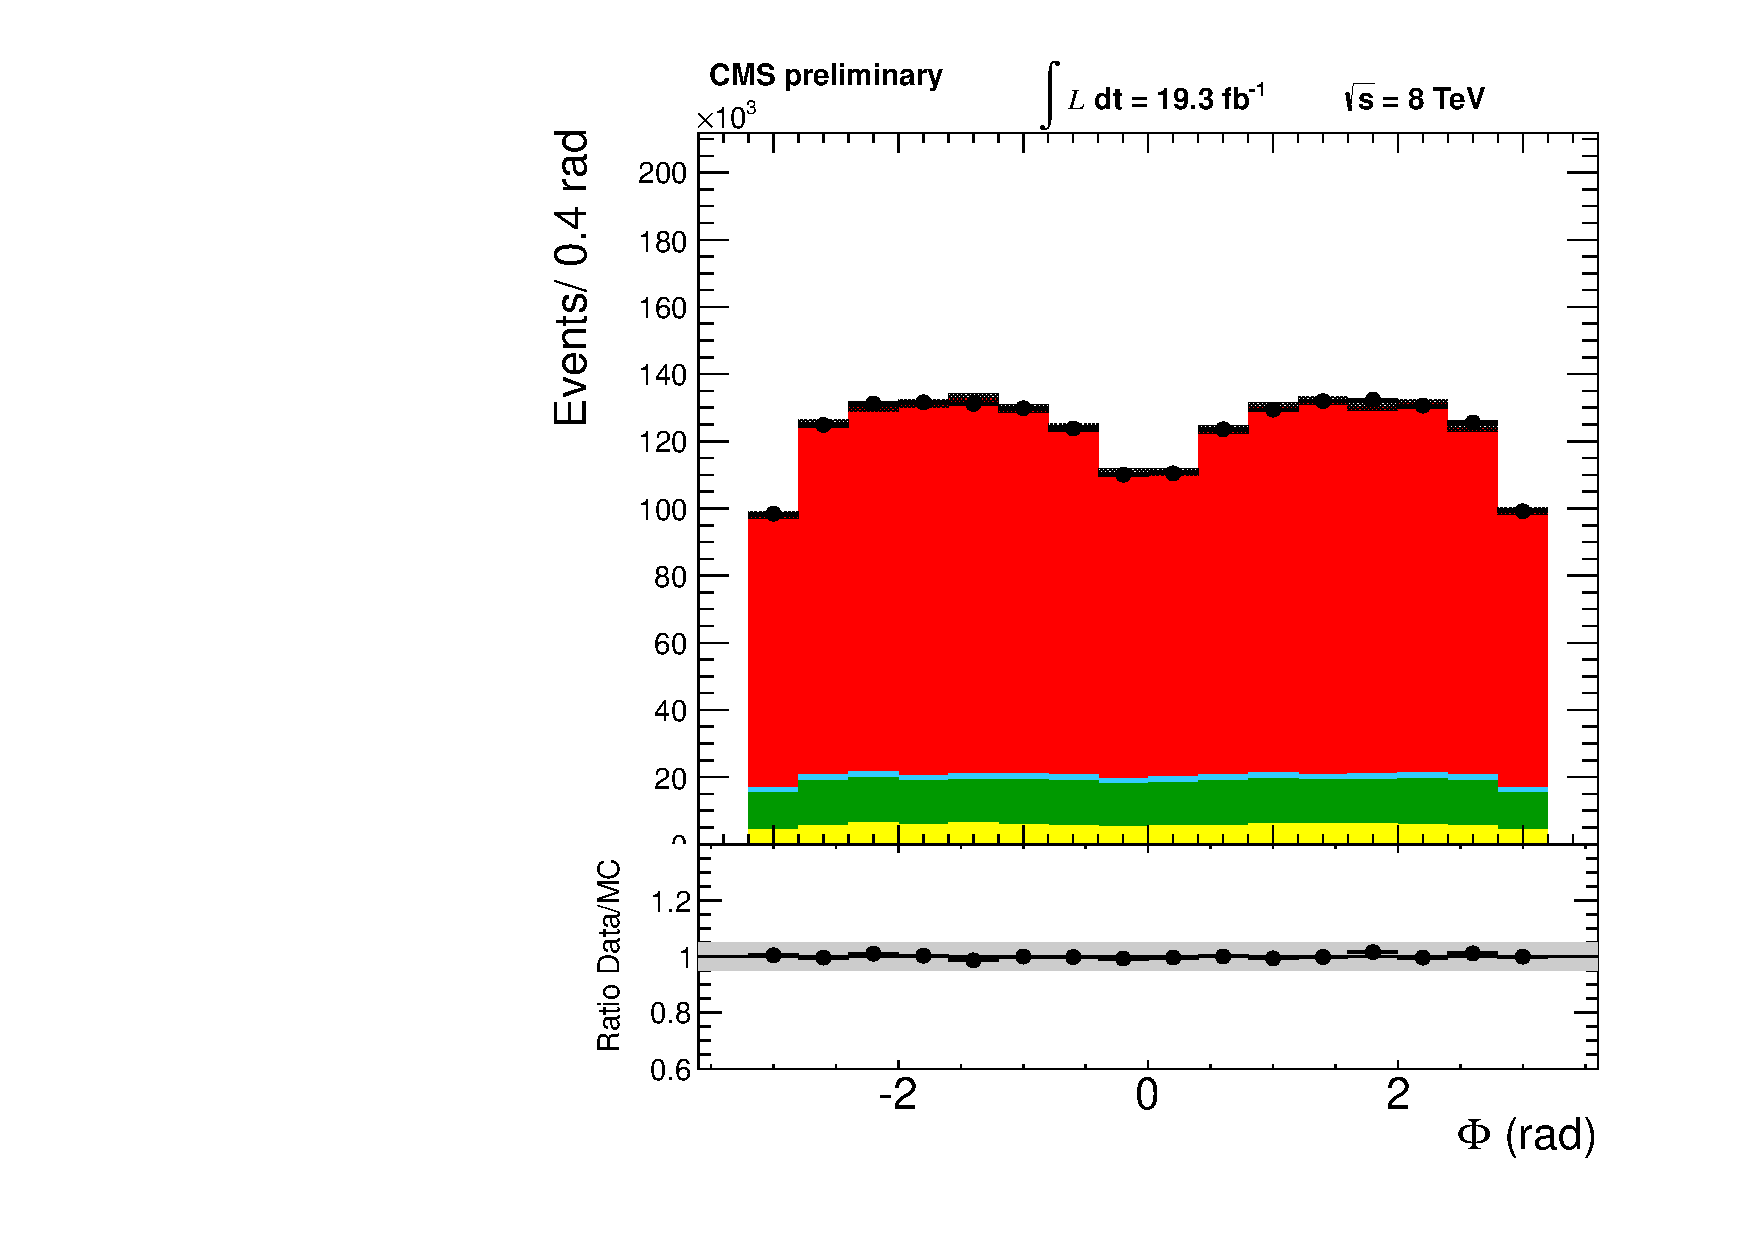
\includegraphics[width=0.49\textwidth]{plots/2012_DataMC/mu_phi.pdf}
    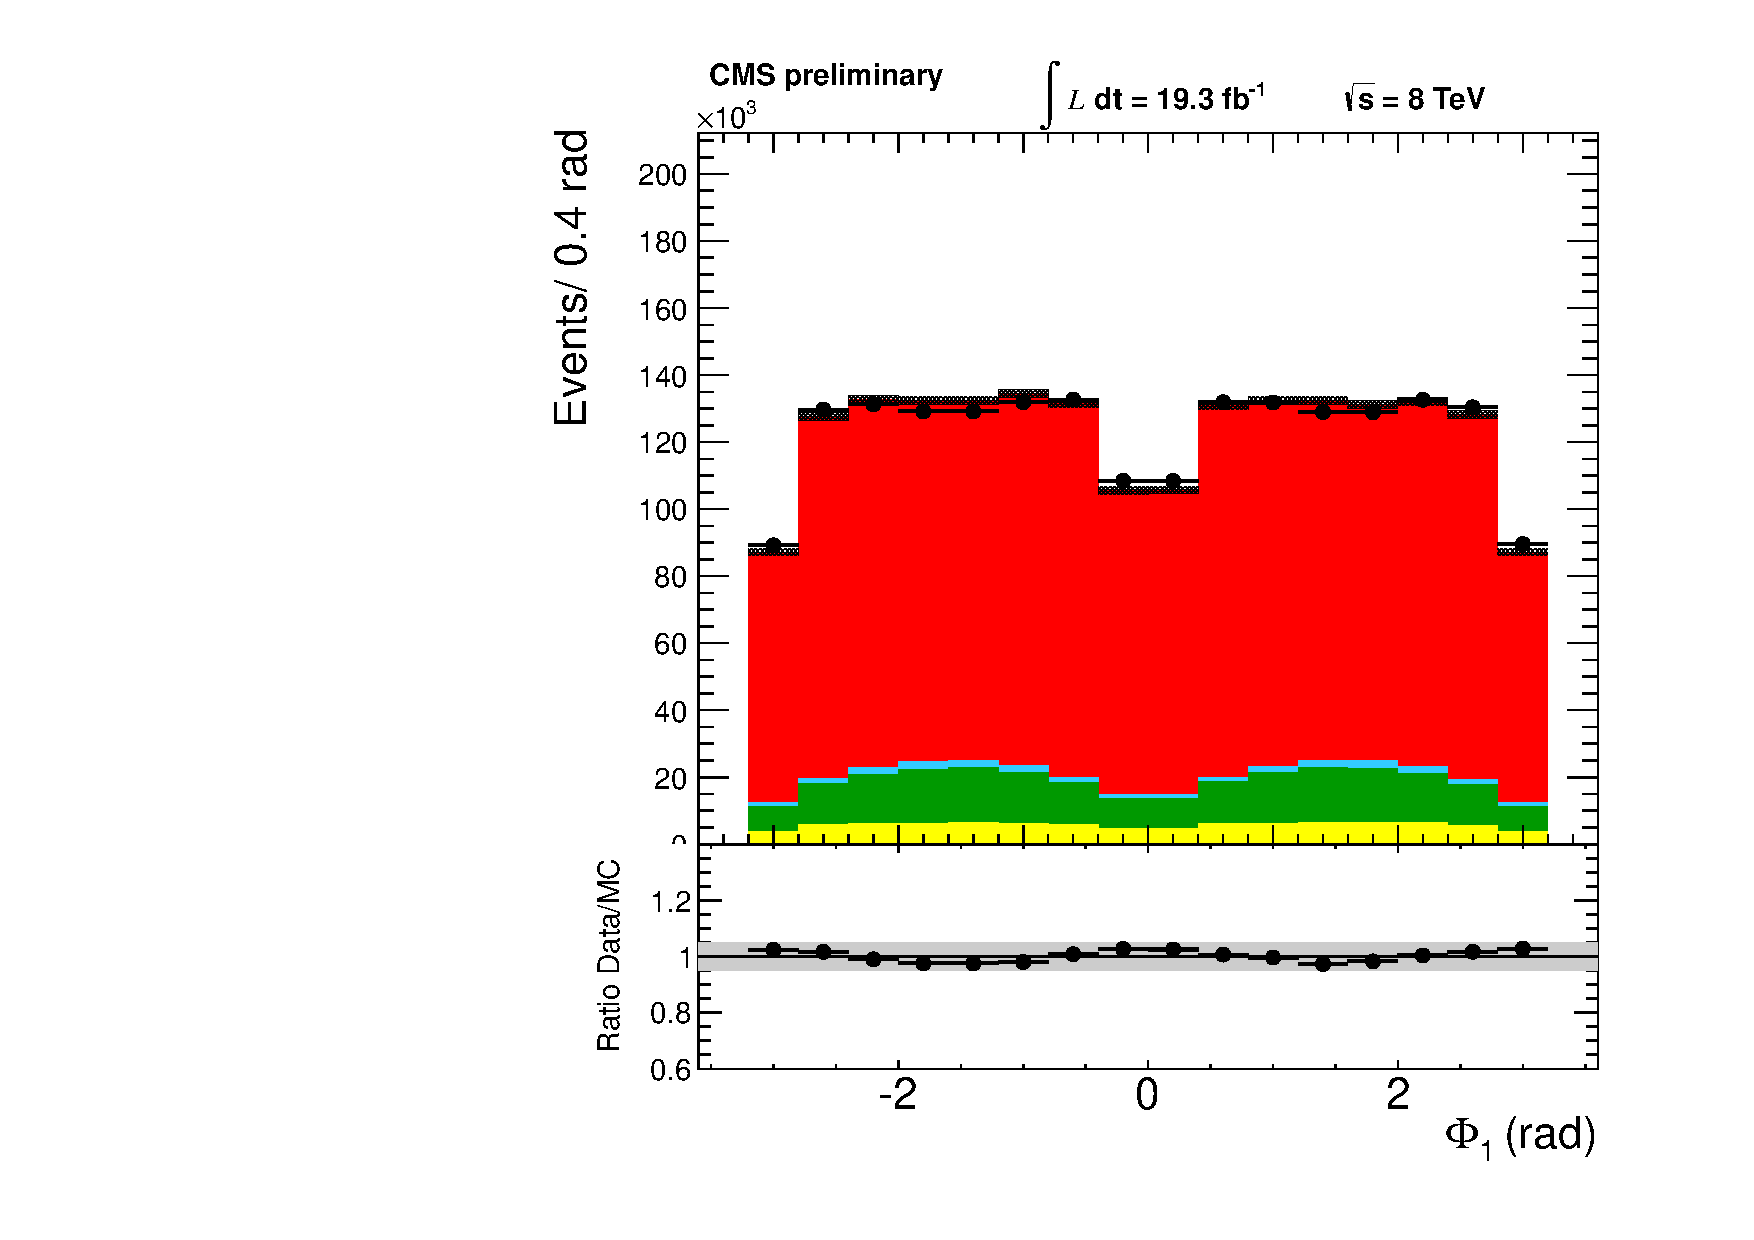
\includegraphics[width=0.49\textwidth]{plots/2012_DataMC/mu_phib.pdf}
    \caption{Comparison of the angular distributions for $\Phi$ (left) and $\Phi_{1}$ (right) from data and 
      MC for the muon+jets selection.}
\label{fig:mu_phi}}
\end{figure}

%%%%%%%%%%%%%%%%%%%%%%%%%%%%
\begin{figure}[h!t]
  {\centering
    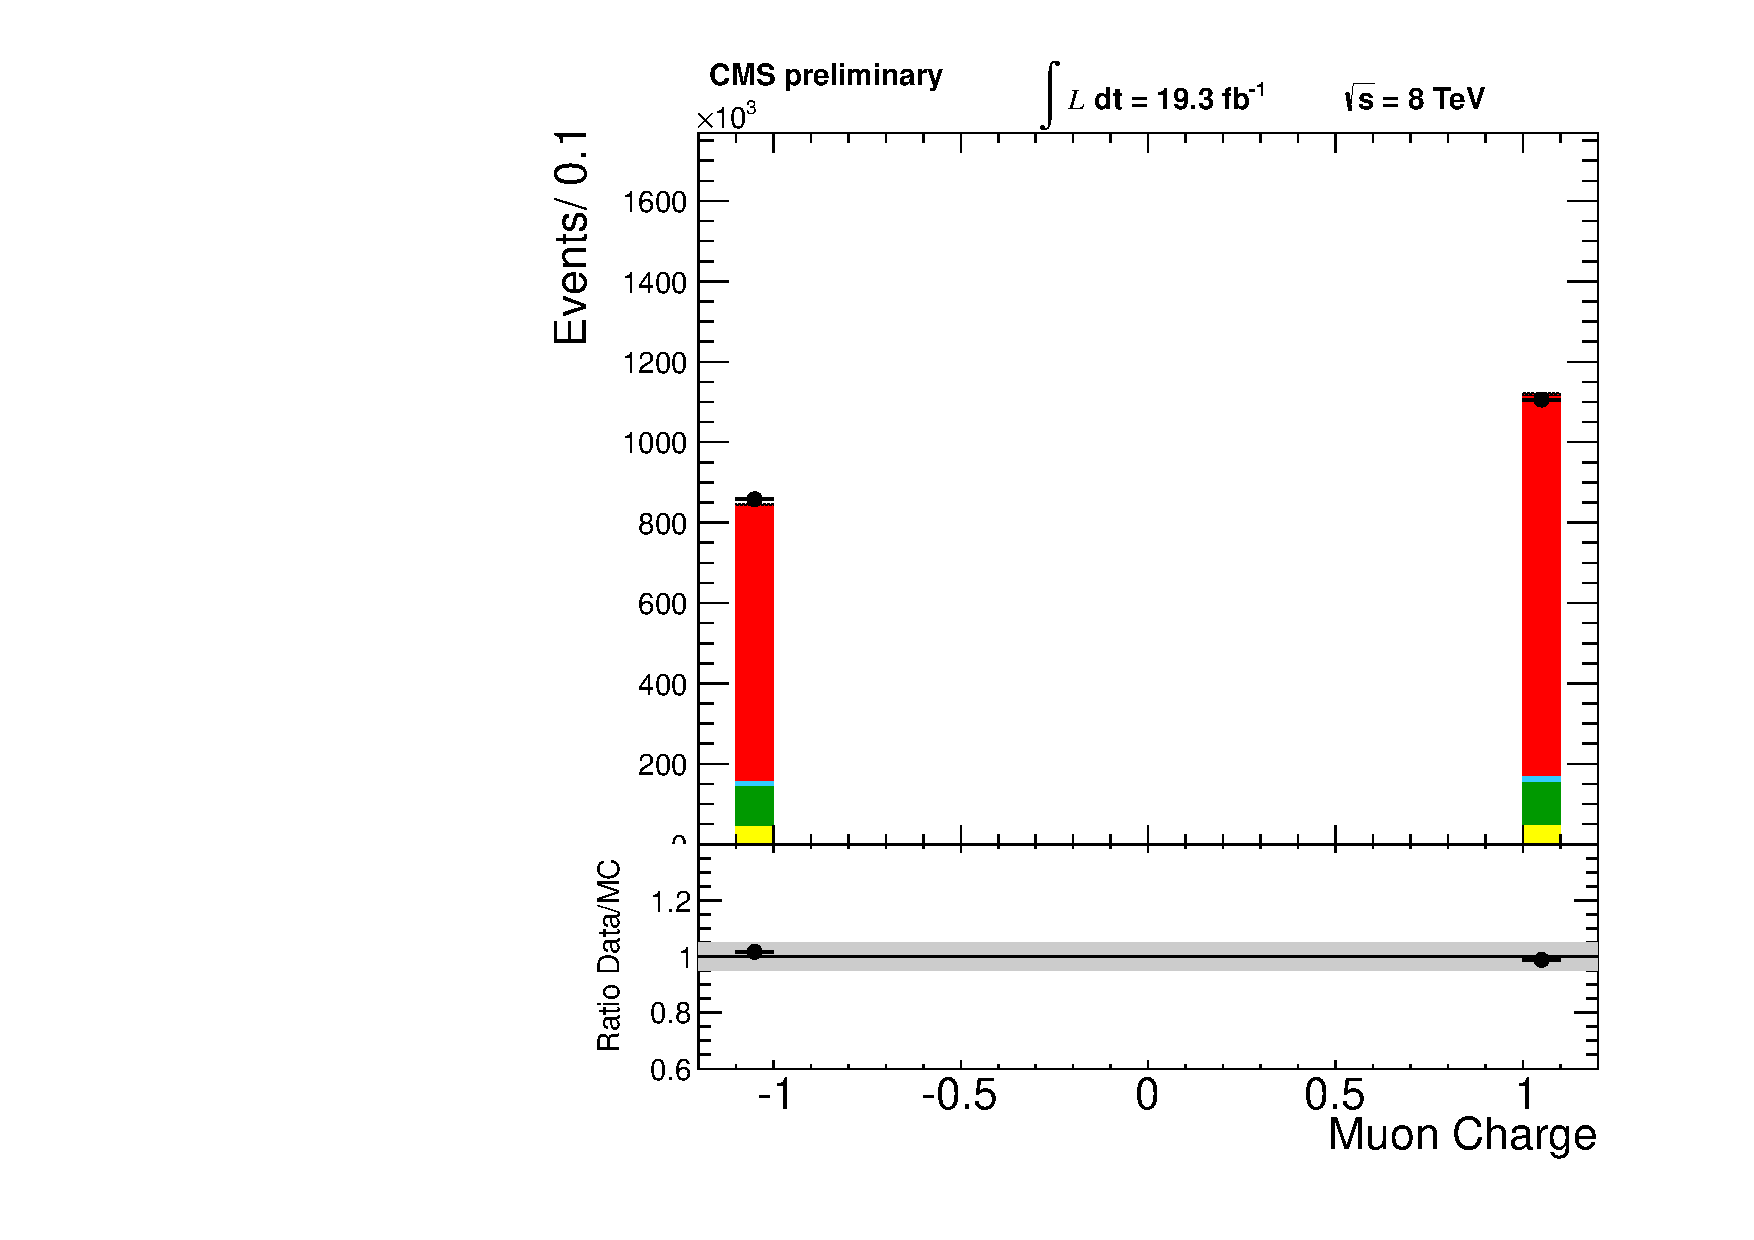
\includegraphics[width=0.49\textwidth]{plots/2012_DataMC/mu_charge.pdf}
    \caption{Comparison of the charge of the muon from data and MC for the muon+jets selection.}
\label{fig:mu_chg}}
\end{figure}

% rapidity and pt of the WW system

%%%%%%%%%%%%%%%%%%%%%%%%%%%%
\begin{figure}[h!t]
  {\centering
    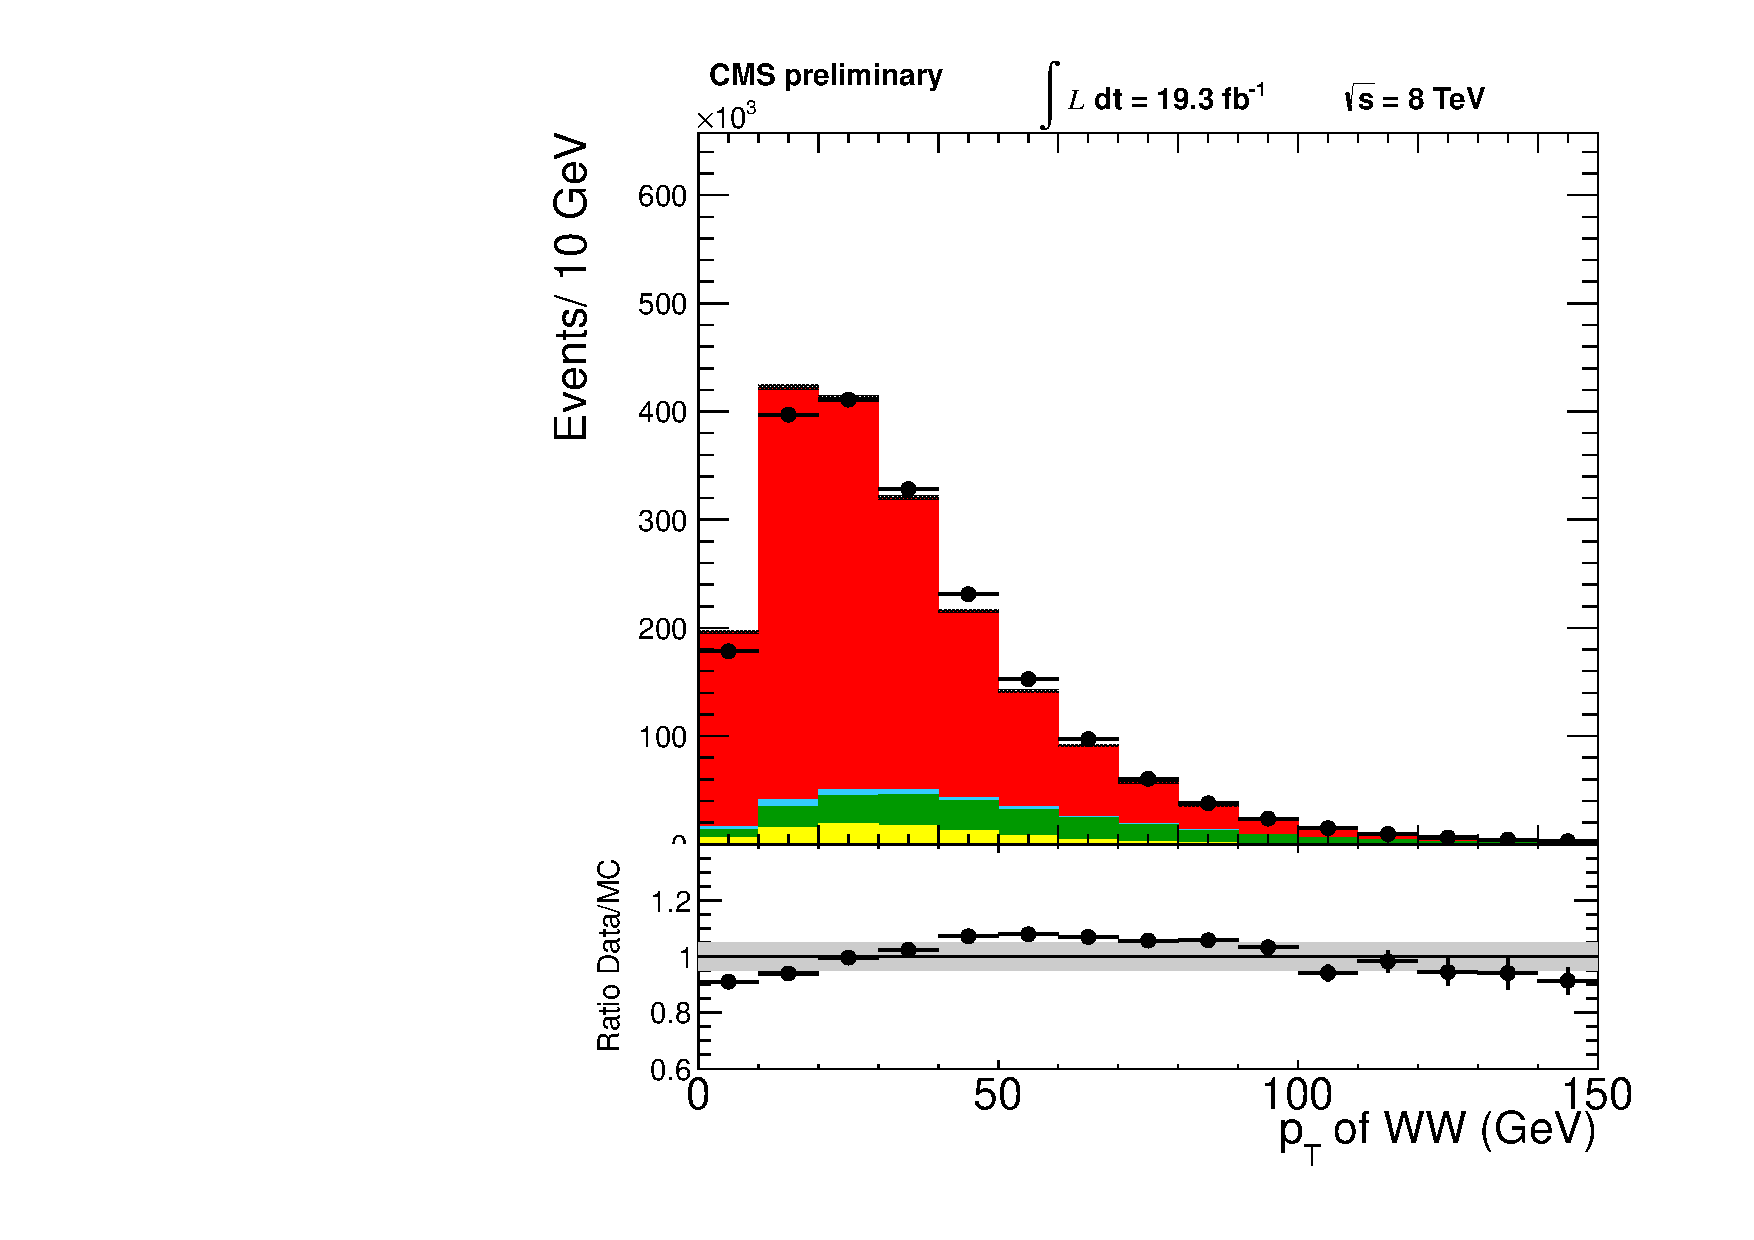
\includegraphics[width=0.49\textwidth]{plots/2012_DataMC/mu_ptlvjj.pdf}
    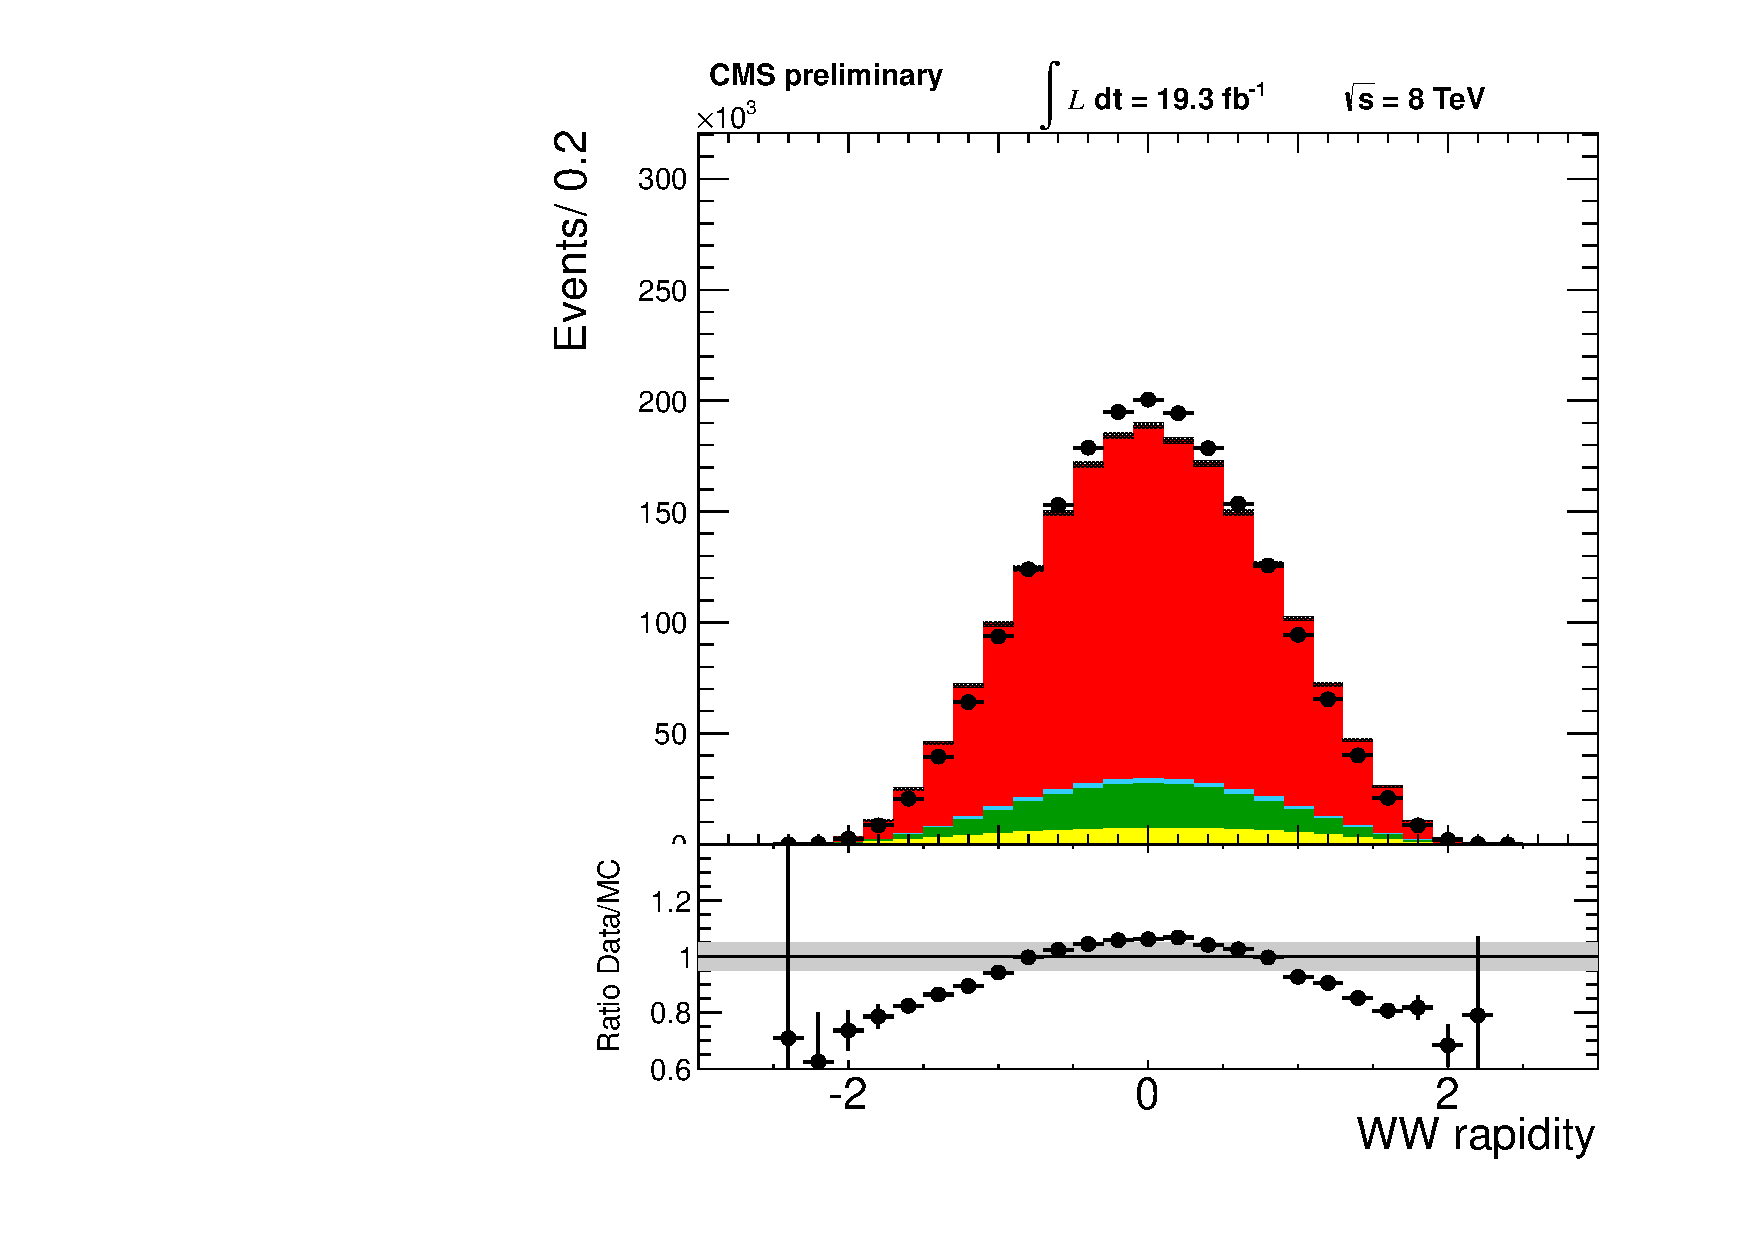
\includegraphics[width=0.49\textwidth]{plots/2012_DataMC/mu_etalvjj.pdf}
    \caption{Comparison of the $p_{T}$ (left) and $\eta$ (right) of the WW system
      from data and MC for the muon+jets selection.}
\label{fig:mu_ww}}
\end{figure}

%%%%%%%%%%%%%%%%%%%%%%%%%%%%%%%%%
%%%%%%%%%%%%%%%%%%%%%%%

% quark-gluon discriminants
%%%%%%%%%%%%%%%%%%%%%%%%%%%%
%% \begin{figure}[h!t]
%%   {\centering
%%     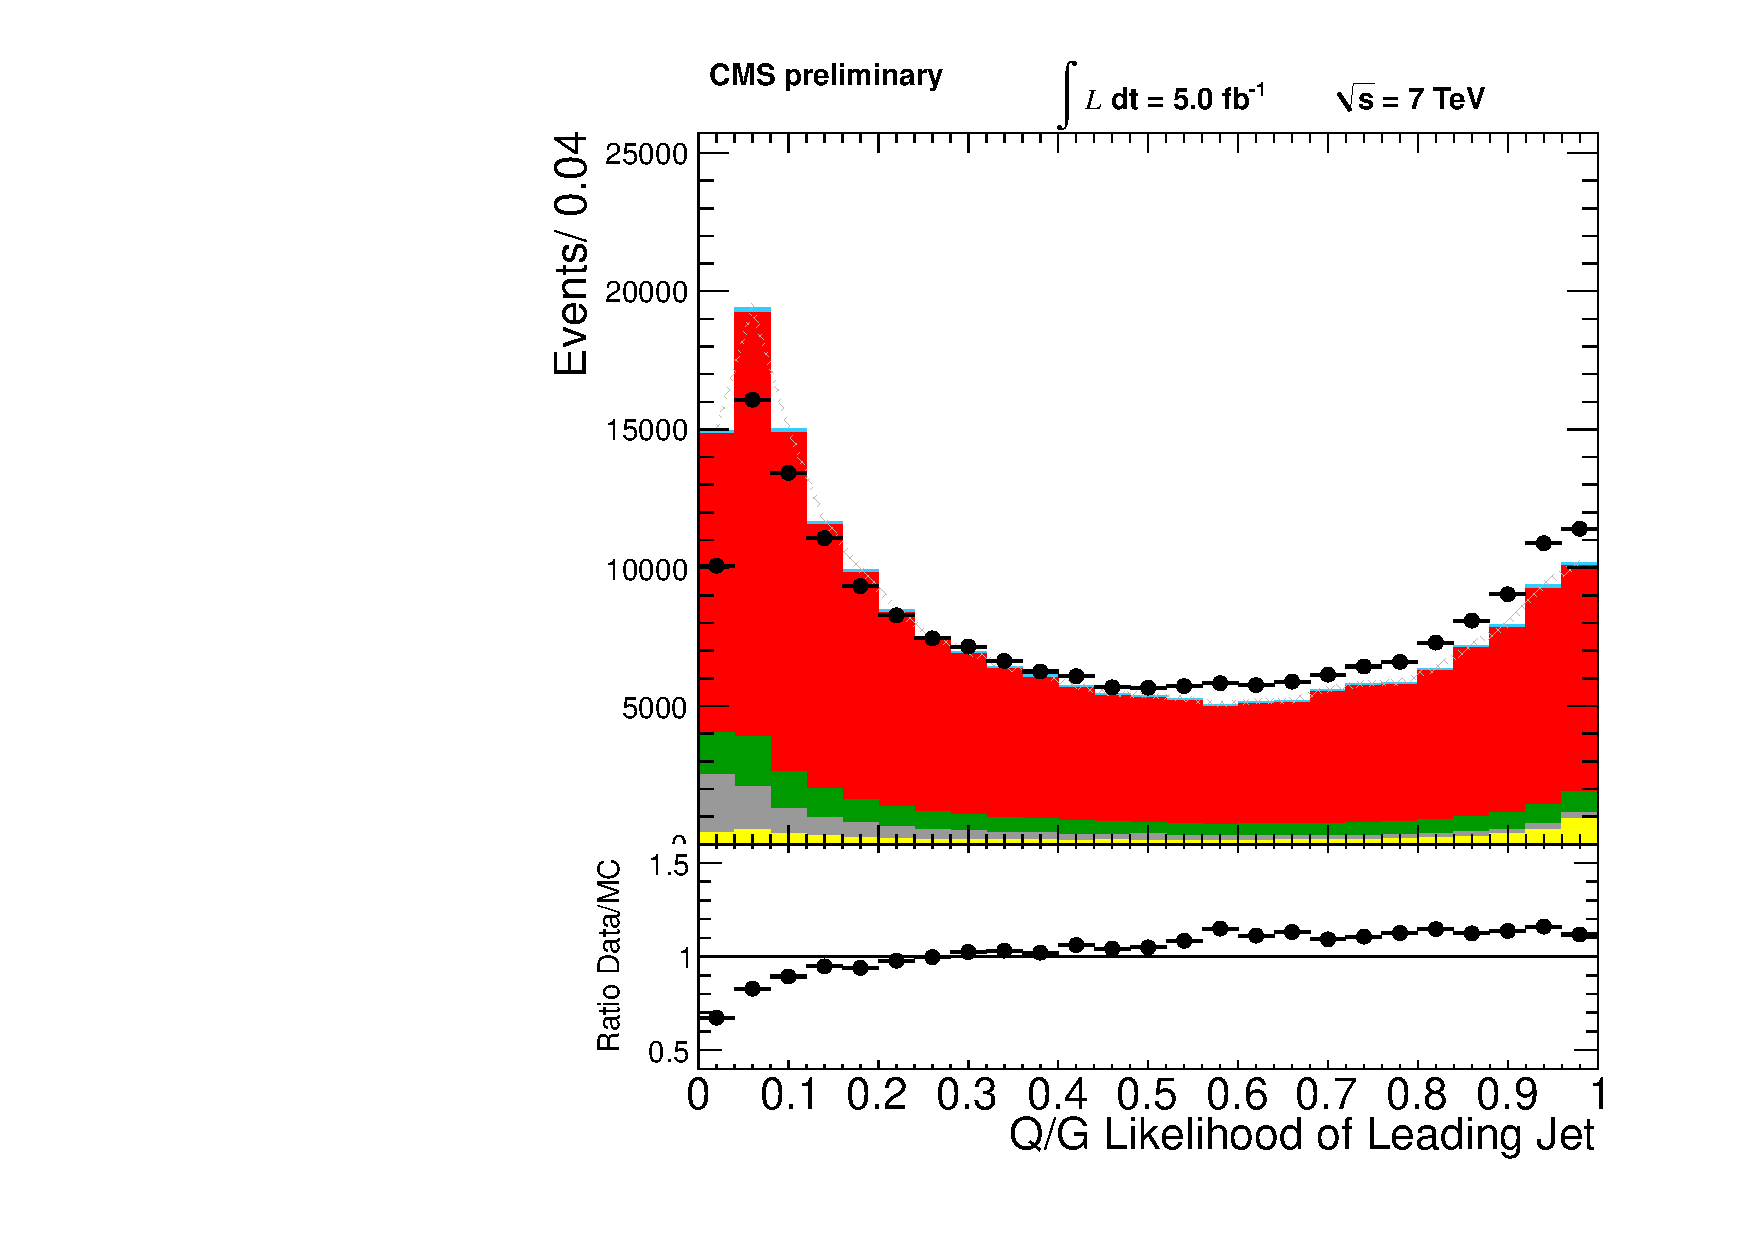
\includegraphics[width=0.49\textwidth]{plots/2012_DataMC/el_jetld_qgl.pdf}
%%     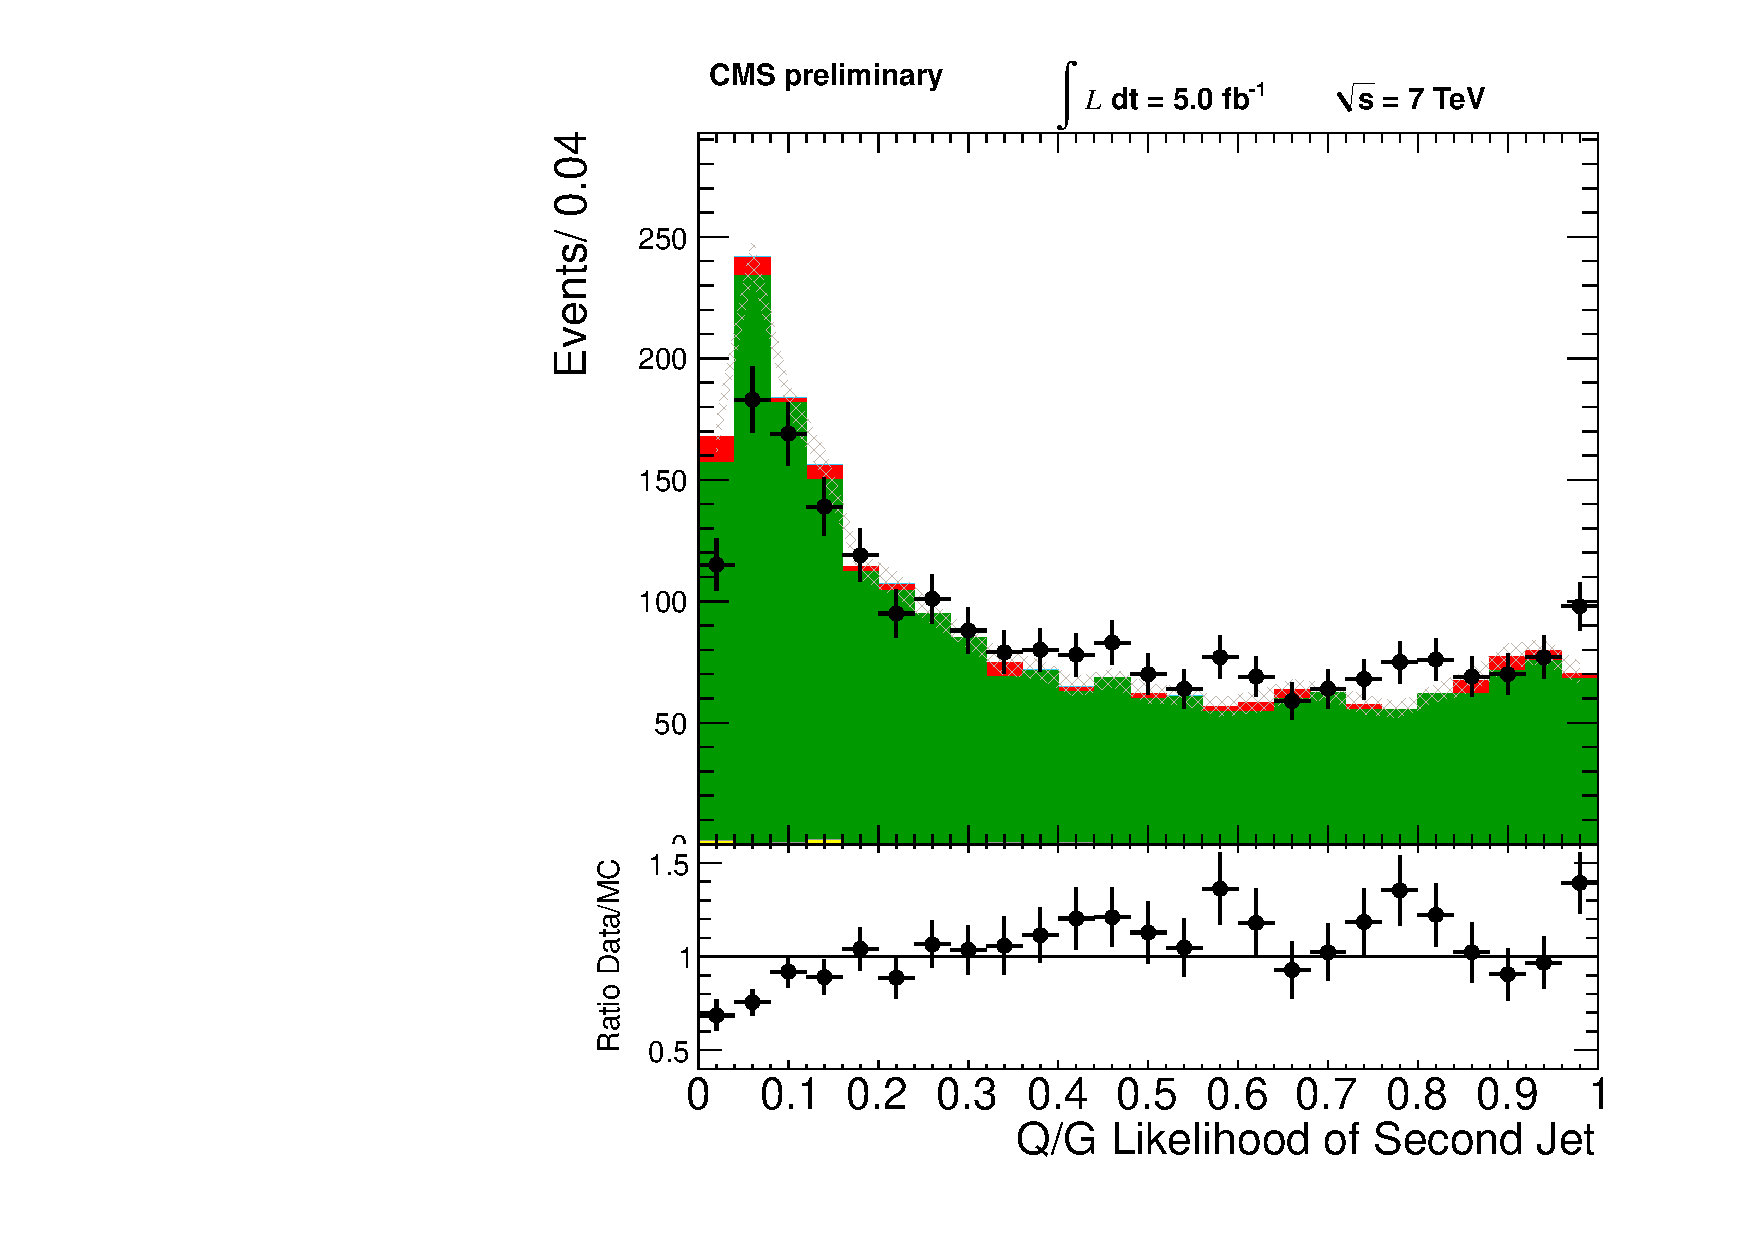
\includegraphics[width=0.49\textwidth]{plots/2012_DataMC/el_jetnt_qgl.pdf}
%%     \caption{Comparison of the Quark-gluon likelihood distributions for leading jet (left)
%%     second leading (right) from data and MC for the electron+jets selection.}
%% \label{fig:elec_jet_qgl}}
%% \end{figure}
% angular variables
%%%%%%%%%%%%%%%%%%%%%%%%%%%%
%%%%%%%%%%%%%%%%%%%%%%%%%%%%
\begin{figure}[h!t]
  {\centering
    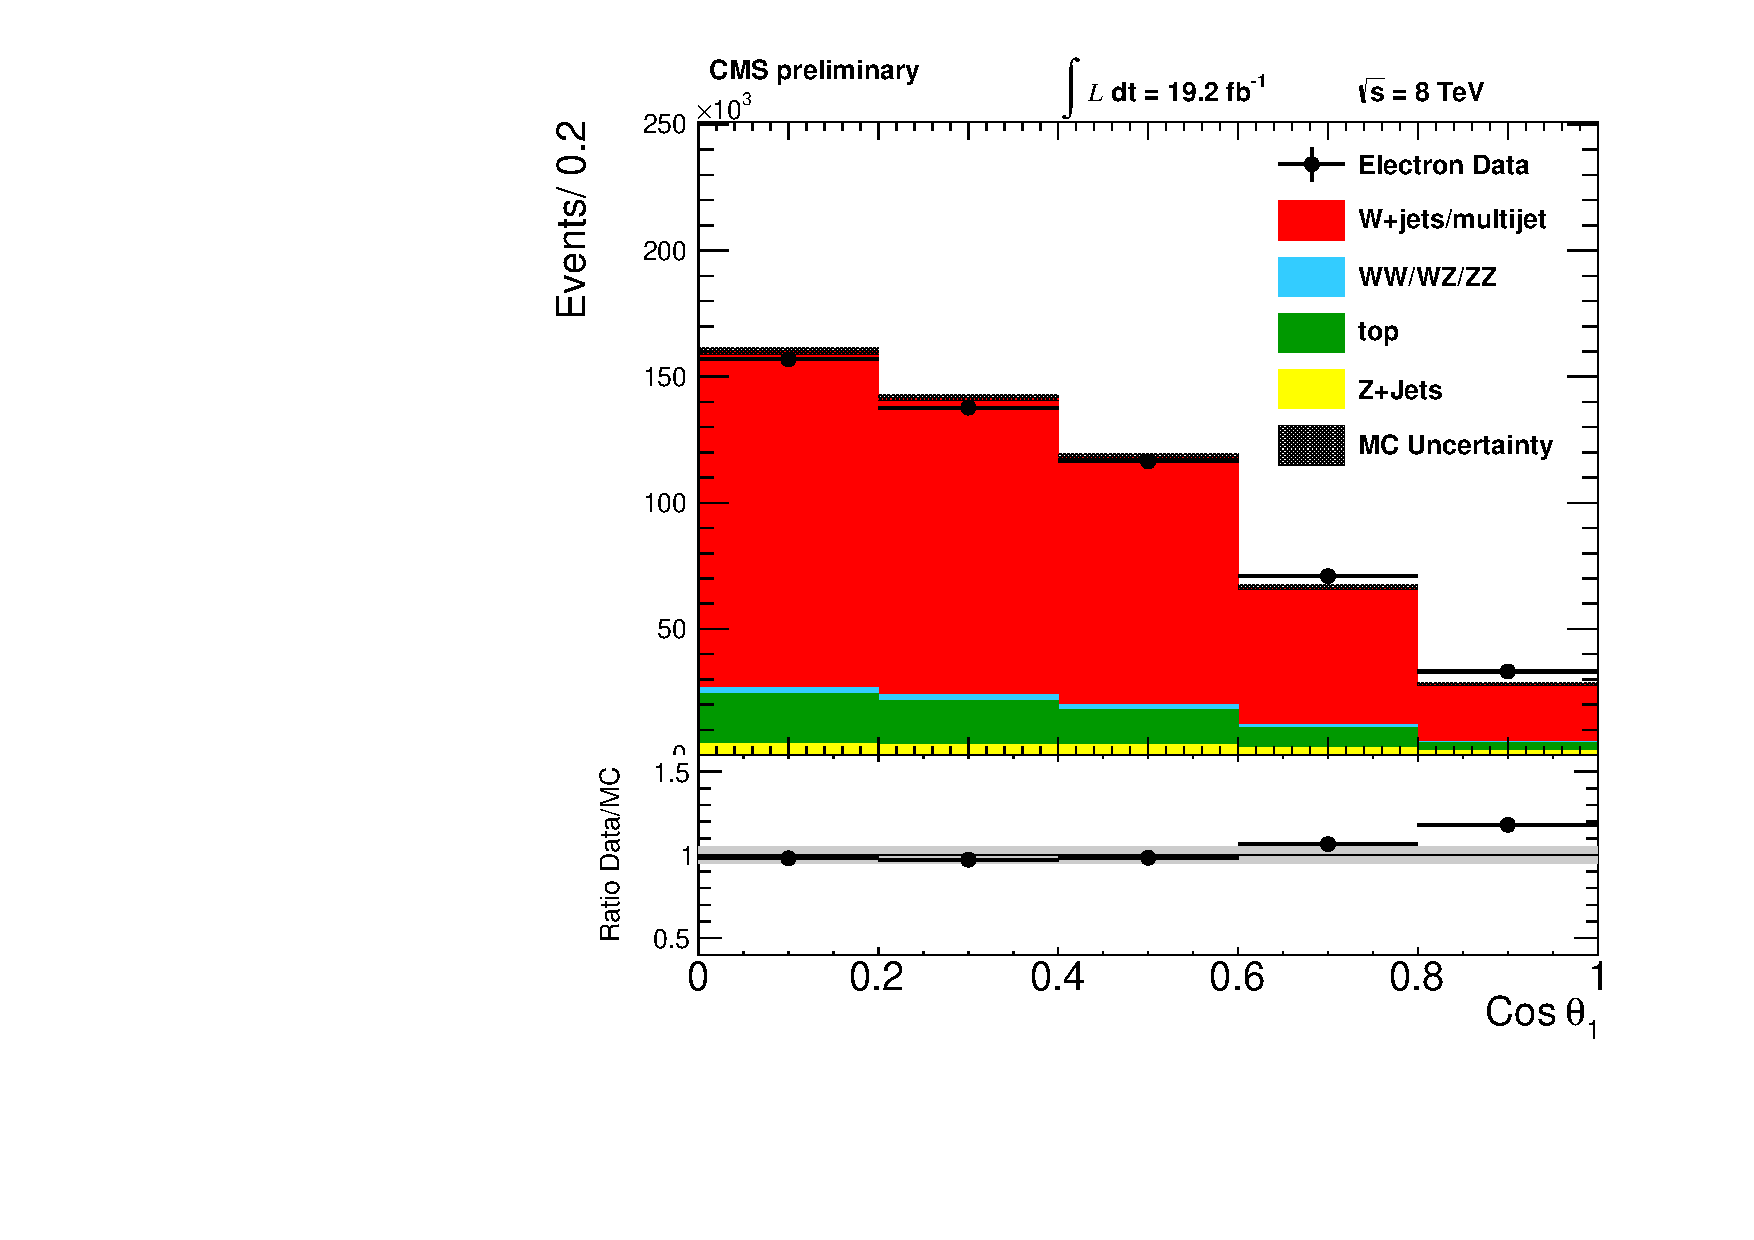
\includegraphics[width=0.49\textwidth]{plots/2012_DataMC/el_ha.pdf}
    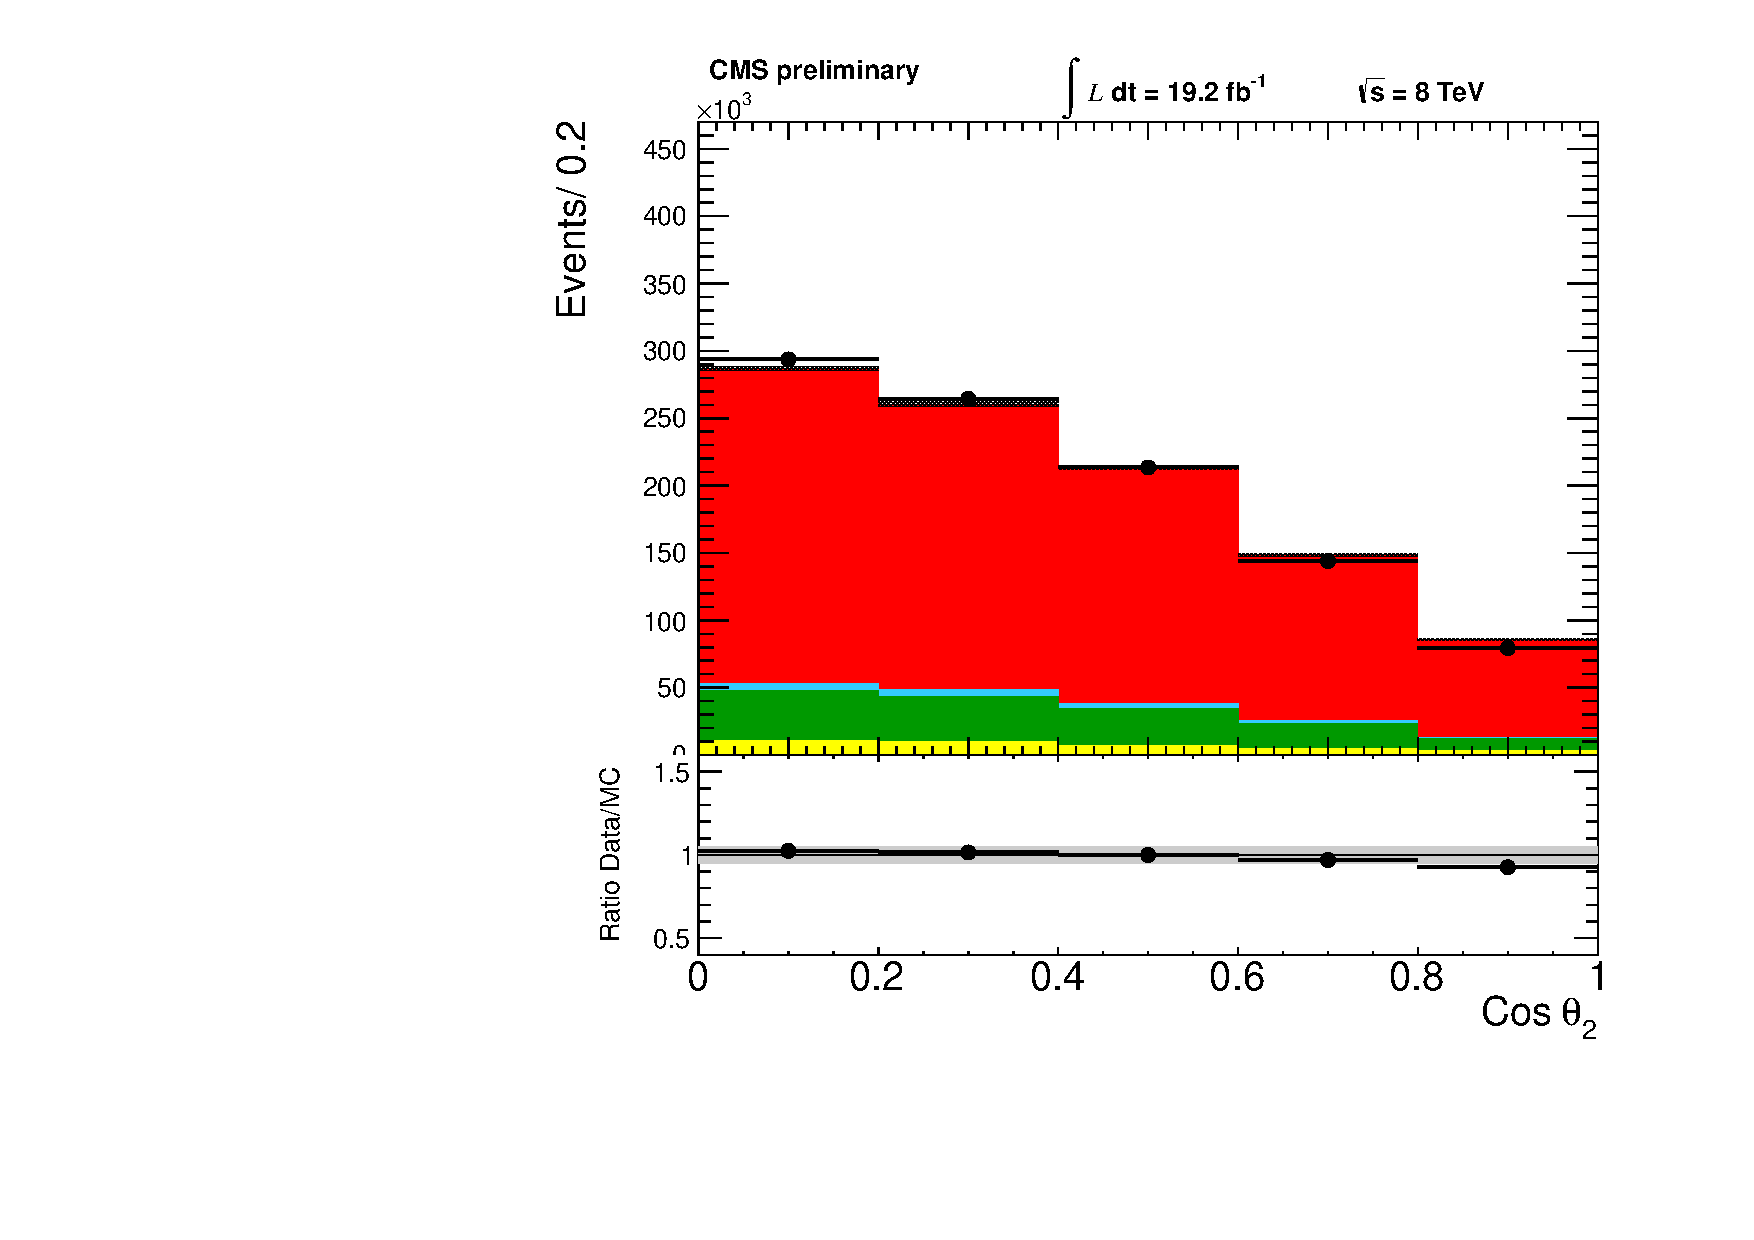
\includegraphics[width=0.49\textwidth]{plots/2012_DataMC/el_hb.pdf}
    \caption{Comparison of the angular distributions for $\cos\theta_{1}$ (left) and
   $\cos\theta_{2}$ (right) from data and MC for the electron+jets selection.}
\label{fig:elec_theta}}
\end{figure}
%%%%%%%%%%%%%%%%%%%%%%%%%%%%
\begin{figure}[h!t]
  {\centering
     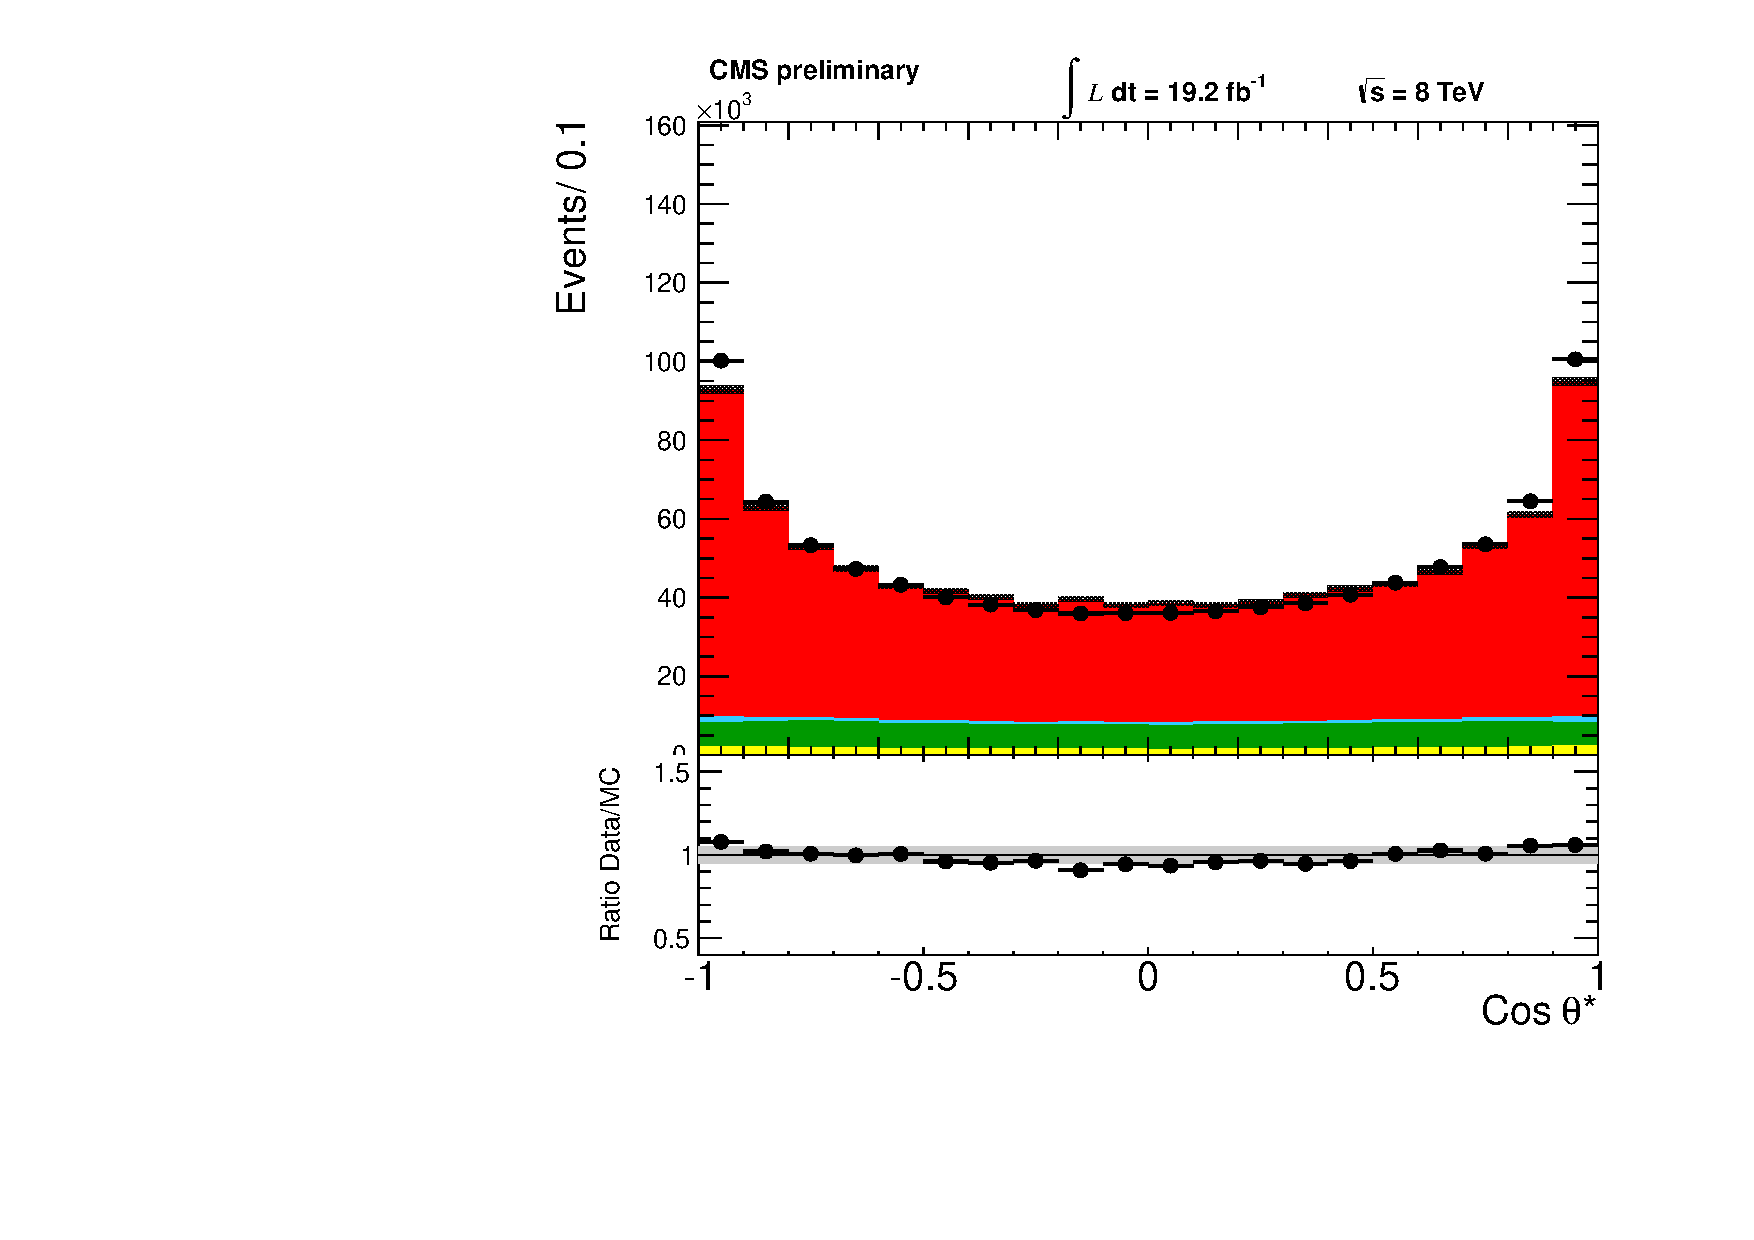
\includegraphics[width=0.49\textwidth]{plots/2012_DataMC/el_hs.pdf}
    \caption{Comparison of the angular distributions for $\cos\theta^{\ast}$ from data and MC 
   for the electron+jets selection.}
\label{fig:elec_thetas}}
\end{figure}
%%%%%%%%%%%%%%%%%%%%%%%%%%%%
\begin{figure}[h!t]
  {\centering
    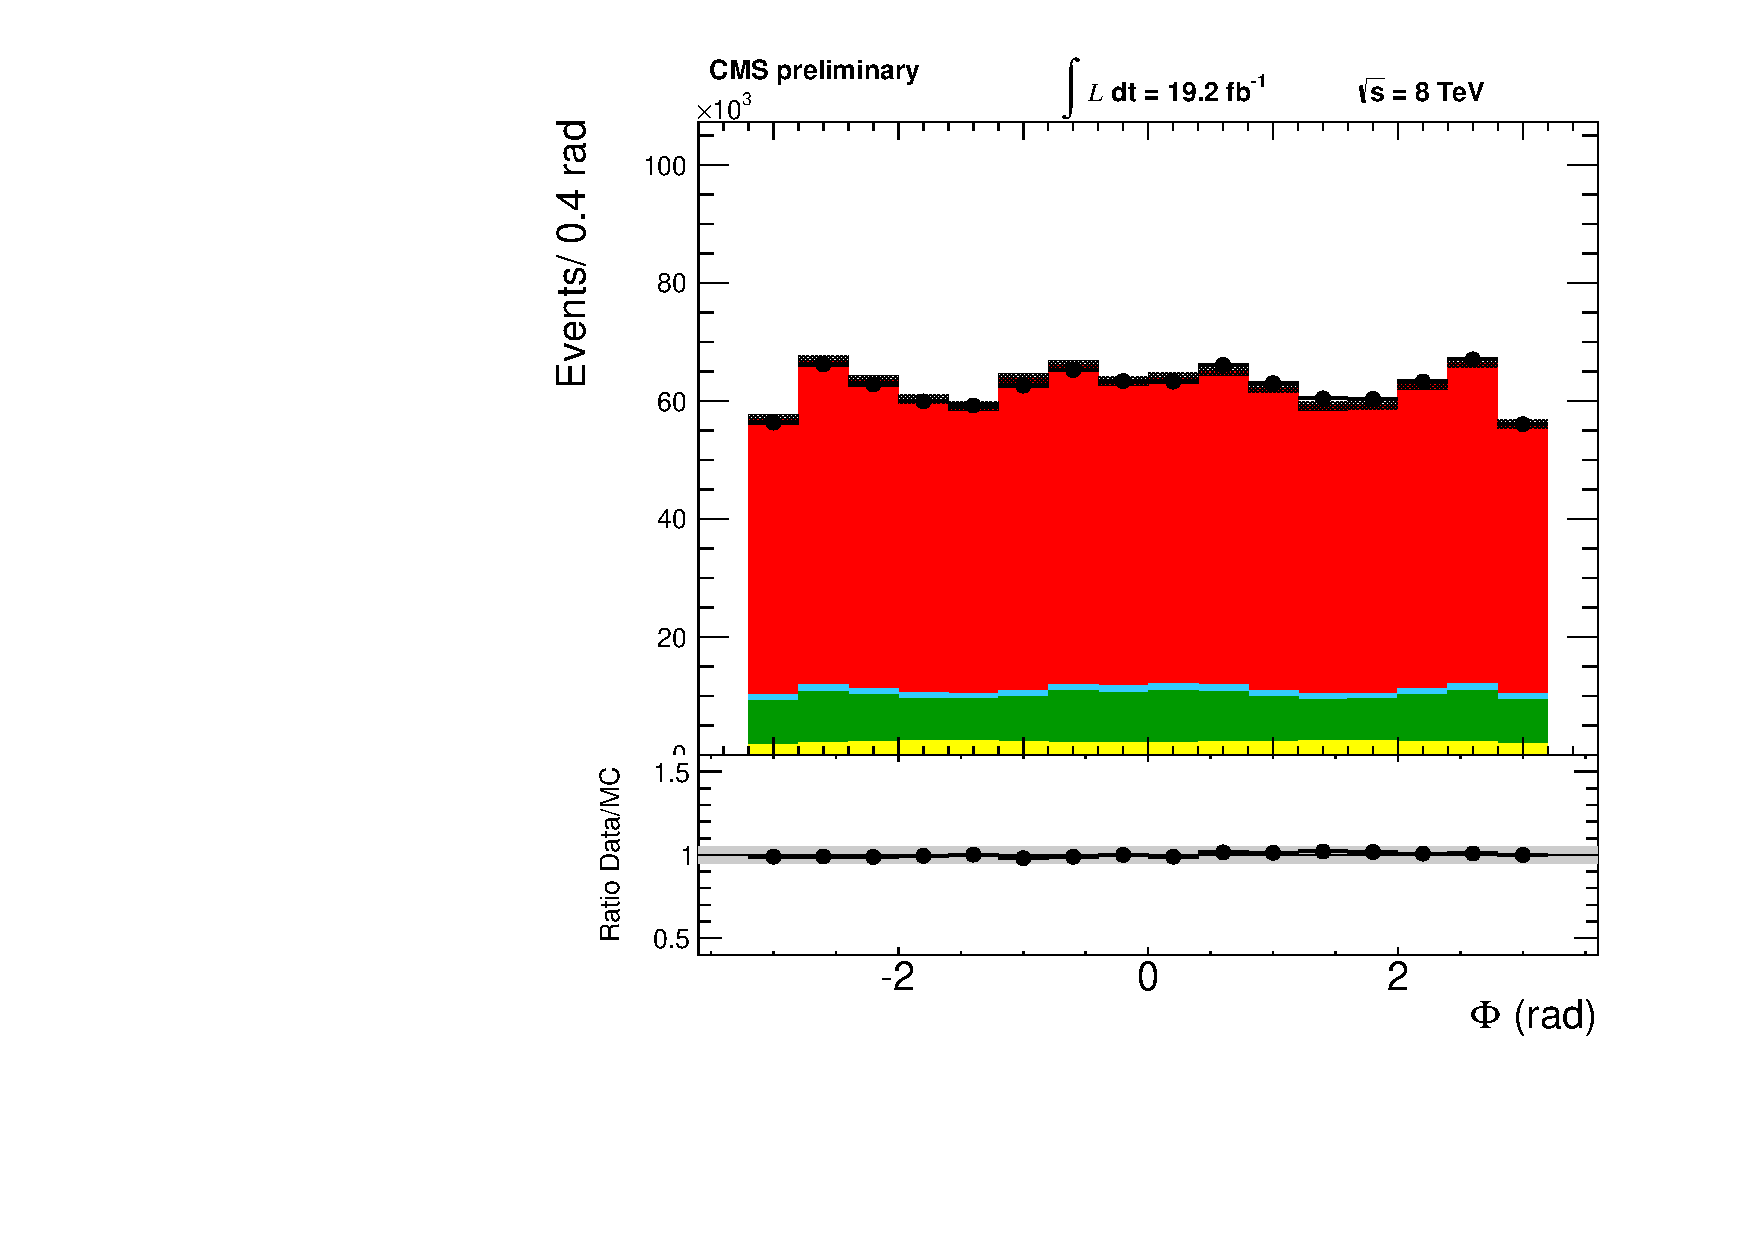
\includegraphics[width=0.49\textwidth]{plots/2012_DataMC/el_phi.pdf}
    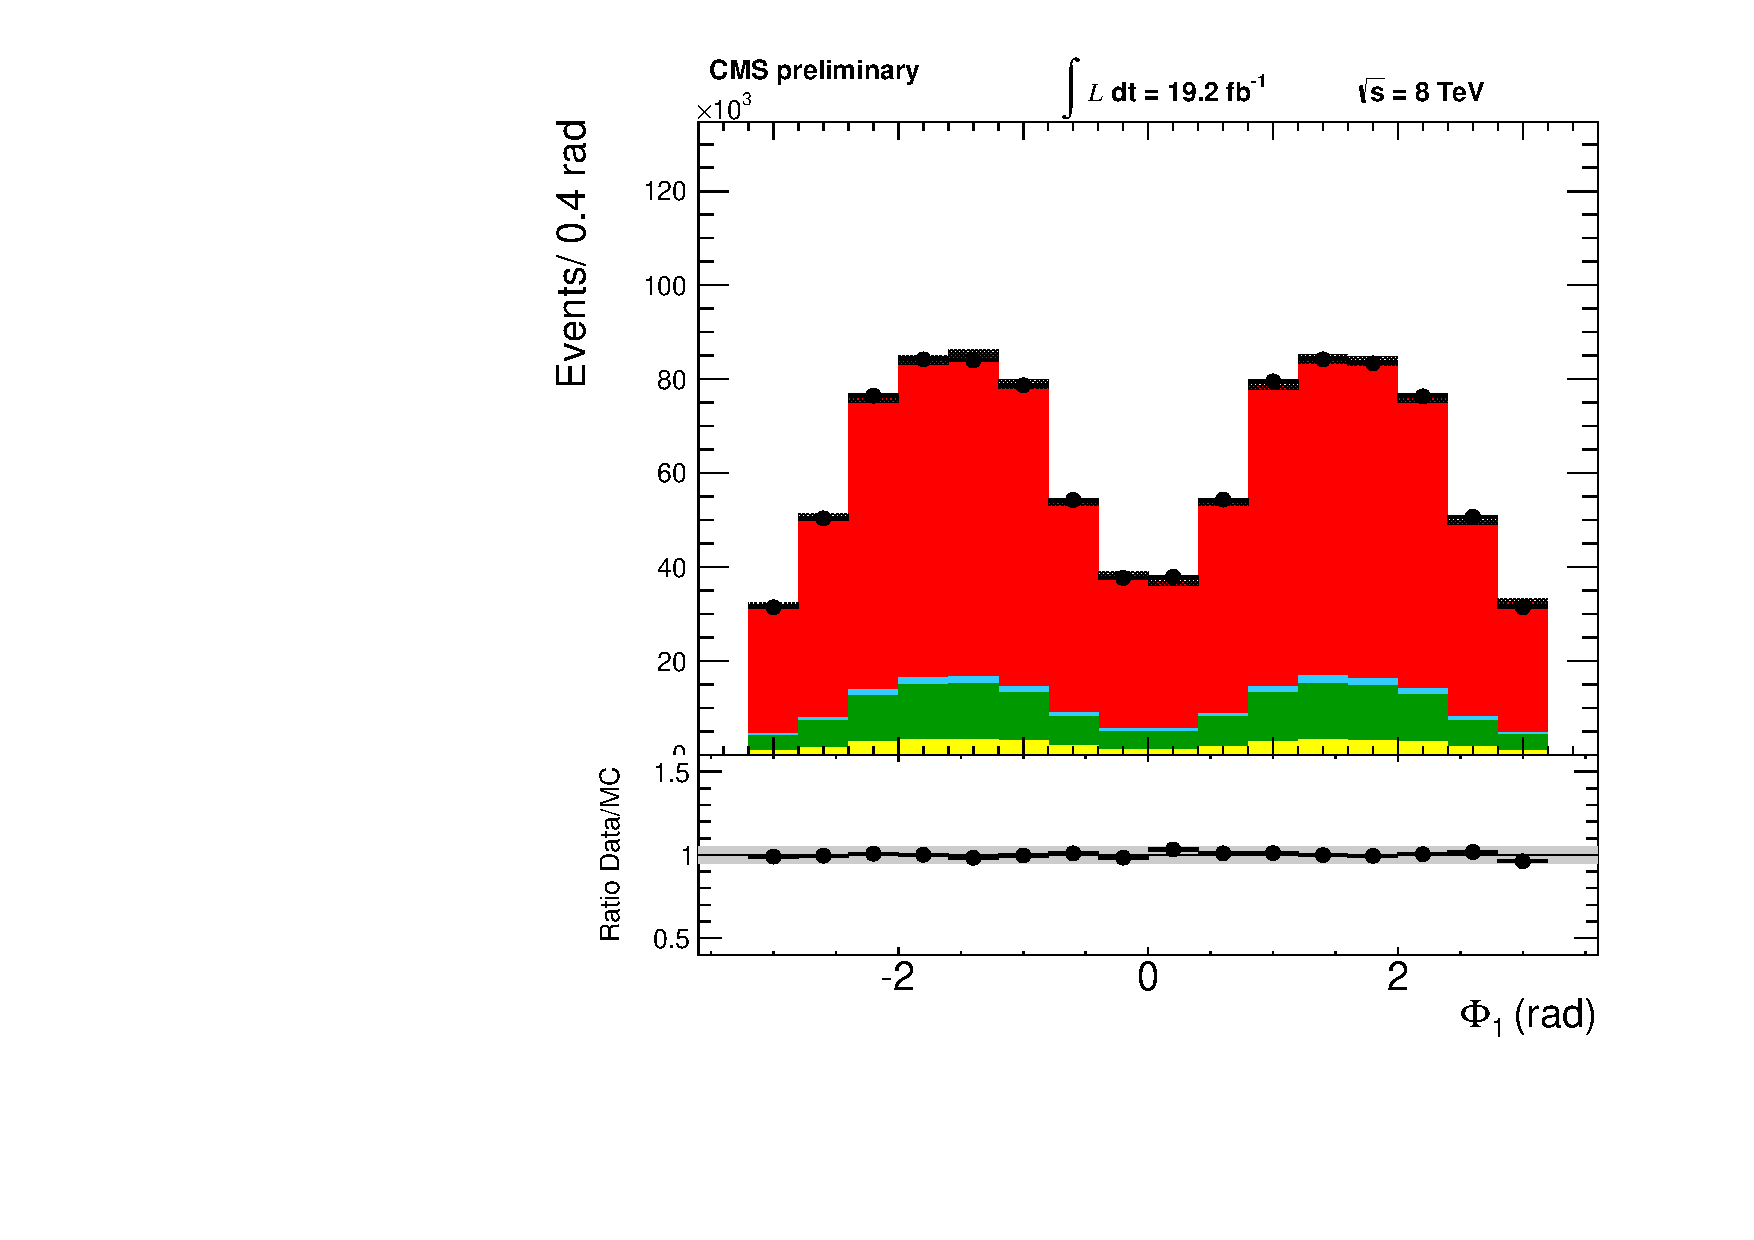
\includegraphics[width=0.49\textwidth]{plots/2012_DataMC/el_phib.pdf}
    \caption{Comparison of the angular distributions for $\Phi$ (left) and
    $\Phi_{1}$ (right) from data and MC for the 
    electron+jets selection.}
\label{fig:elec_phi}}
\end{figure}

%%%%%%%%%%%%%%%%%%%%%%%%%%%%
\begin{figure}[h!t]
  {\centering
    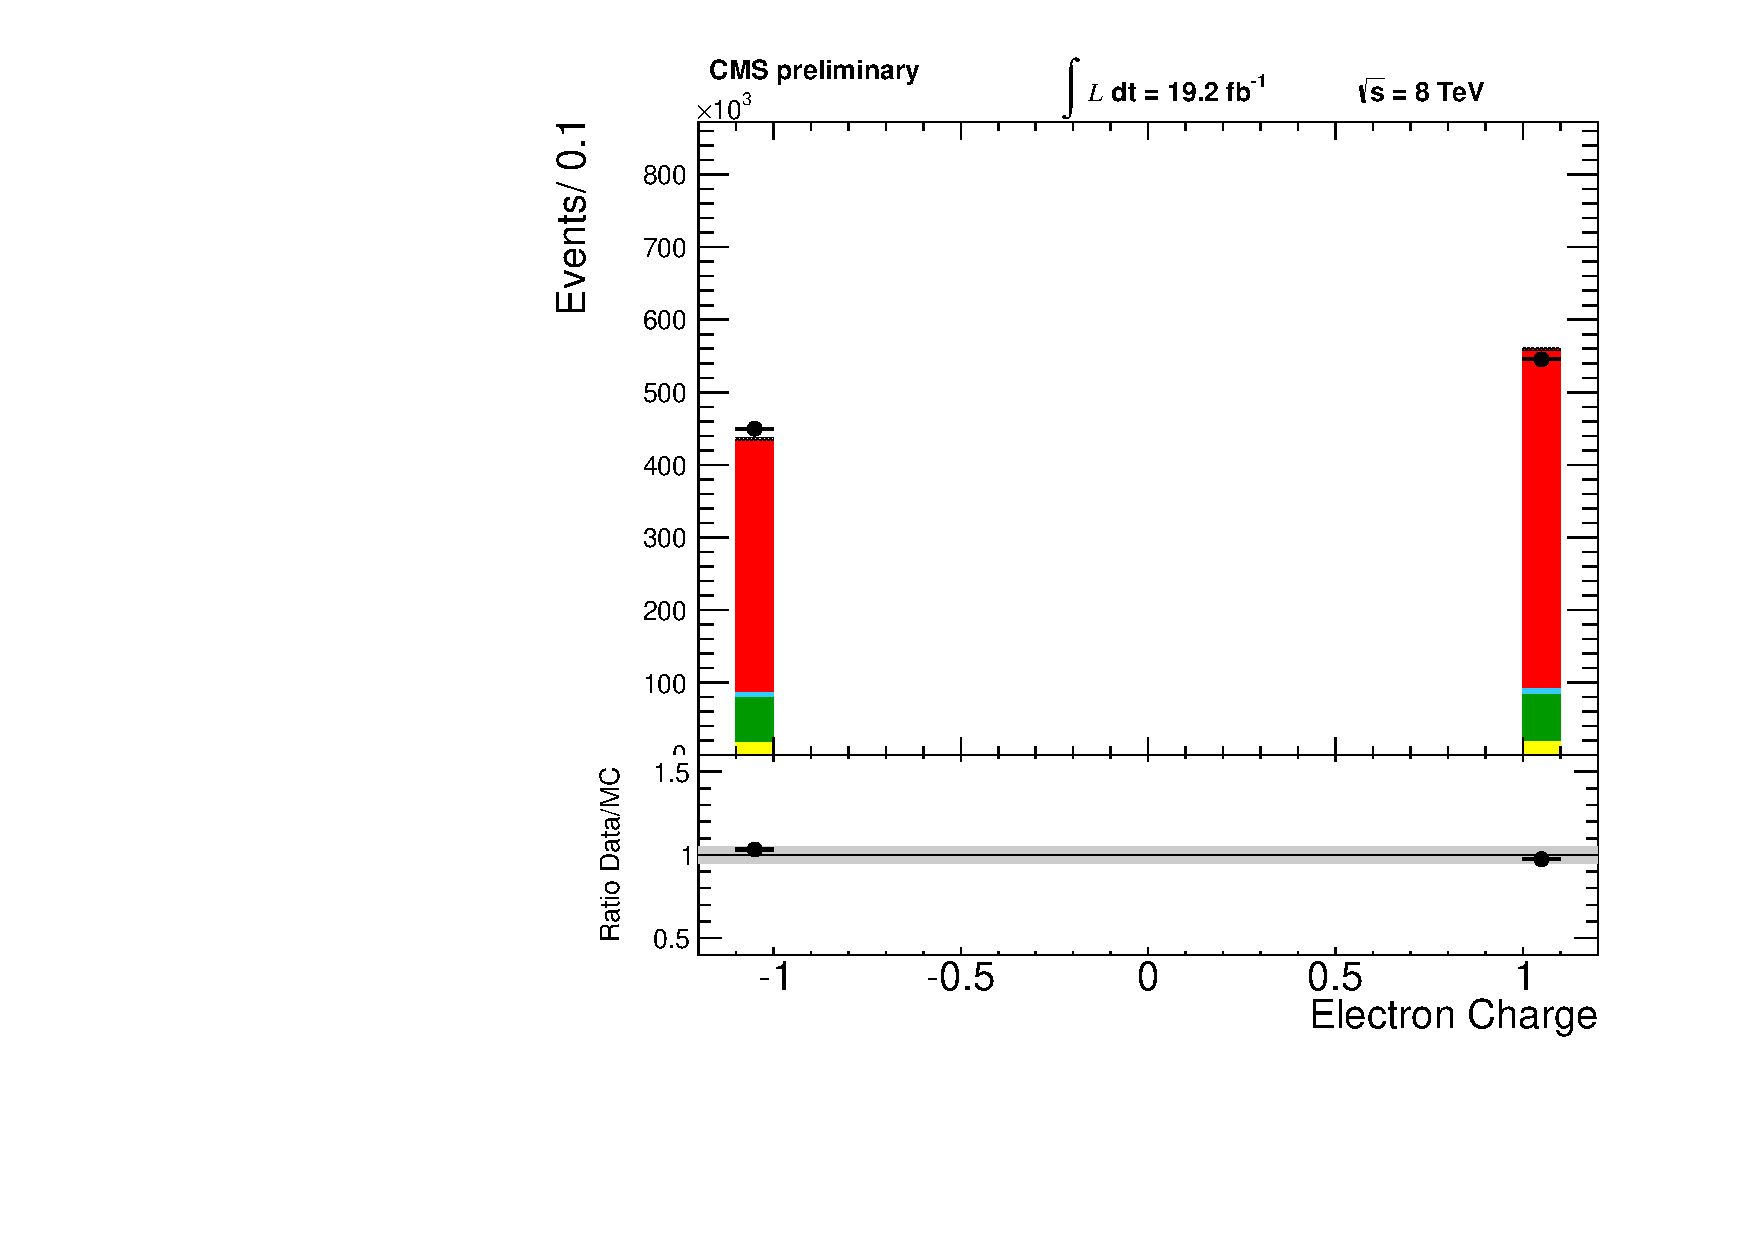
\includegraphics[width=0.49\textwidth]{plots/2012_DataMC/el_charge.pdf}
    \caption{Comparison of the charge of the electron from data and MC for the electron+jets selection.}
\label{fig:elec_chg}}
\end{figure}

% rapidity and pt of the WW system

%%%%%%%%%%%%%%%%%%%%%%%%%%%%
\begin{figure}[h!t]
  {\centering
    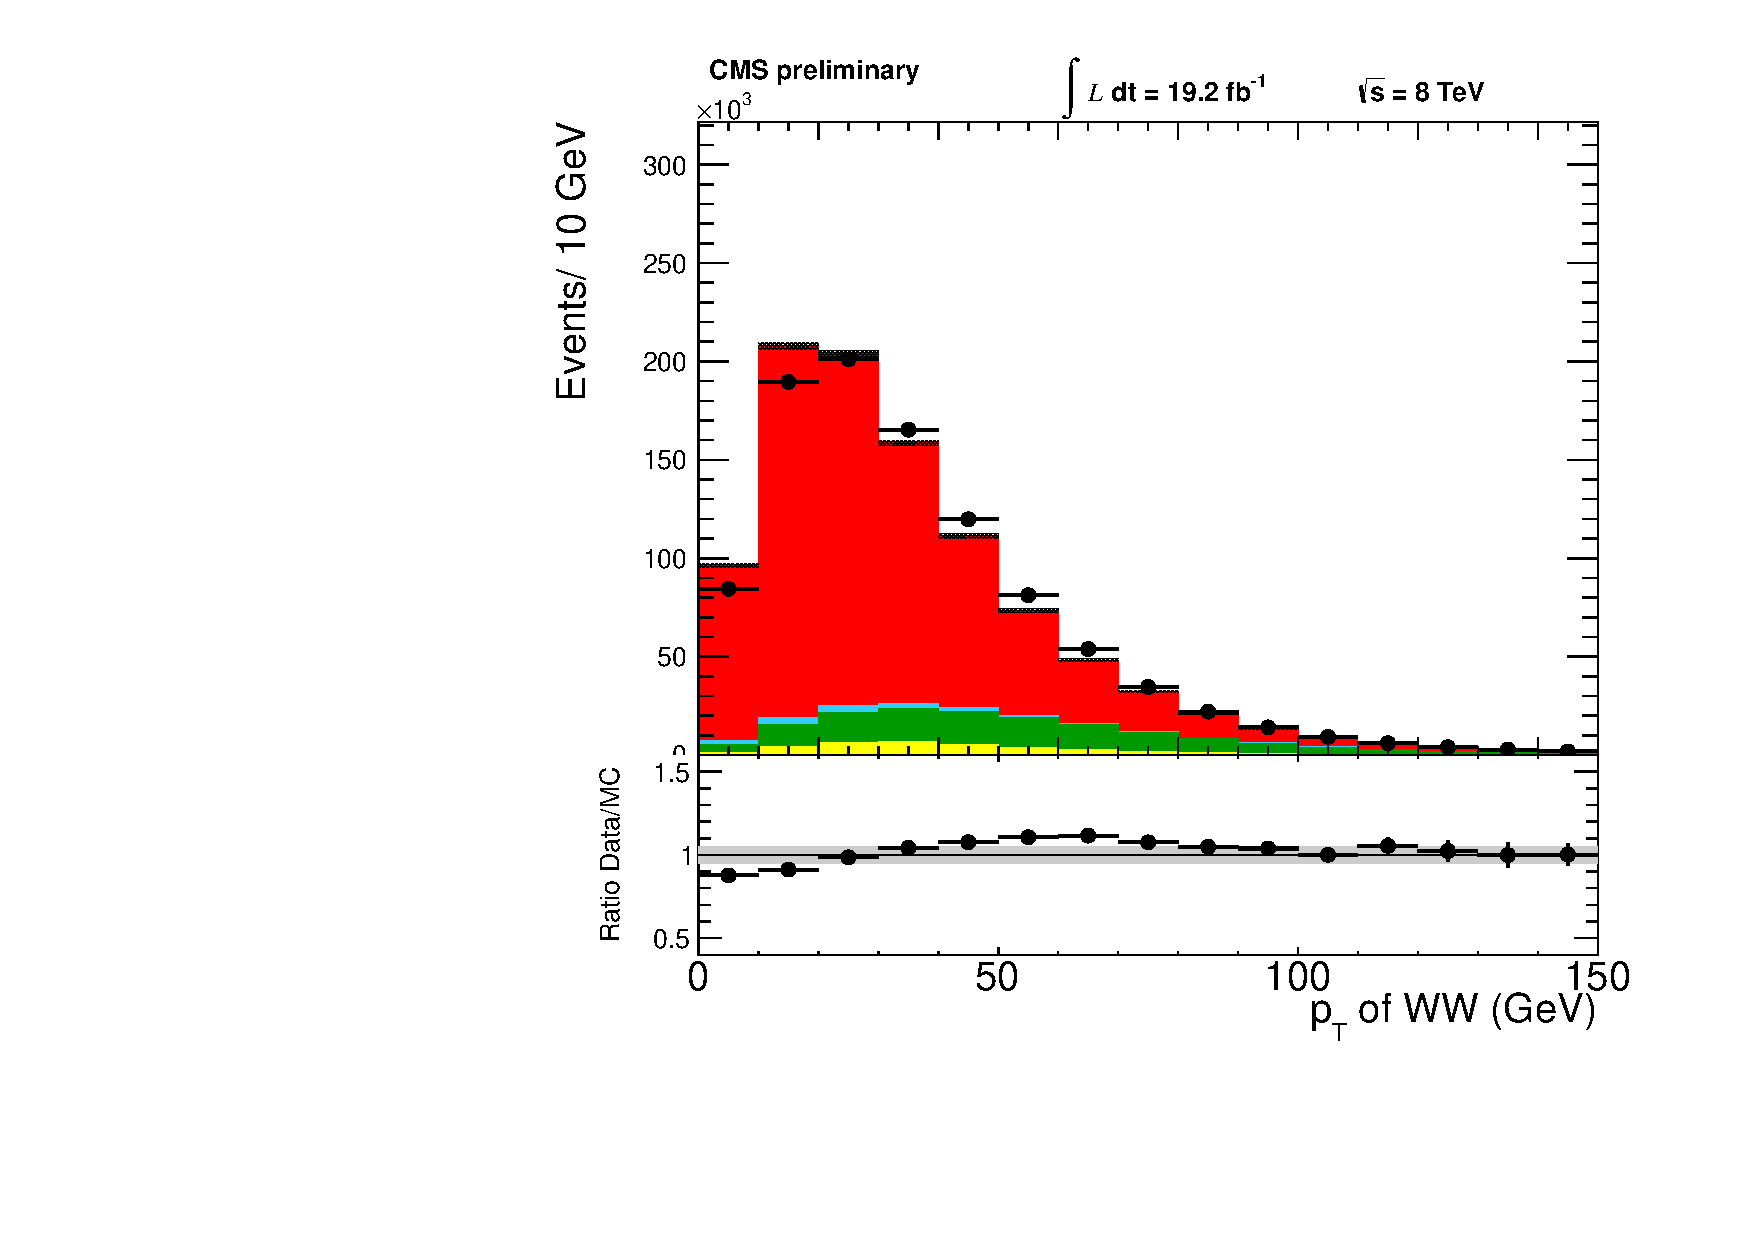
\includegraphics[width=0.49\textwidth]{plots/2012_DataMC/el_ptlvjj.pdf}
    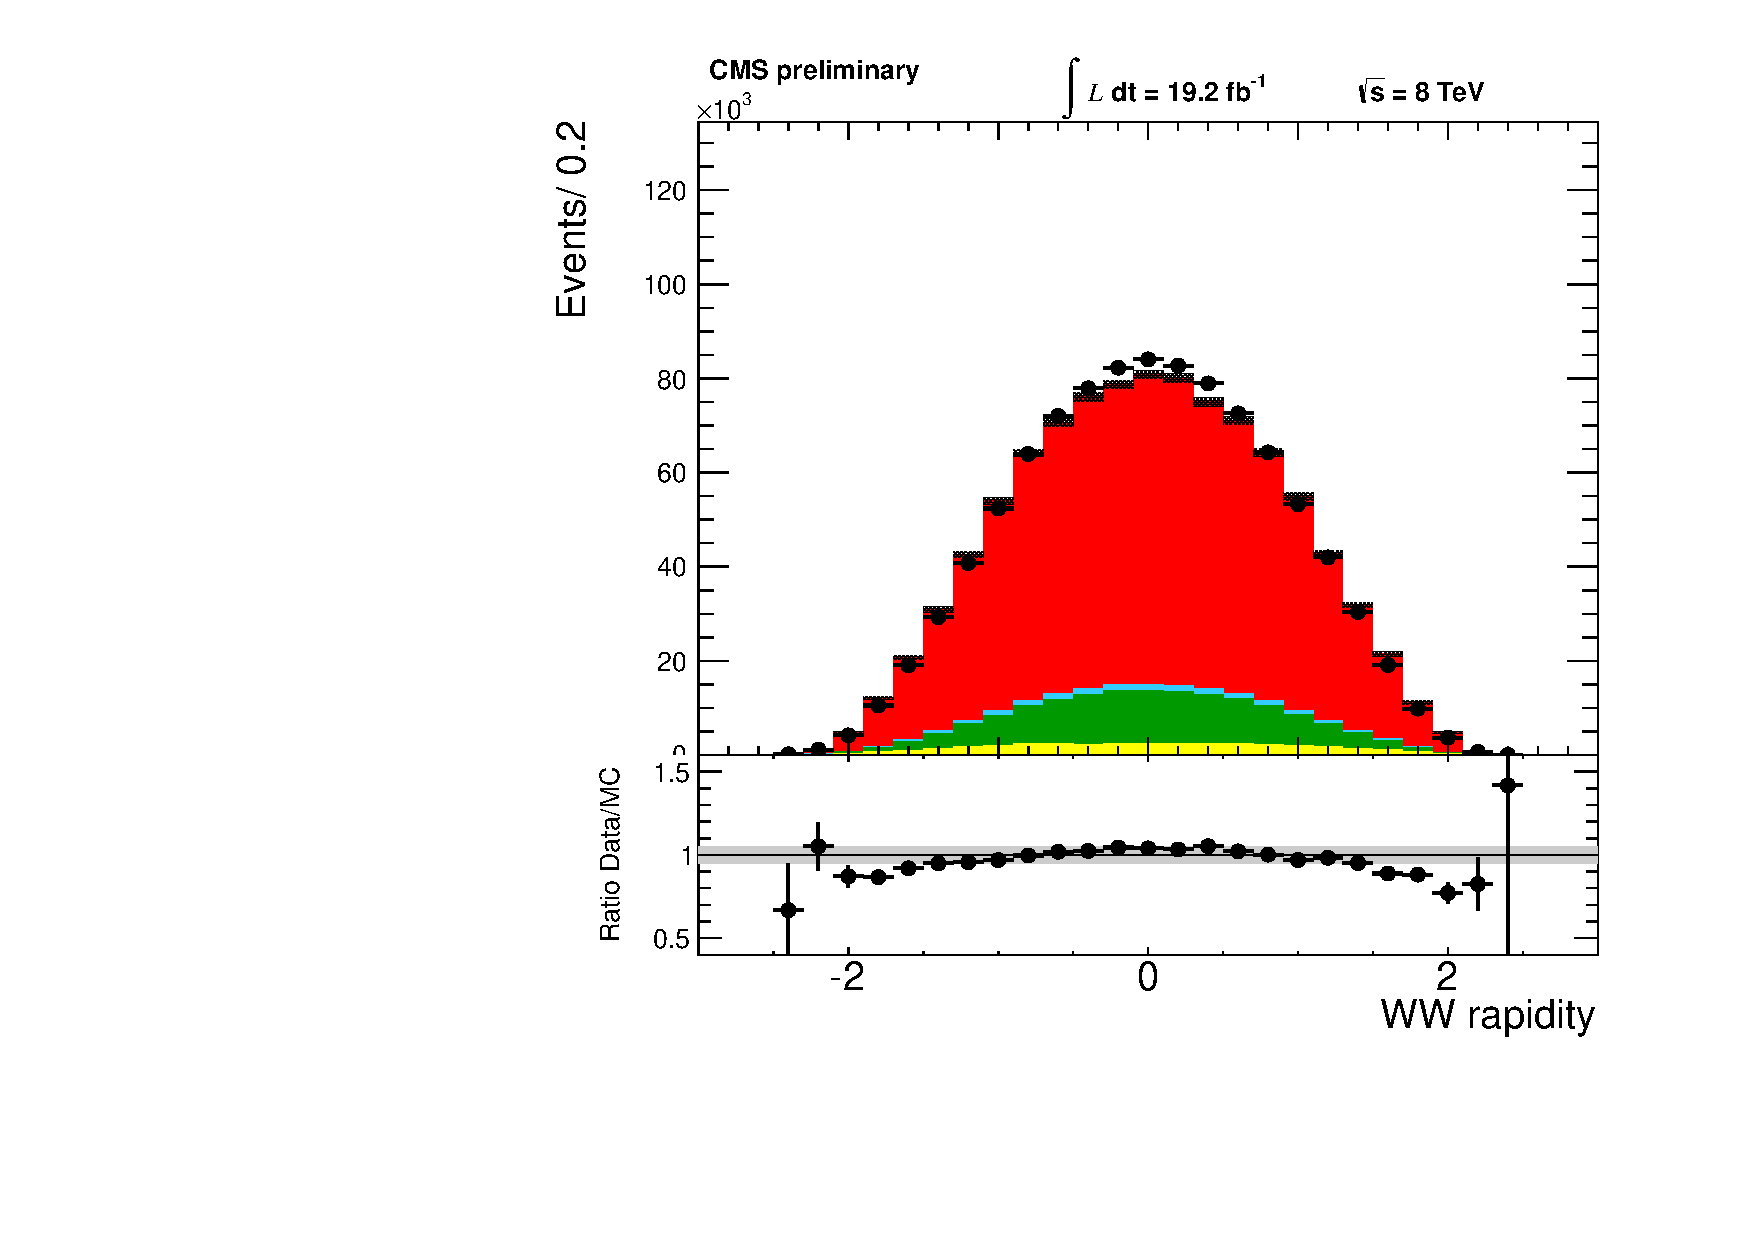
\includegraphics[width=0.49\textwidth]{plots/2012_DataMC/el_etalvjj.pdf}
    \caption{Comparison of the $p_{T}$ (left) and $\eta$ (right) of the WW system
      from data and MC for the electron+jets selection.}
\label{fig:elec_ww}}
\end{figure}

%%%%%%%%%%%%%%%%%%%%%%%%%%%%
\begin{figure}[h!t]
  {\centering
    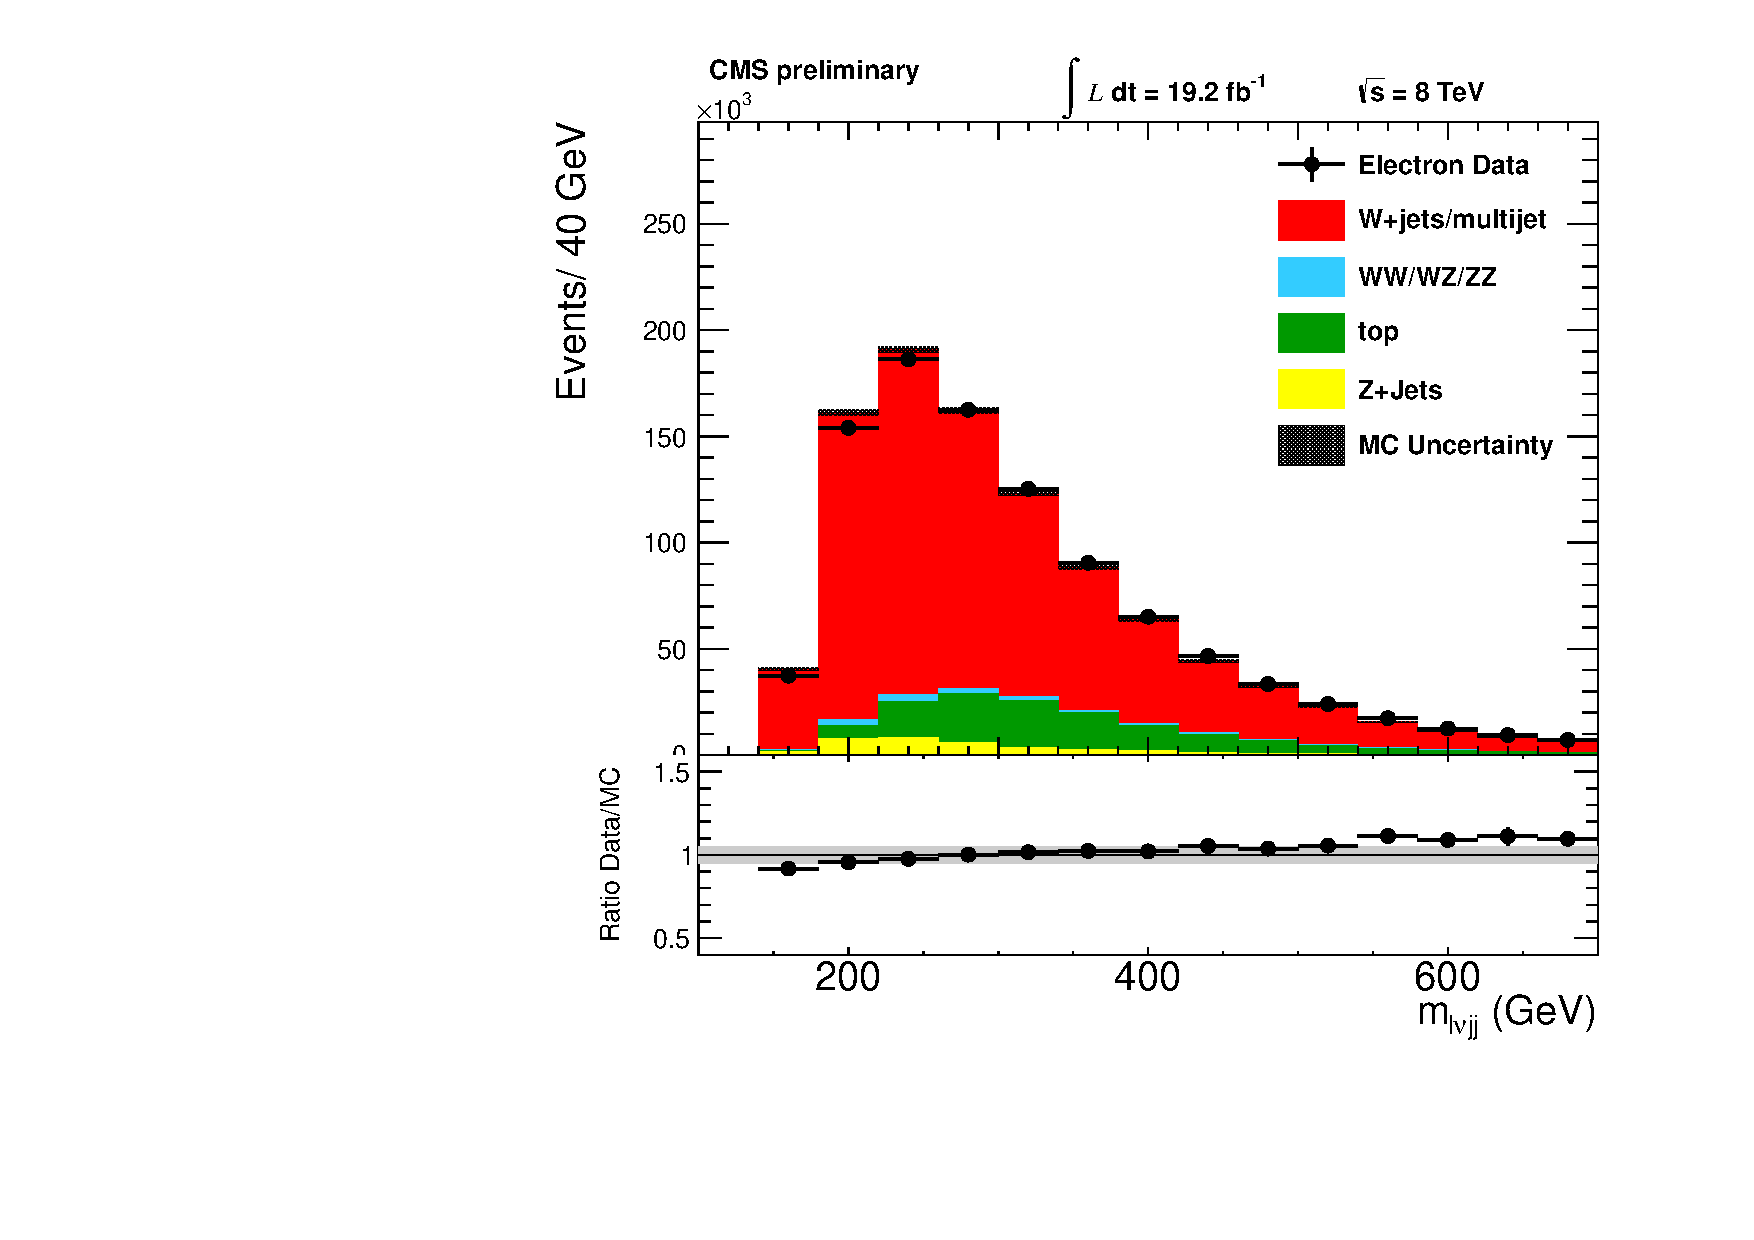
\includegraphics[width=0.49\textwidth]{plots/2012_DataMC/el_mlvjj.pdf}
    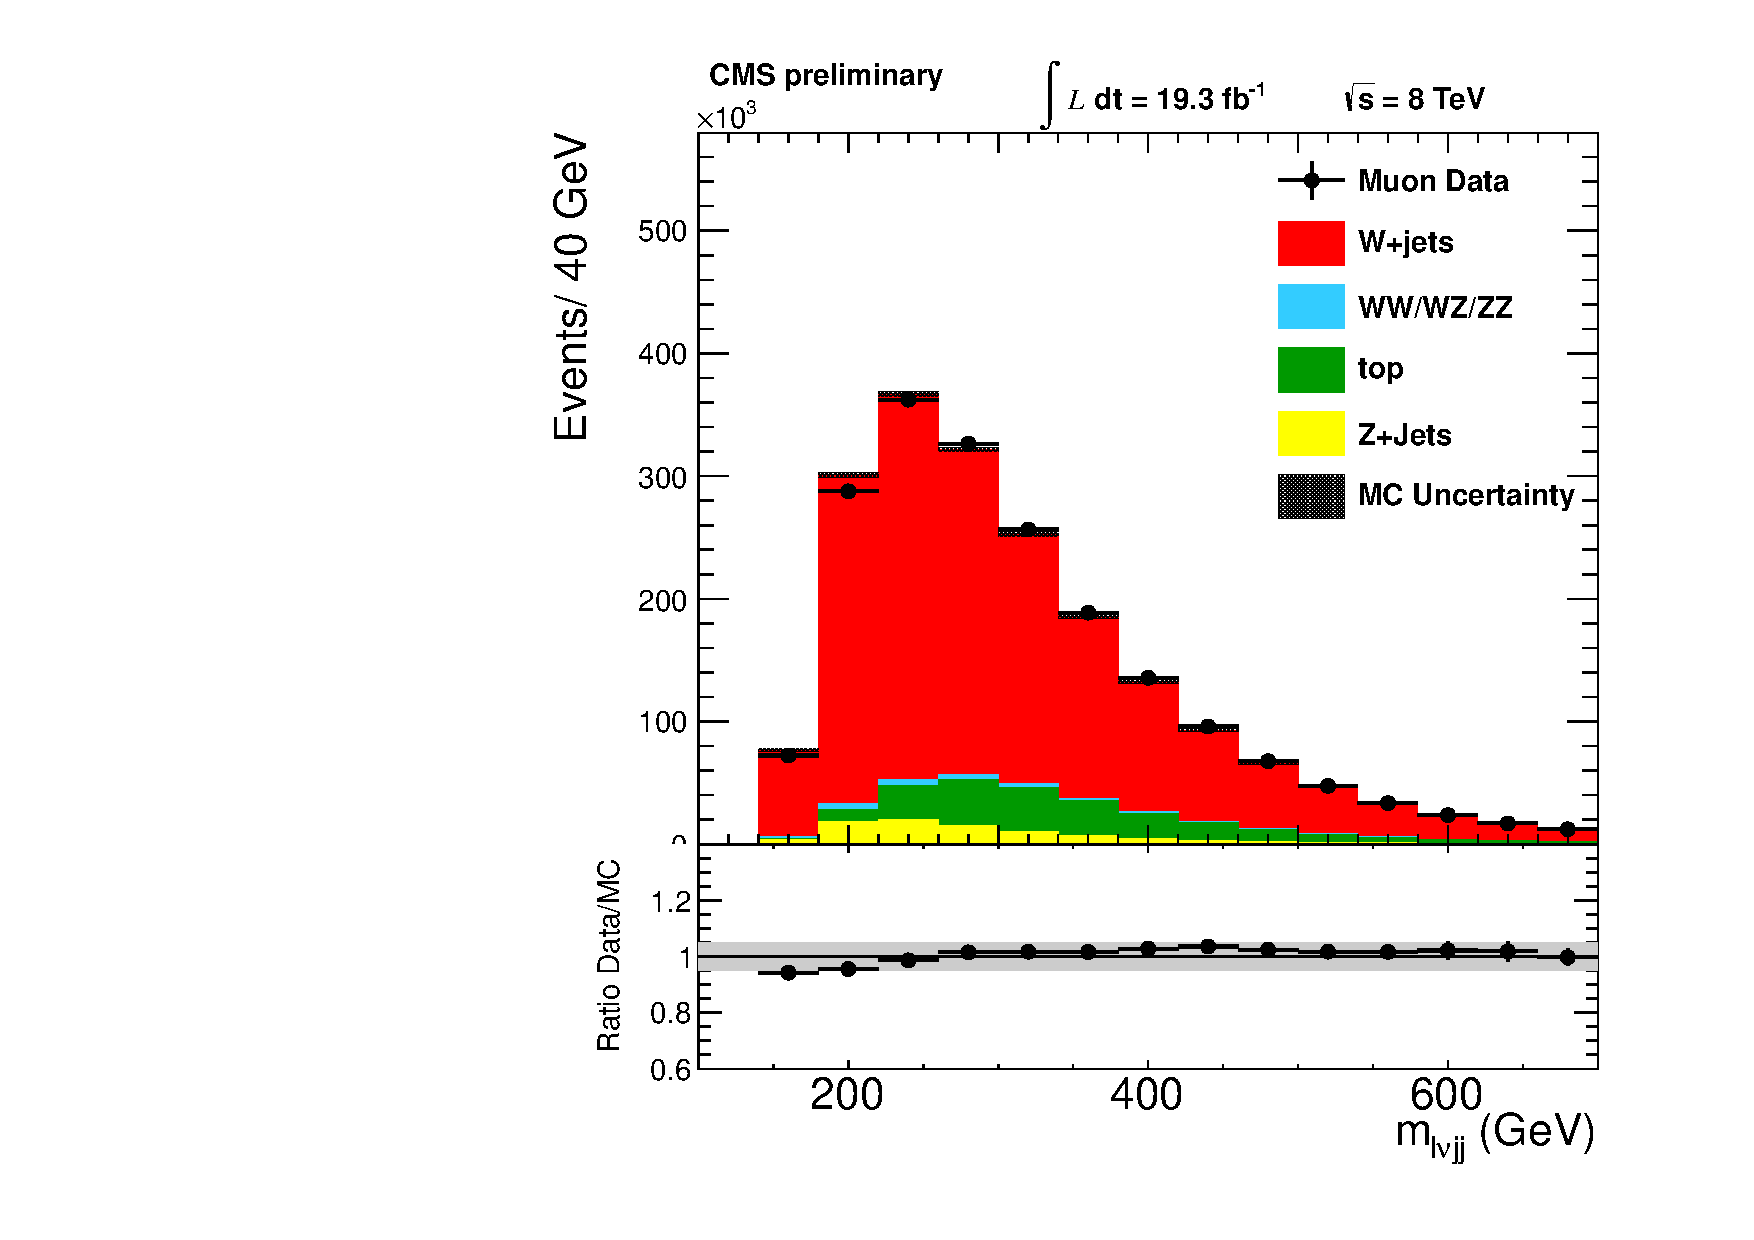
\includegraphics[width=0.49\textwidth]{plots/2012_DataMC/mu_mlvjj.pdf}
    \caption{Comparison of the four-body invariant mass from data and MC for the electron+jets selection (left) 
             and muon+jets selection (right). The disagreement seen here between data and MC for W+jets 
	     background is the motivation for using data-driven shape for W+jets as described in 
	     Section~\ref{sec:wjetsBackground}. }
\label{fig:lep_mlvjj}}
\end{figure}

%%%%%%%%%%%%%%%%%%%%%%%%%%%%%%%%%
%%%%%%%%%%%%%%%%%%%%%%%

